\documentclass[a4paper]{report}
\author{David Gueguen}
\title{Cryptology in smart cards:\\		
		implementations, threats and counter-measures.\\
			Symmetrical \& Asymetrical algs\\						
			}
\usepackage[pdfauthor={David Gueguen},pdftitle={STATeOfTHeARtSmardCardsCryptology},pagebackref,pdftex]{hyperref}	 	
\hypersetup{colorlinks,	
	citecolor=red, filecolor=black, 
		linkcolor=black, urlcolor=blue }
			
%dimension of the sheet
\usepackage[a4paper, no foot,hmargin=1.5cm, vmargin=1.5cm,
			 left=1.4cm, right=1.4cm	]
			 	{geometry}

%packages
\usepackage[latin1]{inputenc}
\usepackage{textcomp}
\usepackage{graphicx}
\usepackage{mathrsfs, amssymb, bbm, amssymb}
\usepackage{amsmath, amsthm, amsfonts, latexsym, stmaryrd}
\usepackage{marvosym}%symbol mail


%algo package old but flexible
\usepackage{epsfig}
\usepackage[linesnumbered,ruled,vlined]{algorithm2e}



\addtocounter{tocdepth}{3}
\setcounter{secnumdepth}{3} 


\setlength{\parskip}{1em}			 	
\setlength\parindent{20pt}		% globally suppress indentation		 	
\medskip						%setup space between pararaph	

%to index
\usepackage{makeidx}
\makeindex	

% Symbols rip, etc -template matrix-
%\usepackage{mathabx}

% allow to use \citeauthor
%\usepackage[numbers,sort]{natbib}
\usepackage{natbib}
%\bibliographystyle{alpha}
%\bibliographystyle{apalike} moche
\bibliographystyle{plainnat}
%\bibliographystyle{abstract}	
%\bibliographystyle{plainnat}%isbn et doi
% allow to use \citeauthor
%\usepackage[numbers,sort]{natbib}



% Tables
\usepackage{colortbl}
\usepackage{tabularx}
\usepackage{supertabular}
\usepackage{multirow}
\usepackage{relsize}
\usepackage{longtable}

%theorme package
\usepackage{amsthm}
\usepackage{mathrsfs}
% Landscape pages
\usepackage{pdflscape}
\usepackage{pdfpages}

%Footnote for array (to place after the colour package)
\usepackage{footnote}
\usepackage{natbib}
%\usepackage[sort&compress]{natbib}

%%%%%%%%%%%%%%%%%%%%%%%%%%%%%%%%%%%%%%%%%%%%%%%%%%%%%%%%%%%%%%%%%%%%%%%%%%%%%%%%%%%%%%%%%%%%%%%%



\newcommand{\bld}[1]{
	\mbox{\boldmath $#1$}
		}

\renewcommand{\thechapter}{
	\Roman{chapter}
		}

\newcommand{\bigO}[1]{
 	\ensuremath{\mathop{}\mathopen{}\mathcal{O}\mathopen{}\left(#1\right)}
 		}	
%\newcommand{\smallO}[1]{
%	\ensuremath{\mathop{}
%		\mathopen{{\scriptstyle\mathcal{O}}\mathopen{}\left(#1\right)}}



% asterisc allow unumbered theorem
\newcommand{\defi}[1]{  \textbf{Definition : #1 }}

	%% add this
	\let\oldUrl\url\renewcommand{\url}[1]{\href{#1}{$\mathscr{L}$ink}}
	
	\newcommand{\urlloki}[1]{ 
		\href{https://choucroutage.com/Papers/SideChannelAttacks/#1} 
			 {\raggedleft \color{blue}$\mathscr{L}ink$\color{black} \raggedright }     }
	
	\newcommand{\lokiquote}[1]{
		\cite{#1}, \urlloki{#1.pdf}
		}
	

\theoremstyle{definition}
\newtheorem*{mydef}{Definition}
\theoremstyle{plain}
\newtheorem*{mythm}{Theorem}
\theoremstyle{plain}
\newtheorem*{myprop}{Proposition}
\theoremstyle{plain}
%%\newtheorem{lem}[thm]{Lemma}
	
%%%%%%%%%%%%%%%%%%%%%%%%%%%%%%%%%%%%%%%%%%%%%%%%%%%%%%%%%%%%%%%%%%%%%%%%%%%%%%%%%%%%%%%%%%%%%%%%			
\begin{document}
	\maketitle			
	    	\begin{center}
		\Huge{\textbf{WARNING: .....Work in progress!}}
	\end{center}
\large
\label{Objective}
	
\subsection*{Principles}
This is an interactive document: It shall be modified on demand. \\
Each time, for each suggestion: mistakes, typos, a missing topics, something not clear, etc... 
\begin{center}
	E-mail \Letter: 
	\urlstyle{rm}
	\href{mailto:davidgueguen2000@yahoo.fr}{davidgueguen@mdl29.net}				
\end{center}
\begin{itemize}
	\item If you don't understand something this document is crap!	
	\item \lokiquote{sigmobile-2011-shannon}: link to pdf via choucroutage.com 
	\item \href{http://en.wikipedia.org}{Link}: link to wikipedia 
\end{itemize}

\subsection*{Objective}

\begin{itemize}	
\item The only reason for this document is to help in the understanding of an
	 attack/implementation. Tell if useful or not, pleaze, if there are thing missing.
	 
\item This document is far away from being enough to understand many modern attacks,
	for this reason it is mainly focus on implementation.	
\end{itemize}
As feasible as it is possible, was tried to make this document as precise and exact as possible 
on a mathematical point of view introducing systematically some required mathematical vocabulary. \\

To do :\\
*  give -anonymous- benchmark\\
*  give a precise estimation of the complexity, numerical examples\\
*  make system of references reliable  \\
*  refine the indexes of frequency\\
*  provide practical and theoretical ($\pm$) traces 

\subsection*{Thanx}
			\begin{figure}[h]
			\begin{center}
				
\includegraphics[scale=0.66]{images/logorfi.jpg}\\			\vspace{3mm}
	       		
\includegraphics[scale=4]{images/logoul.png}\\				\vspace{3mm}
	       		
\includegraphics[scale=0.66]{images/logoapplus.png}\\ 		\vspace{3mm}
	       		
\includegraphics[scale=0.75]{images/logochoucroutage.jpg}\\
			\end{center}
			\end{figure}


	\newpage
		\begin{figure}[h]
		\begin{center}
	       		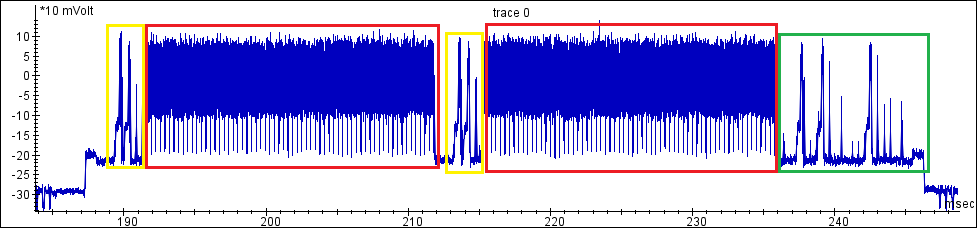
\includegraphics[width=18cm,height=5.5cm]{images/fullrsa.png}\\			\vspace{5mm}
	       		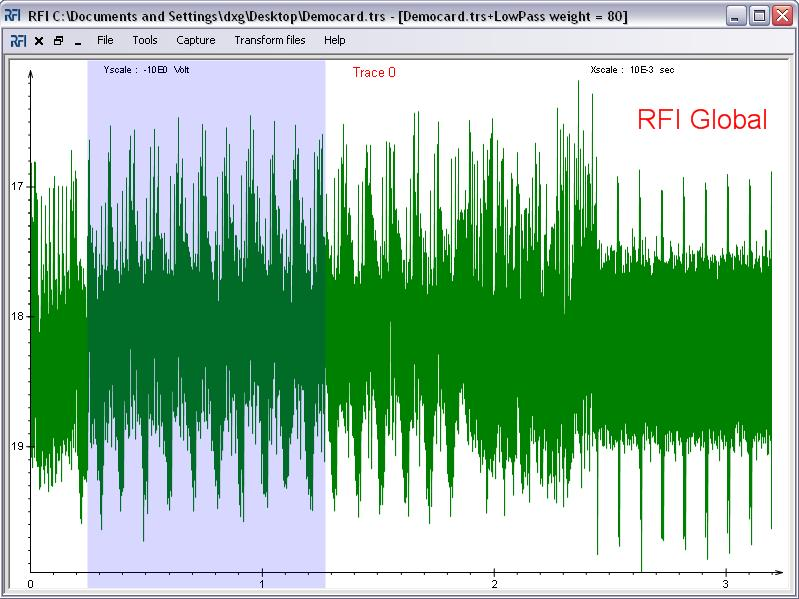
\includegraphics[width=18cm,height=5.5cm]{images/1.JPG}\\				\vspace{5mm}
	       		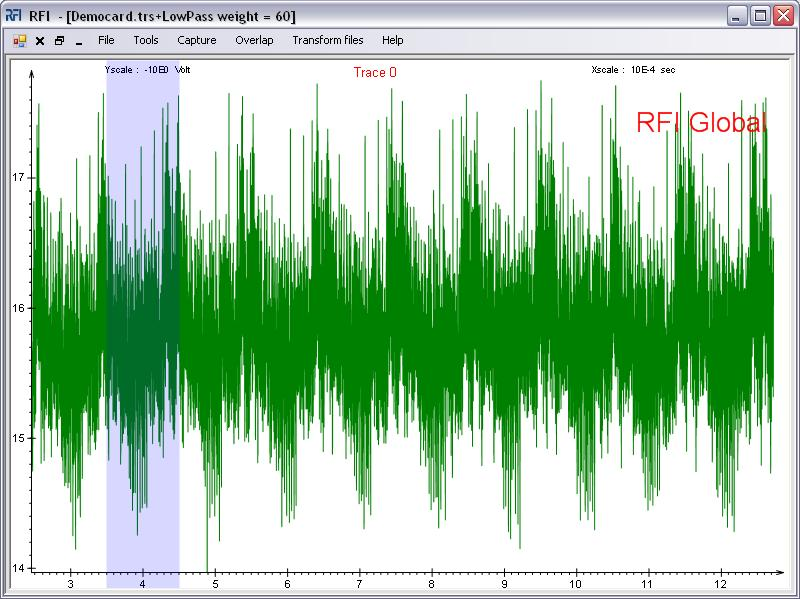
\includegraphics[width=18cm,height=5.5cm]{images/2.JPG}\\				\vspace{5mm}
	       		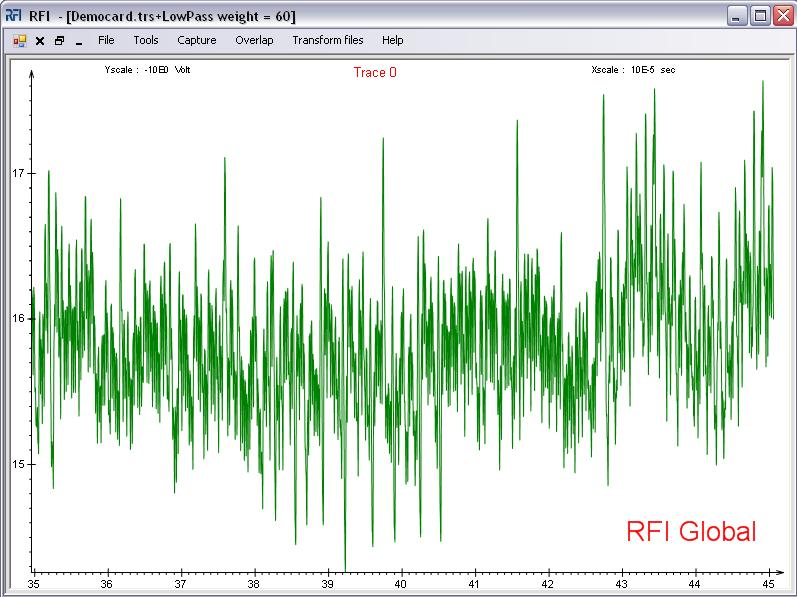
\includegraphics[width=18cm,height=5.5cm]{images/3.JPG}\\	
		\end{center}
		\end{figure}
	\newpage
	\tableofcontents

	    	\chapter{Symmetric encryption}	
	    		\section{Intro}
\label{SymmetricalIntro}

Symmetrical cryptography relies on Claude Shannon's 'theory of Information':
quantify amount of information inside a theoretical channel.
\begin{center}		
	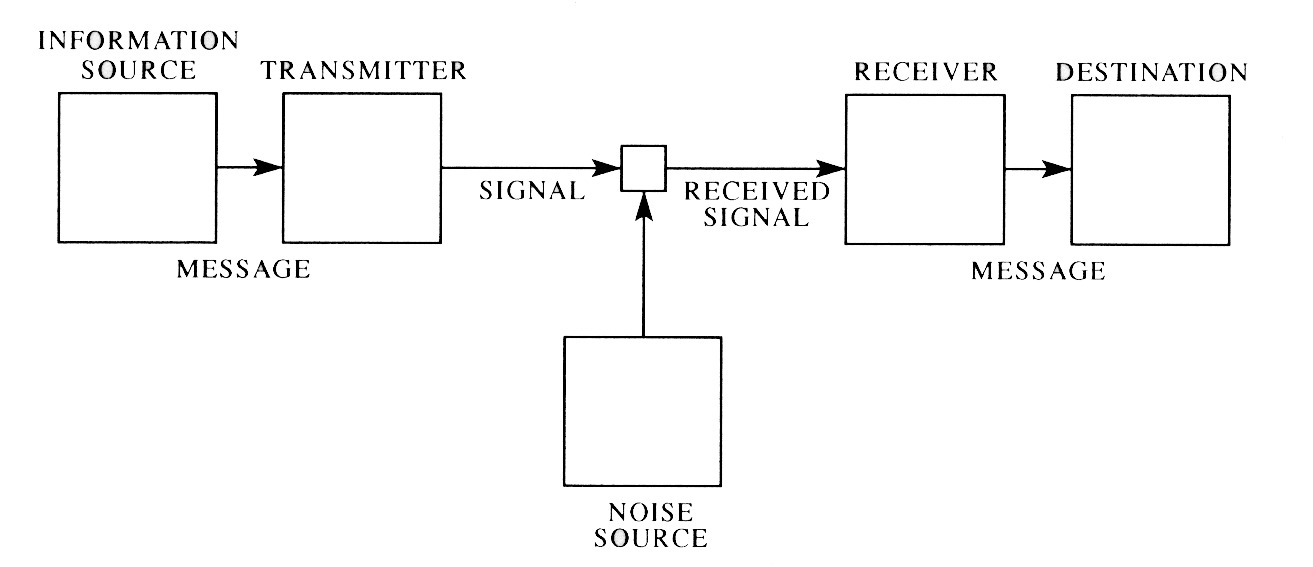
\includegraphics[width=18cm,height=5cm]{images/shannon.jpg}
\end{center}
Classical concepts: entropy, noisy channel, channel capacity, coding theory, compression. See:
\begin{itemize}
	\item Original paper  \lokiquote{sigmobile-2011-shannon}
	\item The wiki page, \href{https://en.wikipedia.org/wiki/Information_theory}{Link}
\end{itemize}
\begin{mythm}[Claude Shannon, 1948]
For any given degree of noise contamination of a communication channel, it is possible to communicate discrete data (digital information) nearly error-free up to a computable maximum rate through the channel.
\end{mythm}
	    		\section{The DES specification}
\label{The_DES_specification}


For basics about Data Encyption Standard:
\begin{itemize}
	\item FIPS specification: \lokiquote{spec-1977-des}
	\item \href{http://en.wikipedia.org/wiki/Data_Encryption_Standard}{DES wiki page}
	\item \href{http://en.wikipedia.org/wiki/Non-Standard_positional_systems}{Visual illustration of DES constants}
	\item \href{http://en.wikipedia.org/wiki/Triple_DES}{TripleDEs wiki page}		
\end{itemize}

Note that if main key length is 64-bits, the actual key strength is 56-bits\\
because the DES key derivation algorithm begin by compressing the key.

\vspace{3mm}
Please:
\begin{itemize}
	\item to distinguish two-key Triple DES from three-key Triple-DES
	\item what to think about $c = DES_{k_1}(DES_{k_2}(m))$ security ??
	\item concept of weak keys
\end{itemize}

	
	    		\section{Implement symmetrical algs in smart cards}

\subsection{Prevent information leakage}
\label{Prevent_information_leakage}

There are mainly five types of countermeasures against DPA :
\begin{itemize}
\item \textbf{\textit{Secret data masking :}}\\
\textit{boolean masking :} this method consist to Xor the secret data and with a
random number generate for each algorithm execution, mostly used to dissimulate symmetrical secret.\\
\textit{arithmetic masking :} this method consist in the application of an addition 
between random value and sensible data, mostly used to dissimulate asymmetrical secret.

\begin{itemize}
	\item[] \lokiquote{iscsc-2009-maghrebi}
\end{itemize}

\item \textbf{\textit{Dual technology :}} 
This method roughlty consists in double all the bus, while on the first bus it traveling 
a value its complement is traveling on the other bus. Overall it permit to have 
the same consumption when we are manipulating whatever the manipulated bits.

Articles about masked dual-rail pre-charged logic technology (MDPL):
\begin{itemize}
	\item[] \lokiquote{ches-2005-popp}
	\item[] \lokiquote{ches-2008-baddam}
	\item[] \lokiquote{eprint-2013-rauzy}
	\item[] \lokiquote{microj-2013-cilio}
\end{itemize}


\item \textbf{\textit{Desynchronisation :}} 
This method consist in the addition of random loop, which create random waiting.
It will be more difficult for the attacker to extract the information. 
Some like to distinguish these delay by their 
random delay: long delay -in ms-
dummy cycle: few clock cycles -in  $\mu s$-
clock jitters: short delay -in $n s$-

\item \textbf{\textit{Filter:}} This method smooth the power consumption variation. 

\begin{itemize}
	\item[] \lokiquote{sbcci-2010-legal}
\end{itemize}
	\begin{center}
		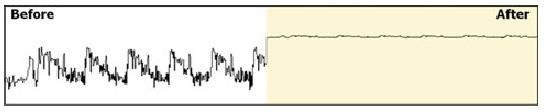
\includegraphics[width=90mm,height=25mm]{images/cri2.jpg}
	\end{center}
The previous pictures do not appear with Paul Kocher's kind authorization. 

\item \textbf{\textit{Noise :}} 
this method consist in the 'random' augmentation the consumption of chip, 
like the previous method this method makes information more difficult to extract.

\begin{itemize}
	\item[] \lokiquote{eprint-2000-hijningen}
\end{itemize}
	\begin{center}
		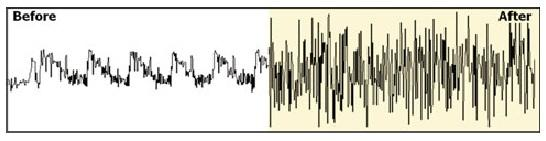
\includegraphics[width=90mm,height=25mm]{images/cri.jpg}
	\end{center}
	
\end{itemize}
All this method can be used in parallel in order to limit the power of the attacker, 
moreover those method can be used in addition of a protected implementation of the 
algorithm to be protected.

	    		\newpage
\subsection{The Transforming Masking method}
\label{The_Transforming_Masking_Method}


Here is presented in detail for the DES algorithm an important counter-measure, 
called Transformed Masking Method presented 
\footnote{Patterned and deprecated countermeasure !!}
by M-L.Akkar and C.Giraud at the CHES'2001 \nocite{ches-2001}
\cite{phd-Giraud-2007}, 


%see also \cite{fse-2003-akkar} and
% \cite{ches-2001-akkar}.


\begin{center}
"what does prevent an programmer to effectively mask the intermediate values\\ 
by xoring the plaintext, M, with a random mask, R, without changing the cyphertext??"

the S-boxes !
\end{center}

\subsubsection{General principle}
Recall that in the NIST specification $IP$ stands for the initial 
bijection of the DES, $FP$ for the final one -inverse of the $IP$-,
$EP$ stands the compressive function (surjection) at the beginning
of the $f$-function and $P$ is the bijection of the $f$-function.

As a start, hereafter is the expression of the input of the S-boxes of the first round:
\begin{center}
$EP(M_{32-63}) \oplus K_1$
\end{center}

In the case of a mask xored to the plain-text, the linearity of almost all DES 
operations -$\oplus$, $IP$, $FP$, $E$, $P$- play a central role, in the following lines,
successively, we let the mask propagate itself till just before the S-box of 
the first round:
\begin{center}
$IP(M \oplus R)_{32-63} $\\
$EP(IP(M)_{32-63} \oplus IP(R)_{32-63}) $\\
$EP(IP(M_{32-63}) \oplus EP(IP(R)_{32-63}) \oplus K_1$
\end{center}

\textbf{Principles}

To control the mask propagation become non realist in smart card: to perform the 
reverse operation is a complete non-sense, -S-boxes perform a non reversible 
operation-, to modify Sboxes two rounds by two rounds is also an option, but not in 
smart card it can only be done at an impressive memory cost. To anticipate the
propagation of the mask, the only solution is to modify the S-box in order to 
remove the mask of its input:
\begin{center}
$SM(X)=S(X \oplus EP(IP(R)_{32-63})) \oplus somethingelse$
\end{center}
This way, we have:
\begin{itemize}
		\item The mask is not entering any S-boxes 
		\item The output of any S-boxes shall is a function of the mask
\end{itemize}

\vspace{3mm}
\textbf{Definition}:\\
Are named respectively, for $i \in [1, 16 ]$ $DesLeft_i$, $DesRight_i$, 
$SecuredLeft_i$, $SecuredRight_i$ the left and right value at the beginning 
of the round $i$ for each algorithms.

\vspace{3mm}
\textbf{Proposition}:\\


\begin{tabular}{p{6.5cm}p{11.5cm}}
$DesLeft_{1} = IP(M)_{0-31}$ & $DesLeft_2= IP(M)_{32-63} $\\
$DesRight_1 = IP(M)_{32-63} $ & $DesRight_2 = P(S(EP(M_{32-63}) \oplus K_{1})))
	\oplus IP(M)_{32-63}$
\end{tabular}
\begin{center}
$SecuredLeft_{1} = IP(M)_{0-31} \oplus IP(R)_{0-31}$\\
$SecuredRight_1 = IP(M)_{32-63} \oplus IP(R)_{32-63}$\\
\vspace{3mm}
$SecuredLeft_2= IP(M)_{0-32} \oplus IP(R)_{32-63}$\\
$SecuredRight_2 = P(S(EP(M_{32-63}) \oplus K_{1}))) \oplus P(somethingelse)
	\oplus IP(M)_{0-31} \oplus IP(R)_{0-31}$
\end{center}


\newpage
Then, an interesting relation can be viewed at the beginning of the first round:
\begin{center}
$ DesLeft_1  | DesRight_1 \oplus IP(R) = SecuredLeft_1 | SecuredRight_1 $
\end{center}
or equivalently:
\begin{center}
$\left \lbrace 
	\begin{array}{lcl} 
	DesLeft_1 \oplus IP(R)_{0-31} &=& SecuredLeft_1\\
	DesRight_1 \oplus IP(R)_{32-64} &=& SecuredRight_1
	\end{array} 
\right. $
\end{center}
\textbf{Key idea}
If the previous relation hold for all round $i$, the masked algorithm is finished!! 

To finish the construction changes have to be made so as that the previous 
to be extended to the second round. 
Using the proposition on previous page, let's take to a look 
at what happen at the end of the second round, and what should be modified so as 
the previous equations to be true for each round.

\begin{center}
	$IP(M)_{0-31} \oplus IP(R)_{0-31}$ \\
	$=$\\
	$IP(M)_{0-31} \oplus IP(R)_{32-63}$
\end{center}
\vspace{3mm}
\begin{center}
	$P(S(EP(M_{32-63}) \oplus K_{1})))\oplus IP(M)_{0-31} \oplus IP(R)_{32-63}$\\
	$=$\\
	$P(S(EP(M_{32-63}) \oplus K_{1}))) \oplus 
	IP(M)_{0-31}\oplus P(somethingelse)	 \oplus IP(R)_{0-31}$
\end{center}


From these can be deduced
\begin{itemize}
	\item The second equation
impose to verify: 
		\begin{center}
			$P(somethingelse) = IP(M)_{0-31} \oplus IP(M)_{32-63}$\\
			\textit{i.e.}\\
			$somethingelse = P^{-1}(IP(M)_{0-31} \oplus IP(M)_{32-63})$
		\end{center}
	\item The Feistel scheme of the DES algorithm have to be modified a bit: the xor
	at the end of the rounds of the Feistel scheme is followed with a xor of the value
	$IP(M)_{0-31} \oplus IP(M)_{32-63}$
\end{itemize}

Let's discoverer the solution from the author, with their much more digest standards notations.

\subsubsection{Notation}
\vspace{2mm}
Notation: following NIST DES spec, $R$ is for a  8 bytes mask, 
the following notation are required to simplify notation:
\begin{center}
$R1 = IP(R)$\\
$R2 = EP(R1_{32-63})$\\
$R3 = R1_{0-31} \oplus R1_{32-63}$
\end{center} 

The idea behind this algorithm is to mask all the intermediate values in 
such way that the cipher-text will be the same. 
The mask $R$, Xored with the main key, will be propagated during a whole round.
The algorithm is build in such a manner that the mask is not allowed to enter in the 
-non linear- S-Box, then all the mask propagation is linear and finally easily controllable.

\paragraph*{}
At the end of a round result is the same than with a normal DES execution
but Xored with always the same value : $R1$. 
To anticipate the mask's propagation and be able to control them
some evolution of the mask have to be pre-computed before the 
execution of the algorithm.


\begin{center}
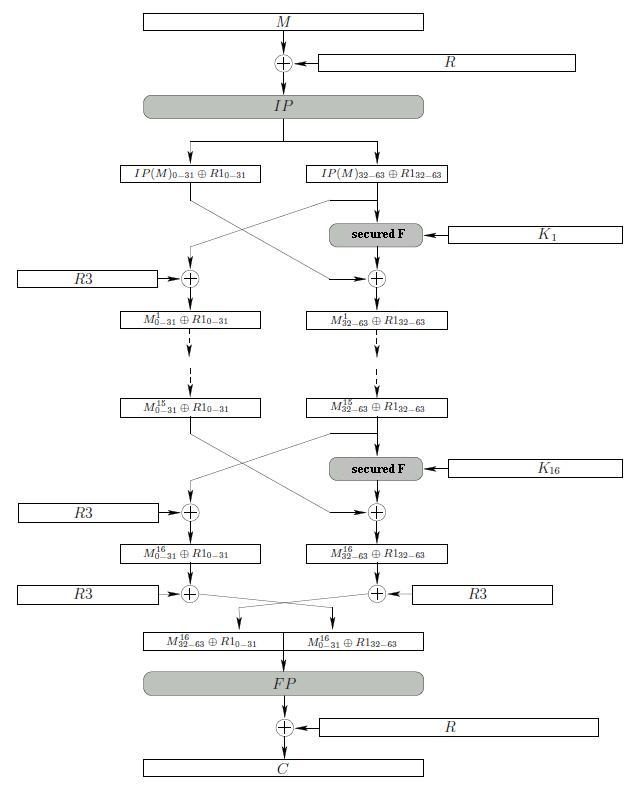
\includegraphics[scale=1.15]{images/dessecured.jpg}\\
\textit{Secured DES general scheme}
\end{center}
\newpage

\paragraph*{}
Note, that those pre-computation have to be computed in a very safe way.
Indeed, if an attacker could know those values, then immediately she/he could 
anticipate the SM-boxes for each encryption, therefore they would just launch a DPA 
attack simply changing the S boxes for the SM-boxes at each encryption.

\begin{center}
$SM(X)=S(X \oplus R2) \oplus P^{-1}( R3)$
\end{center}

\paragraph*{}
The algorithm has to be modified so as to the mask no to enter in the Sbox.
We obtain before the S-Box a intermediary value masked with $R2$. And clearly with this with 
new definition of the Sbox if the input is masked with $R_2$ 
then $R_2$ absolutely does not influence the output of those modified SMbox.


\begin{center}
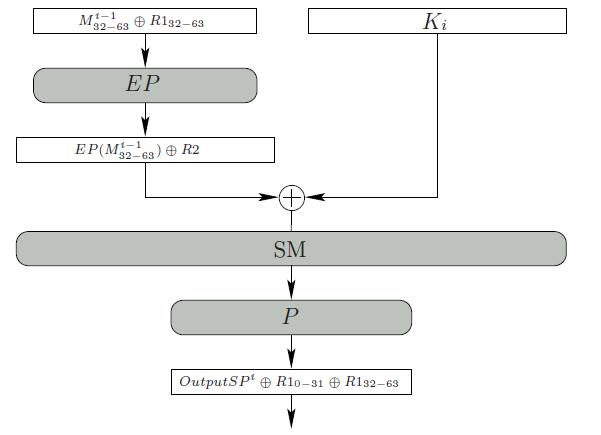
\includegraphics[width=110mm]{images/functionFsecured.jpg}\\
\textit{Secured F function}
\end{center}


\subsubsection{A round with a secured DES}

\paragraph*{} Here will be presented a complete round with the secured DES, 
and we will see that that at the end of a round the difference between a normal DES and 
the secured DES is always constant and worth $IP(R)$.
\vspace{5mm}

\textbf{Here} the letter $M$ is redefined for $M^i$ with the following convention
\begin{itemize}
\item $M^0$ stands fir the plain-text.
\item $\forall \in [1,16], \; M^i$ stand for the left|right value at the beginning
of the $i^{th}$ round.
\item $M^{17}$ stands fir the plain-text.
\end{itemize}

First of all, let's recall what is the output of this round DES algorithm, 
if we concatenate the two part, we have :
\begin{center}
$DesLeft | DesRight = M_{32-63}^i  |  P(S(EP(M_{32-63}^i) \oplus K_{i})))\oplus M_{0-31}^i$
\end{center}
Starting \footnote{In fact this lines are the induction step of a recurrence proof}
at the beginning of a round, noted $ i $, let's first calculate the 
result at the end of this round for the left side:\\
$SecuredLeft_i=M_{0-31}^i \oplus R1_{0-31}$ \\
$SecuredLeft^{'} = M_{32-63}^i \oplus R1_{32-63} \oplus R3 $ \\ 
$SecuredLeft_{i+1} = M_{32-63}^i \oplus R1_{0-31} $ \\
Secondly the same computation will be done on the right side:\\
$SecuredRight_i = M_{32-63}^i \oplus R1_{32-63} $ \\ 
$SecuredRight^{'} = EP(M_{32-63}^i) \oplus EP(R1_{32-63}) $ \\ 
$SecuredRight^{'} = EP(M_{32-63}^i) \oplus EP(R1_{32-63}) \oplus R2   $ \\ 
$SecuredRight^{'} = EP(M_{32-63}^i) \oplus K_{i} $ \\ 
$SecuredRight^{'} = 
S(EP(M_{32-63}^i) \oplus K_{i})) \oplus P^{-1}( R1_{0-31}\oplus R1_{32-63}) $ \\ 
$SecuredRight^{'} = 
P(S(EP(M_{32-63}^i) \oplus K_{i}))) \oplus R1_{0-31}\oplus R1_{32-63} $ \\ 
$SecuredRight_{i+1}= 
P(S(EP(M_{32-63}^i) \oplus K_{i})))\oplus M_{0-31}^i \oplus R1_{32-63}$ 
\vspace{5mm}
\begin{center}
$SecuredLeft_i | SecuredRight_i
	= M_{32-63}^i \oplus R1_{0-31} 
	| P(S(EP(M_{32-63}^i) \oplus K_{i})))\oplus M_{0-31}^i \oplus R1_{32-63}	$ \\
\end{center}



As a result we can see that the result, which explain that the variable obtained at the
end of a round a secured DES is the same than the one obtained by a normal DES Xored by $R1$:
\begin{center}
$SecuredLeft_i | SecuredRight_i = DesLeft_i| DesRight_i \oplus R1$\\
\end{center}

\subsubsection{Resistance against the first order DPA}
\paragraph*{} As we could see all the sensible variables of the secured DES are masked, 
moreover this boolean random mask has a uniform distribution.\\

\vspace{3mm}
With the following lemma :\\
\textbf{\textit{Let $\alpha$ $\in$ ${\mathbb{F}_2}^{n}$ an independent variable and
 $\beta$ another variable distributed uniformly on ${\mathbb{F}_2}^{n}$ and
  independent with $\alpha$. The variable $\alpha \oplus \beta$ is
 distributed uniformly and is independent with $\alpha$.}}\\
 \\
\indent Consequently we can deduct that all the variable which are manipulated
during the execution of the algorithm are uniformly distributed and
independent with the input and the key round. Thus this method resist against the
attacks of the first order DPA.


\subsubsection{Practical implementation}

In fact if the transforming masking method clearly prevent DPA attacks, 
-see before- it is not immune against side channel attacks
-see \ref{The_superposition_attack}-.
Therefore, this implementation can not be considered as secure anymore.
But in fact the "The superposition attack" can be prevented quick easily in fact:
we just have to forbid the superposition of the curve of 1st and 16th round.
This is why this Protected DES can be used at the condition to use 
two set of SM-box (one for round 1 to 8 and another for round 8 to 16).
In this configuration it is a quite popular implementation.


	    			\newpage
\section{Attacks symmetrical algs in smart cards}

\subsection{Differential Power Analysis} 
\label{Differential_Power_Analysis}

Differential Power Analysis was originally proposed by P.Kocher, 
J.Jaffe and B.June \cite{crypto-1999-kocher} in 1998.
As the power consumption is dependant from value manipulated by the algorithm 
-see section ~\ref{To model power consumption}-
this dependency can leads to an attack when a manipulated value depends only on
few bits of the secret key.

The principle of the Differential Power Analysis is to make hypothesis about those a
part of the key, to simulate the power consumption under this hypothesis and then
to perform statistical 
-see section ~\ref{Presentation of different statistical methods}-
comparisons with real curves. 

This attack require a large number of power trace, comparing to Simple Power Analysis,
but it can reveal the secret key of a device even if the recorded power traces are extremely 
noisy.
This dependency can be exploited when a variable is manipulated and only depend on few bits
of the secret key.\\
To achieve such an analysis several hypothesis have to be made:

\begin{itemize}
	\item  about the model of power consumption, this is very sensitive.
	\item  about the way that the algorithm is designed.
	\item  about the manipulated variable.
	\item  about a part of the key, noted $K_j$, on which depend the targeted variable.
\end{itemize}


Taking the example of the DES algorithm, the aim of this attack is
to reveal round key, for that it calculate 8 part of the round key, 
in order to get all the key with it. 
Once the attack is achieved, it can be launched again to calculate another part of the 
round key, and finally get the whole round key.
\vspace{3mm}

\underline{\textbf{Step 1}}: Choosing an Intermediate Result.

The first thing to do is to choose an intermediate result of the algorithm that is executed by
the attacked device, by example on the DES algorithm we can choose the output of a S-box.

So to attack an algorithm with this method you need an exemplary of this one, 
please note that we are only
interested in the value of this intermediate result so the type of 
implementation of the target algorithm
does not matter, only its design does(\textit{e.g.} where we take the intermediate value don't depend 
od the Des implementation).

This intermediate result have to be a function $f(d,k)$, called \textit{selection function},
where $k$ is a small part of the key and, most of the time, $d$ is either the plain-text
 or the cypher-text.To avoid false peaks the result of the $ f $ function must be uniformly distributed : 
\begin{center}
\textit{i.e.}  $\forall k\; \mathbb{P}(f(M_j, K_k)=1) = \frac{1}{2}$
\end{center}
 \vspace{3mm}
 
\underline{\textbf{Step 2}}: Measuring the Power Consumption.

Here we will simulate a run of the smart card.
To do so we'll need to have several text that is to be a plaintext or a cypher text,
noted $d_i$ $ \in\{ d_1, \ldots,d_D \}$ and to encrypt -or decrypt- all of this values.
For each of these encryptions -or decryptions- runs the attacker will know this value involved in the
calculation of the intermediate result chosen at step 1 and he will records the corresponding power trace.

Each of this trace, $\mathcal{C}_i$, will be noticed as following $(t_{i,j})_j=( t_{i,1}, \ldots , t_{i,T})$
for the $i^{th}$  consumption trace corresponding to $d_i$ and where $T$ is denotes the length of the trace.
The attacker measure the trace for each data block, and hence, the traces can be written as
matrix $\mathcal{T}$ of size $D \times T$.
 
It is important for DPA attacks that the measured trace are correctly aligned, because this means that
the power consumption value of each column of $\mathcal{T}$ need to be caused by the same operation. 
In order to do this two different means: to record traces on a oscilloscope with trigger signal, 
or to align curve with mathematical algorithms.


\newpage
\underline{\textbf{Step 3}}: Calculating Hypothetical Intermediate Values.

The next step of the attack is to calculate hypothetical intermediate value for every possible 
choice of $k_j$. Let's write $k_j  \in \{ k_1, \ldots, k_K \} $ where $K$ denotes the total number
of possible choice for the round key. $K$ will be 64 bits because the length of one round key is 6
bytes and for each byte there are only two possibilities $1$ or $0$. In the context of DPA
attacks, we usually refer to those elements as \textit{key hypothesis}.
Now an attacker can easily calculate $f(d_i,k_j)$.
This construction results in a matrix $\mathcal{V}$ of size $D \times K$ defined by the
following relation:
\begin{center}
$\forall (i,\;j)$ such as $1\leq i \leq D$ and $1 \leq j \leq K: v_{i,j}= f(d_i,k_j)$
\end{center}

The $j^{th}$ column of $\mathcal{V}$ contains the intermediate results that have been calculated on the key
hypothesis $k=k_j$ and as we are trying all possibility for $k$ the value used in the device is one of them.
The goal of DPA is to find this correspondence.
\vspace{3mm}

\underline{\textbf{Step 4}}: Mapping Intermediate Values to Power Consumption Values.

For this purpose, the attacker uses a technique simulation. 
The quality of this simulation strongly depends
on the knowledge of the attacker about the device. \textbf{The better this simulation 
of the attacker matches the
actual power consumption characteristics of the device, the more effective is the DPA attack.} 
We will see next how to do it. This mapping applied to the matrix 
$\mathcal{V}$ give a matrix, noticed $\mathcal{H}$ 
of the same size: $D \times K$.
\vspace{3mm}

\underline{\textbf{Step 5}}: Comparing Hypothetical to Recorded Consumption. 

Now the final step of the DPA attack can be performed:
each column of the matrix $\mathcal{H}$ is compared 
with each column of the matrix $\mathcal{T}$ with some
statistical method. This means that the attacker compares 
the Hypothetical power consumption values
of each key hypothesis with the recorded trace at every position.
The result of this comparison is a matrix $\mathcal{R}$ of size  $K \times T$,
 where each element $r_{i,j}$
contains the result of the comparison between the columns 
$h_{i}$ and $t_{j}$. The comparison is done based
on algorithms I will discuss later. \textbf{But in every algorithm, 
one thing is similar : the value $r_{i,j}$ is the
higher, the better the columns $h_{i}$ and $t_{j}$ match.} 
The key of the attacked device can hence be
revealed based on the following observation.\\
\indent The power traces correspond to the power consumption 
of the device while it executes a
cryptographic algorithm using different data inputs. 
The intermediate result that has been chosen in
\textbf{step 1} is a part of this algorithm. 
That's why the device needs to calculate the intermediate
values of the matrix $\mathcal{V}$ during the execution of the algorithm.
Consequently, also the recorded traces depend on these intermediate
values at some position.\\
\indent The hypothetical power consumption values
 in $\mathcal{H}$ have been simulated by the attacker
based on the values of the matrix $\mathcal{V}$. 
In  fact, the column of $\mathcal{H}$ and $\mathcal{T}$ are strongly related and
lead to the highest values in the matrix $\mathcal{R}$. 
All other values of $\mathcal{R}$ are low because
the other columns of  $\mathcal{H}$ and $\mathcal{T}$ are not strongly related.\\
\textbf{ The index of the line in which is the highest values of the matrix $\mathcal{R}$ is
reveals which of the key hypothesis is the more probable.}

\underline{\textbf{\textit{problem 1}}} In practice the matrix $\mathcal{R}$ 
have sometimes the same
coefficient. In this case, the attacker has usually not measured enough power traces to estimate
the relationship between the columns of  $\mathcal{H}$ and $\mathcal{T}$.
Indeed the more traces an attacker measures, the more elements 
are in the columns $\mathcal{H}$ and
 $\mathcal{T}$, and more precisely the attacker can determine the relationship between the columns.

\underline{\textbf{\textit{problem 2}}} This also implies that the more measurements are made,
the smaller relationships between the columns can be determined. 
So I had to get a good number of
measurements. On a DES implementation with no counter measure 5000 traces are 
enough to find a round key, see section ~\ref{Copy of the first attack report}.

The following diagram is illustrating the steps 3 to 5 of a DPA attack.
\newpage
\vspace{2cm}
\begin{center}
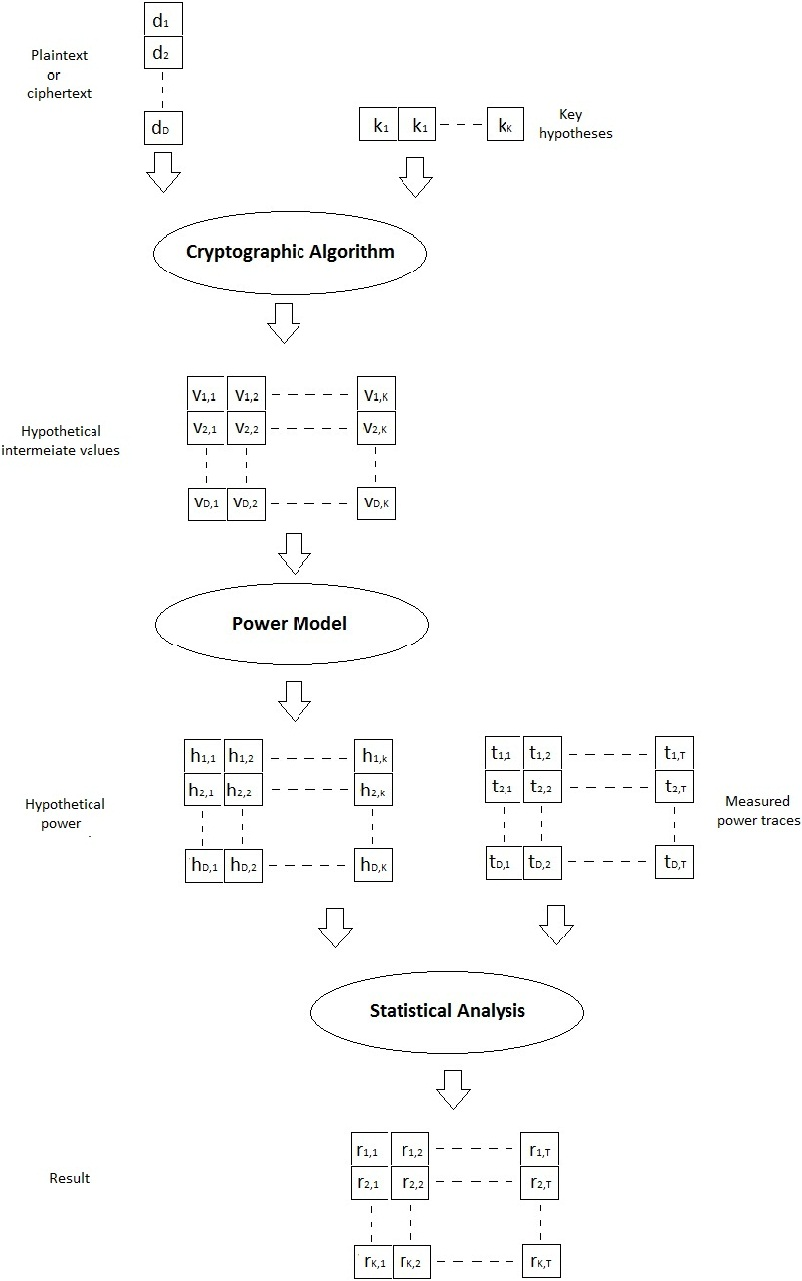
\includegraphics[width=140mm,height=185mm]{images/diagramCPA.jpg}\\
\textit{Figure 16. Schema of the DPA attack}
\end{center}

\newpage
\subsection{About the power model}
\label{About_the_power_model}

\paragraph*{}Once the $\mathcal{V}$ matrix is filled, 
it have to be transformed to $\mathcal{H}$ matrix
thanks to power consumption model, this model is crucial 
because it will depend the success of the attack.

\paragraph*{Linear models}

This model is simple and efficient because it permit to separate the consumption of 
the target electrical component (register, RAM cell, bus ) from the rest of the circuit.

For every component and at any time we have :
\begin{center}
$C =  C_{\mathit{all \; the \; circuit \; but \; the \; component}}+C_{component}$
\end{center}
Nowadays, technology CMOS is most widespread to implement the integrated circuits.
With this kind of technology, as said in \cite{phd-Messerges-2000}, the component mainly consumes
current when there is a change of state of the logical parts between two blows of clock:
the static consumption is negligible.

\paragraph*{Asymmetric model}
Let $ B = (\beta_m,...,\beta_1) $ the value that will be saved in the targeted component,
and $ A = (\alpha_m,...,\alpha_1) $ the value previously stored in this component.\\
Let also $ c_{01}^i$ and $ c_{10}^i$ be respectively the amount of currents needed to
change a bit from 0 to 1 and from 1 to 0 for the $i^{th}$ bit.
If after a clock the value of the register is set to $ B $, the consumption after the shot clock is:
\begin{center}
$C(t) = \theta+  \sum\limits_{i=1}^{m} (1-\alpha_i)\beta_i c_{01} + \alpha_i(1-\beta_i)c_{10} $
\end{center}
where $\theta$ is the electrical consumption due to others part of the circuit, and 
$ c_{01} ,\;\;c_{10}$ and $\theta$ are function of time.

\paragraph*{Symmetric models}
As proposed by Brier \cite{eprint-2003-brier} we assume that $ c_{01} = c_{10}$,
the model of power consumption, can be simplified using 
 $ d_{\mathcal{H}} $ for the Hamming distance operator to: 
\begin{center}
$C(t) = \theta(t)  + d_{\mathcal{H}}(A,B) \times c(t) $
\end{center}
where $ d_{\mathcal{H}} $ is the Hamming distance operator.\\
This model can be simplified again if assumed that the reference state A is always zero,
this model has been proposed by T.Messerges, where $ \omega_{\mathcal{H}} $ is the Hamming weight operator.
\begin{center}
$C(t) = \theta(t)  + \omega_{\mathcal{H}}(B) \times c(t)  $
\end{center}


\paragraph*{Hamming weight}
Finally the most common, for the -realistic- case that $\theta $ and $c$ are not considered as function of time:
\begin{center}
$C(t) = \omega_{\mathcal{H}}(B)   $
\end{center}
Other model exist, like the one from S.Aumonier
\nocite{ecrypt-2007} \cite{ecrypt-2007-aumonier} based on the concept of mutual
information. This model is much more general and precise that previous one, 
but on the other hand this model is much more slower.



\paragraph*{Conclusions}
\begin{itemize}
\item There are a many power model more or less close to the reality.
As always, the simpler it is, the quicker it is and of course the less precise it is.
\item Note that on Kocher's original article \cite{crypto-1999-kocher}: "mono-bit DPA"
the intermediate value is only constituted of one bit and the present section who
studied the problem of the power consumption is not relevant in this case.

\end{itemize}



	    			\newpage
\subsection{Formalization}

\subsubsection{P.Kocher's DPA mono-bit}
Hereafter is presented the original Differential Power Analysis, also called mono-bit DPA ,
which was published on P.Kocher, J.Jaffe $\&$ B.June, \lokiquote{crypto-1999-kocher}. 
This attack is called mono-bit because the $ f $ function only returns a single bit,
with such a statistical model there is no  need of power model
\textit{i.e.}: 
\begin{center}
$ \;\; f \longrightarrow  \{0,\;1\}$ \\

\vspace{1mm}
$\mathcal{H}=\mathcal{V}$
\end{center}

The principle of this statistical test is to separate traces in two classes or packet
the trace that have been collected from oscilloscope, and then to compute the means of each class.
The way used to separate those trace in two class, noted $G_0$ and  $G_1$, 
lies in the value returned by the function $f$:
\begin{center}
$G_{0,k} := \{\mathcal{C}_i  \| f(M_i,K_k)=0 \} $\\
$G_{1,k} := \{\mathcal{C}_i  \| f(M_i,K_k)=1 \} $
\end{center}
Then is computed the \textit{signal of decision the the sub key $ K_k $}:
\begin{center}
$ \Delta_{K_j}  := \overline{G_{0,k}}-  \overline{G_{1,k}}$
\end{center}

If the hypothesis made is not the good one then the distribution between the two group $G_0$ and $G_1$ are
random and after subtraction the curve of decision  is narrow to zero.
If this hypothesis is good then appears a pic at the moment when the target bit is manipulated, so,
the aim of the attacker is to find the curve with the biggest peak. 
\hspace{3mm}\\

\textbf{advantage:} Robust ans simple

\textbf{inconvenient:} false pike might occurs!\\ 
To avoid this several hypothesis have to be verified:
\begin{itemize}
	\item	the result $ f $ function must be uniformly distributed : 
$\forall k\; \mathbb{P}(f(M_j, K_k)=1) = \frac{1}{2}$
	\item The selection function must have all its output bits independent
	\item The power model have to be relevant 
\end{itemize}

\subsubsection{T-S.Messerge's DPA multi-bit}
Is presented now, an improvement of the previous statistical tools,
and called All-or-Nothing multi-bit DPA, introduced by T-S.Messerges \lokiquote{phd-Messerges-2000}. 
The main idea of this attack is to increase the distance between means with a $f$ function
returning $m$ bits instead of only one.  
\begin{center}
$ \;\; f \longrightarrow  \{0,\;1\}^m$ \\
\end{center}

To achieve this objective curves will be partitioned in three class, here are the two class
that will be used for the computation of the signal of decision:
\begin{center}
$G_{0,k} := \{  \mathcal{C}_i  \| f(M_i,K_k) = \overbrace{0\hdots0}^{m \; bits} \}$\\
$G_{1,k} := \{  \mathcal{C}_i  \| f(M_i,K_k) = \overbrace{1\hdots1}^{m \; bits} \}$\\
\end{center}
And:
\begin{center}
$G_{01,k} = \{  \mathcal{C}_i   \| \mathcal{C}_i    \notin \{ G_{0,k} \cup G_{1,k} \} \}$
\end{center}
The attacker can compute the curve of the distance between the means of each class:
\begin{center}
$ \Delta_{K_j}  := \overline{G_{0,k}}-  \overline{G_{1,k}}$
\end{center}
\textbf{advantage:}

With this method the goods pike will be $m$ times much higher than with mono bit DPA\\
\textbf{inconvenient:}

All curves of $G_{01,k} $ are lost for this attack, which clearly represent
most of them.

In order that multi-bit DPA to be still effective a compromise in the definition
of the partition have to be found, nowadays the most accepted one is: 
\begin{center}
$G_{0,k} := \{  \mathcal{C}_i  \|   \omega_{\mathcal{H}}( f(M_i,K_k) ) < m/2 \}$\\
$G_{1,k} := \{  \mathcal{C}_i  \|   \omega_{\mathcal{H}}( f(M_i,K_k) ) > m/2 \}$\\
\end{center}

\textbf{advantage:} far much relevant than All-or-nothing DPA.\\
\textbf{inconvenient:} If $m$ is odd, some curve won't be used.



\subsubsection{Correlation Power Analysis}
 The main problem with the multi-bit attack previously presented is that all the
curve are not always used when  $m$ is odd which append all the time because all kind of
architecture have an odd number of bits. This point have encourage researchers to find another 
method which would not use a partition of the curves in different classes.

Few years after the publication of  T.Messerges \cite{phd-Messerges-2000} \lokiquote{ches-2004-brier}
published a new method transforming the problem of an attack changing
the problem of detection of a difference of means for a problem of detection 
of a correlation between a set of measures and  a power consumption model.


In DPA attacks, the correlation coefficient is used to determine the linear relationship between
the $i^{th}$ column of $\mathcal{H}$ and the $j^{th}$ column of $\mathcal{T}$ for $i \in\{ 1, \ldots,K \}$
and $j \in\{ 1, \ldots,T \}$. This results in a matrix $\mathcal{R}$ of estimated correlation coefficients.
We estimate each value $r_{i,j}$ based on the D elements of the columns $h_{i}$ and $t_{j}$. So we can
rewrite with the same notation the following formula :
\begin{center}
$r_{i,j} = \frac{\sum_{d=1}^{D}(h_{d,i}-\bar{h_{i}}) . (t_{d,j}-\bar{t_{j}})}{\sqrt{\sum_{d=1}^{D
}(h_{d,i}-\bar{h_{i}})^2} . \sqrt{\sum_{d=1}^{D}(t_{d,j}-\bar{t_{j}})^2}}$
\end{center}


\textbf{advantage:} All the curve are systematically used. 





\subsubsection{Partitioning Power Analysis}

In 2006 a group of researcher composed by T-H.Le, J.Cl\'edi\`ere, C.Canovas,
 B.Robisson, C.S\'ervi\`ere and J-L \lokiquote{ches-2006-lee} presented a new method that 
was generalizing all DPA attacks in the right lineage of \cite{crypto-1999-kocher}.
In order to generalize the multi-bit DPA method, they purpose 
this method defining a large number of packets. 
The concept of multi-partitioning has been suggested by M.L-Akkar and Al, but
these authors did not formalize the concept.

For this method the hypothesis about power consumption have to be done,
so we will begin to explain this attack from the $H$ matrix that has been introduced previously.
The goal, when attacking a DES algorithm, is still to find a part of a round key associated to 
a fixed S-Box.\\
This method can be explain by the following steps :

\begin{itemize}
\item Define packets :
our selection function $f$ is returning $m$ bits, in this case we will defined $m+1$
packets defined with the previous notation :
\begin{center}$\forall \mbox{ }0 \leq j \leq m$: $G_{j,k} := \{\mathcal{C}_i,i=1..N
\|\omega_{\mathcal{H}}(f(M_i,K_k))=j \}$\\
\end{center}
\item Created average : to each packets will be associated the average of the curve 
belonging to it, that will be noted  $\overline{G_{j,k}}$.
\item Computation of the decision signal :
\begin{center}
$ \Delta_{K_j}  := \sum\limits_{j=0}^{m} \; a_{j,k}\;\; \overline{G_{j,k}}$
\end{center}
where $(a_{j,k})_{0 \leq j \leq m }$ are weight that will strongly impacts the performance
of this attack. Those weight can be dependent or not of the key assumption, in our case we have
$ a_{j,k} =  a_j $.
\end{itemize}
 Briefly, the attack works similarly as the DPA,
 the exception is after the step 5 of our DPA description. Indeed, 
we put the traces in $m$ packets, and then we calculate $ \Delta_{K_j}$.
As usually with such a signal decision the curve on which is maximum of this value will 
possibly indicate the correct hypothetical key. 
It's done for one S-box, so we have to do the same with all of them.

\textbf{\textit{Advantages :}}\\
Less curves are necessary to recover a key.\\
As the partition is more precise, the results are much more a{ches-2006-lee}\\
Strong reduction of the false and secondary peaks. The  next figure illustrate it.

\begin{center}
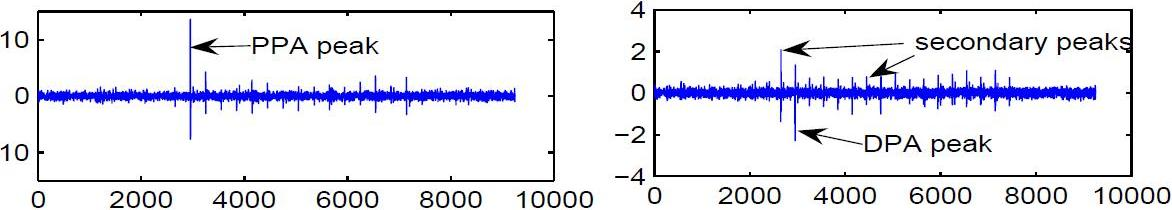
\includegraphics[width=120mm,height=22mm]{images/illustrationPPA.jpg}\\
\textit{Figure 24. Comparison between PPA and DPA for a good key hypothesis}
\end{center}

\textbf{inconvenient:}\\
In the case of $m = 2$, all curve of $G_{2} $ will not be used for the computation of $ \Delta_{K_j} $.


\subsubsection{PPA generalize all previous DPA attacks}

\textbf{1)} For specific values of the weight we are in fact defining well known attacks :\\
$\bullet$ if the values are : $a_0=-1$ and $a_4=1$ and other set to 0 it's the P.Kocker mono-bit DPA.\\
$\bullet$ if the values are :
\begin{center}
 $ a_j =\left\{ \begin{array}{ll}  -1$ if $0 \leq j < m/2 \\\;\;1$ if $m/2 \leq j \leq d\end{array} \right.$
\end{center} 
it's the P.Kocher mono-bit DPA.\\
it's the  all T.Messerges multi-bit DPA and OAN-DPA.\\
\textbf{2)} The reader can also read the demonstration which explain that the CPA
is also a particular case of PPA for some specific values of $a_j$.\\
\textbf{3)} Optimal values for weights are $(a_j)_{0 \leq j \leq m  } = \{-1,-2,0,2,1\}$, 
this set of weights is maximizing the Signal Noise Ratio for the linear model of power consumption. 
See \lokiquote{asiacs-2008-Lee}.

\subsubsection{Maximum of probability}
This method was invented by R.Bevan and E.Knudsen [1]. This method takes into account
 what appends when the amount of current to pass a bit from 0 to 1 is different from that needed to pass a
  bit from 1 to 0. 
With the model of consumption we have :
\begin{center}
$\mathcal{C}_{i}=\sum_{k=1}^{p}\lambda_{ki} \theta_{k} + w_{i}$,
\end{center}
which $\theta_{k}$ is the parameters of the consumption model and p the number of parameters.\\
For $N$ different consumption measures, we have the matrix relation :
\begin{center}
\begin{displaymath}
\mathcal{C}=
\left(\begin{array}{ccc}
\mathcal{C}_{1} \\
\vdots \\
\mathcal{C}_{N} \\
\end{array}\right)
=
\left( \begin{array}{cccc}
\lambda_{1,1} & \lambda_{2,1} & \ldots & \lambda_{p,1} \\
\vdots        & \vdots        &        & \vdots \\
\lambda_{1,N} & \lambda_{2,N} & \ldots & \lambda_{p,N}\\
\end{array} \right) 
\left( \begin{array}{ccc}
\theta_{1} \\
\vdots \\
\theta_{N} \\
\end{array} \right)
+
\left( \begin{array}{ccc}
w_{1} \\
\vdots \\
w_{N} \\
\end{array} \right)
\end{displaymath}
\end{center}

with this notation the attacker will keep the key which maximize the following relation :
\begin{center}
$L_{K_{j}}=\frac{N}{2} ( ln({}^t \! \mathcal{C} . \mathcal{C} - \frac{1}{N}(\sum_{i=1}^{N}\mathcal{C}_{i})^2)
- ln({}^t \! \mathcal{C} . \mathcal{C} -ln({}^t \! \mathcal{C} . \lambda_{K_{j}}.( {}^t \! \lambda_{K_{j}}.
\lambda_{K_{j}})^{-1} . {}^t \! \lambda_{K_{j}}.\mathcal{C}))$
\end{center}

\newpage
\subsection{Compare those methods}
Reference
The two references could be :
\begin{itemize}
	\item In 2004 Regis Bevan PhD in \lokiquote{phd-Bevan-2004}: are compared mono-bit, 'All or Nothing multi bit DPA', multi bit DPA and CPA.
	\item In 2011 Julien Doget's article \lokiquote{jce-2011-doget} : much more comparison, ultimately clear notations.
\end{itemize} 

Hereafter picture beeing taken from the excellent article of Julien Doget, 
a comparison in term of efficiency between many statistical methods. 
Note that mono bit DPA return bit of key whereas the other return 6.

\begin{center}
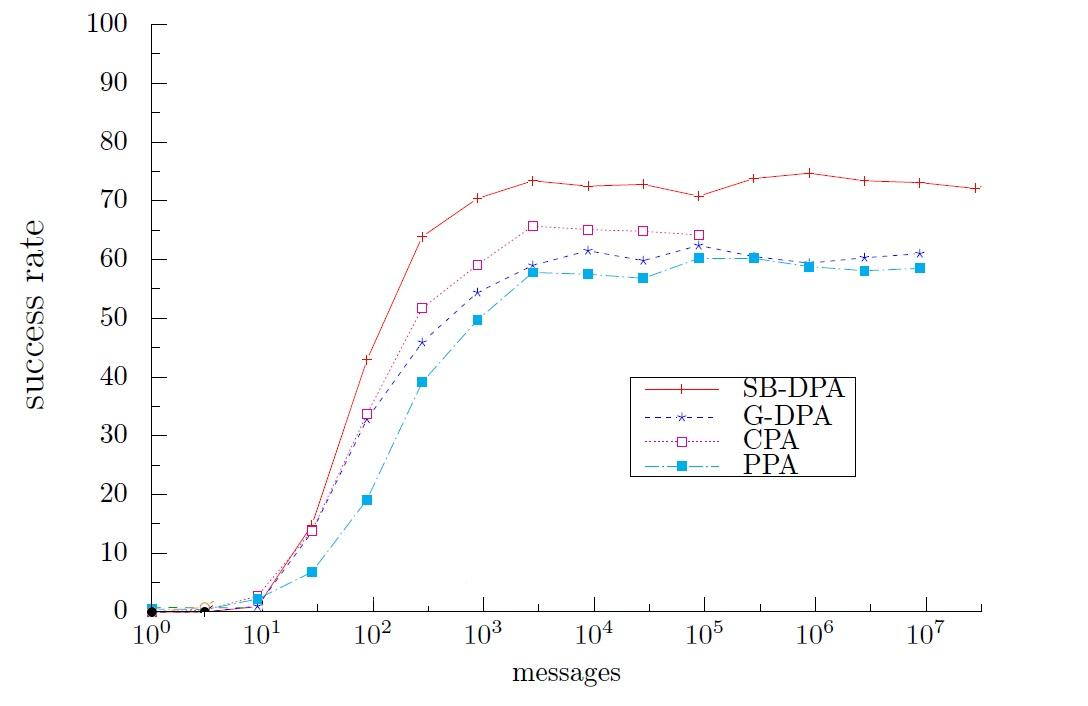
\includegraphics[width=140mm,height=95mm]{images/compare.jpg}\\
\end{center}

	    			\newpage
\subsection{High Order DPA attacks}
\label{High_Order_DPA_attacks}


See \cite{phd-Giraud-2007}, his PhD study in detail this attack on AES, 
and see also the original article \cite{fse-2003-akkar} and \cite{ches-2001-akkar}.

We saw that testing hypothesis about a manipulated variable depending on a part of
the key, part small enough so that a brute force search could be 
undertaken, could lead to reveal the used secret key.

We saw afterwards, that this kind of threat can be prevented, simply by breaking 
the link between the manipulated value and the power consumption: this means
practically that no attacker shall be able to anticipated any sensitive manipulated 
value by technique such as masking.

In fact this kind of countermeasure can be bypassed, by another class of side 
channel attack generalization of the DPA seen previously. Instead of doing hypothesis
on one manipulated variable, those Hight Order DPA attacks do hypothesis one multiple 
intermediate value.

      \begin{figure}[!h]
        \centering
        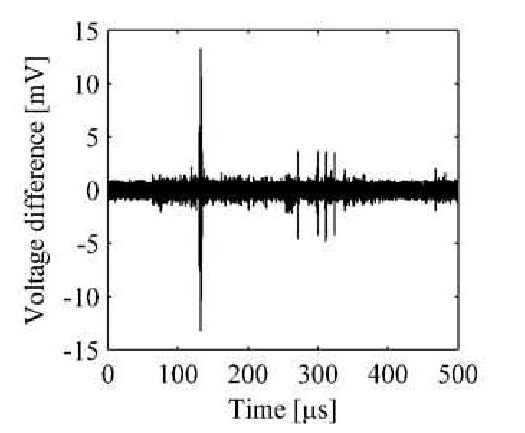
\includegraphics[width=10cm,height=3cm]{images/dpa_result.png}
        \caption{Successful DPA attack}
      \end{figure}	
      
More than the number of sub key hypothesis -which is squared for HODPA square- the 
main difference between DPA and -true- HODPA is that DPA attack 
target one variable manipulated in moment in time, $\tau$ whereas HODPA 
target multiple variable manipulate at moment in time $\tau_1$, $\tau_2$, ...

      \begin{figure}[!h]
        \centering
		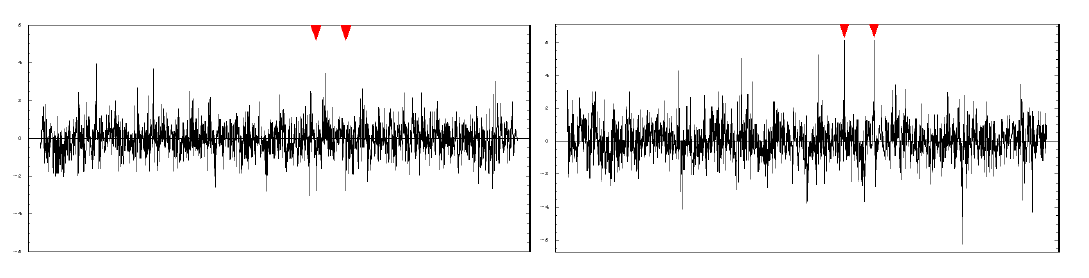
\includegraphics[width=14cm,height=3cm]{images/hodpa_result.png}
		\caption{Unsuccessful \textit{vs} successful HODPA attack}
      \end{figure}	

\subsubsection{A particular case: The superposition attack}
\label{The_superposition_attack}

The superposition attack proposed by M-L.Akkar and L.Goubin against their own implementation 
' the Transforming masking method', see \ref{The_Transforming_Masking_Method}.
This is a second order DPA attack in theory because the selection function used is function of two distinct 
sub-keys. But in practice, it is nearly as simple as an usual DPA attack. '\#1.333 HODPA'
\vspace{3mm}
 
The idea is as following: in a second order DPA attack, the most
difficult thing is to localize the time when the precise needed values are manipulated,
but on the contrary, localizing a whole DES round is often quite easy.
So instead of correlating precise parts of the consumption traces, the attacker
will just correlate the whole trace of the first and the last round.
\vspace{3mm}

The main idea is to perform a front attack with a plain-text $M$, making an hypothesis
on a part of $K_1$, in the same time to perform a back-end attack with a cypher text $C$,
making another hypothesis on a part of $K_16$.
For one S-Box there will have 4096 possibilities for a sub-key hypothesis.\\
As we can see, by example with picture \textit{26} , every output of SM-Box are masked 
with a value depending on the main mask,
the thing that allow an attack to be possible is the fact that the value
$P^{-1}( R1_{0-31}\oplus R1_{32-63})$ is always the same.

Then  we have:
\begin{center}
$T =    S(EP(IP^{-1}(C)_{32-63}) \oplus K_{16}) \oplus P^{-1}(IP(R)_{32-63} \oplus IP(R)_{0-31})) $

$\oplus S(E(IP(M)_{32-63}) \oplus K_1) \oplus P^{-1}(IP(R)_{32-63} \oplus IP(R)_{0-31})))$\\  
\end{center}
\begin{center}
$T = S(E(IP^{-1}(C)_{32-63}) \oplus K_{16}) \oplus S(E(IP(M)_{32-63}) \oplus K_1)$
\end{center}

Key idea : that the value $T$ does not depend on the random masking value.

On the next page is explained the different step of the algorithm, one can note that 
the presented version, taken from \cite{fse-2003-akkar}, is a mono-bit DPA attack and 
that T.Messerge's multi-bit attack, would also work just like a CPA attack.


			\begin{algorithm}[h]
				\KwIn{Curves resulting of the addition of traces from round 1 and 16 }
				$y \leftarrow 1$	\;	
					\For{$i=0 \mbox{ } j<64 \mbox{ }i++ $ }{			 
						 \For{$j=0 \mbox{ } j<64 \mbox{ }j++ $ }{			 
							 \For{ All the Curves }{			 
					Separate the curves in two packets depending on one bit of the part of $T$ which is
					corresponding to the attacked S-box and assuming that the part of $K_1$ and $K_{16}$
					corresponding to the attacked S-box are $i$ and $j$.\\
					Average and subtract the separated curves.
							} 
						} 	
					}
					Choose the value of $i$ and $j$ where the greatest peak appears.\\
					Check the coherency the $i$ and $j$ has to be compatible. 	\;							 
				\Return{$ i,j $}\;
				\caption{Superposition Attack on S-boxes}
			\end{algorithm}

Note that this algorithm requires as an input to sum two round of a DES, if there is 
a problem of alignment this will dangerously compromise the attack.


\newpage
\subsubsection{General HODPA}
\label{eneral_HODPA}

	
In classical DPA attack once that the trace have been processed to remove noise, aligned and so on
it sure that if an attack was launched on those traces then peaks would occurred exactly when the 
targeted variable is manipulated.  This is assuming few hypothesis:
\begin{itemize}
	\item power consumption was measured while the targeted variable was manipulated
	\item a relevant power model is available and compatible with the countermeasure.
\end{itemize}

In HODPA as multiple manipulate variable are targeted, and as those variables
are manipulated at different moment in time, let's say $\tau_1$ and $\tau_2$,  
it wouldn't make any sense to launch this attack on recorded trace, 
the trace to be process align and then separate in packet are in 
fact traces that have not been recorded.
\vspace{3mm}


$\mathcal{T}_i(t)$, attacked traces, for HODPA targeting two variables,
in function of $\mathcal{C}_i(t)$ the recorded trace:

\begin{center}
$ \mathcal{T}_i(t) = \mathcal{C}_i(t)  -  \mathcal{C}_i(t + \tau_2 -\tau_1) $
\end{center}

This way for $t = \tau_1$ the fist contribution of the attacked curve 
$\mathcal{C}_i(t) $ will give pike relative to the manipulation of the first variable while at the 
the second contribution of the attacked curve $ \mathcal{C}_i(t + \tau_2 -\tau_1)$ 
will give pike relative to the manipulation of the second variable.
Morality: with such a trace $\mathcal{T}_i(t)$, peak will pop up at $t =\tau_1$
revealing that the the two targeted variable are manipulated at $\tau_1$ and $\tau_2$, .
Note that on a natural case, $\tau_2 -\tau_1$ is not known , moreover  $\tau_2$  and $\tau_1$,
then all the possibility would have to be tested .... Huge increase of the complexity.




	    	\chapter{Asymmetric encryption}
	    		\newpage 
\section{RSA: description}
\label{Asymmetricalintro}

\subsection{References}

More in \cite{book-1996-menezes} :
\begin{itemize} 
	\item fundamentals, chapter 2: "number theory", "finite fileds", "abstract algebra"
	\item Asymetrical PKCS, chapter 8: "RSA public key encryption"
\end{itemize}

We recall the classic notation: $\mathbb{Z} = \{ ...,\;-2,\;-1,\;0,\;1,\;2,\;...\}$,
 for this document all the computation will take place in the following 'set':
If $n$ is a positive integer:
\begin{center}
$\mathbb{Z}/{n \mathbb{Z}} = \{0,\;,...,\;n-1\}$
\end{center} 
where classical addition, subtraction, and multiplication are defined just like in $\mathbb{Z}$
with the amendment that results must be in the set $\mathbb{Z}/{n \mathbb{Z}}$.
\subsection{Modular arithmetic} 

\vspace{4mm}
\begin{mydef}
$x \in \mathbb{Z}/{n \mathbb{Z}}$ is said to be invertible in the ring 
$\mathbb{Z}/{n \mathbb{Z}}$\\
if there exist $y \in \mathbb{Z}/{n \mathbb{Z}}$
such that $x*y=1$ in $\mathbb{Z}/{n \mathbb{Z}}$ 
\end{mydef}


Notation:\\
the set of invertible of $\mathbb{Z}/{n \mathbb{Z}}$ is noted $ ( \mathbb{Z}/{n \mathbb{Z}} ) ^\times$\\
the number of invertible of $\mathbb{Z}/{n \mathbb{Z}}$ is noted $\phi(n)$

\begin{mydef}
	A prime number is a natural number that has exactly two distinct natural number divisors: 1 and itself.
\end{mydef}
\begin{mydef}
	Two integers a and b are said to be co-prime if they have no common positive factor other than 1.
\end{mydef}
\begin{mythm}
	If $ n = p*q $ where $p$ and $q$ are prime numbers,\\
	Then $\phi(n) = (p-1)(q-1)$
\end{mythm}
\begin{mythm}{Euler's theorem}\\
	\label{Euler's theorem}
	If $x \in \mathbb{Z}/{n \mathbb{Z}}$ with $x$ co-primewith $n$,
	then $x^{\phi(n)}=1$ in the set $\mathbb{Z}/{n \mathbb{Z}}$
\end{mythm}


RSA stands for Ronald Rivest, Adi Shamir et Leonard Adleman who first publicly described it in 1976, but it might be true that it was known before by some governmental agencies.
\subsection*{Keys generation}
\begin{itemize}
\item Choose two distinct, 'same size' big prime numbers $p$ and $q$.
\item Compute $n = pq$. It define the set $\mathbb{Z}/{n \mathbb{Z}}$ where all the computation will take place.
\item Compute $ \phi(n)= (p-1)(q-1)$ it must be kept secret. 
\item Compute $\lambda(n) = lcm(p-1, q-1)$. 
\item Choose an integer $e$ such that $1 < e < \lambda(n)$ and $gcd(e, \lambda(n)) = 1$; i.e., $e$ and $\lambda(n)$ are co-prime.
	\footnote{here $\lambda$ is  function, many description ignore this part as most of the time Euler's function will provide the same result ... but not always, see
		\href{https://en.wikipedia.org/wiki/Carmichael_function}{Carmichael's totient}}. Note that implies $\forall x \in \mathbb{Z}/{n \mathbb{Z}} \quad x^{e \times d} =1 $, then $(n, e)$ is released as the public key exponent.
\item Compute $d$ the modular multiplicative inverse of $e$ in $\mathbb{Z}/{\phi(n) \mathbb{Z}}$.
This is often computed using the extended Euclidean algorithm.
$d$ is kept secret this is the private key of the crytposystem.
\end{itemize}
$(n,e)$ is the published private key\\
$(n,d)$ is the private key: it suffice to recover any original message, however
\begin{center}
	$d,\lambda(n),\phi(n),p,q$ must be kept secret as any of these value is enough to find $d$	
\end{center}


\subsection*{Encryption/Decryption}
	Alice transmits publishes her public key $(n,e)$ and keeps the private key secret.\\
	Bob then wishes to send message $M$ to Alice.
	He first turns $M$ into an integer $0 < m < n$ by using an agreed-upon reversible 
	protocol known as a padding scheme.	He then computes the cipher-text $c$ corresponding to:
	\begin{center}
		$c = m^e$ mod $n$\\
	\end{center}
	Alice can recover $ m$ from $c$ by using her private key exponent d by the following computation:
	\begin{center}
		$m = c^d$ mod $n$
	\end{center}
	Given $m$, she can recover the original message $M$ by reversing the padding scheme.
	
	\paragraph*{Sign/verify} Alice wants to transmit a unencrypted message $m$ 
	and to sign too, then she concatenates her 	message with the same message 
	encrypt with her private-key then everyone can verify encrypting the signature
	that was with the message to which it is concatenate.

	\paragraph*{Cypher/Sign} 
	Depending on which exponent is used to do the operation on a public data, this algorithm can either sign a data and everyone can verify it or allow everyone to cypher a data to the private key's recipient.

\subsection*{RSA example}\mbox{}\\
Key generation: \vspace{-5mm}
	\begin{itemize}
		\item we choose $p = 61$ and $q = 53 $.
		\item $n= p*q=  3233$ is computed.
		\item $\phi(n)= \phi(p*q)=\phi(p)*\phi(q)=(p-1)*(q-1)=  3120$
		\item Choosing a number for $e$ leaves you with a single check: 
		that $e$ is not a divisor of $3120$. $e = 17$.\\
		\item Compute $d$ such that it is the modular multiplicative inverse of $e$ modulo $\phi(n)$: 
		$d = 2753$\\
		since $17 * 2753 = 46801$ and $46801$ mod $3120 = 1$, this is the correct answer.
	\end{itemize}
	\begin{center}
		The public key is $(n = 3233, e = 17)$.\\
		The private key is $(n = 3233, d = 2753)$. \\	
	\end{center}
Encryption/decryption: \vspace{-5mm}
	\begin{itemize}
		\item Encryption: let's assume that $m = 65$,\\
		$c = m^e$ mod $n = 65^{17}$ mod $3233 = 2790$
		\item Decryption: we have received $c = 2790$,\\
		$m = c^d$ mod $n = 2790^{3120}$ mod $3233 = 65$
	\end{itemize}


\subsection*{RSA example CRT version}
 	As $n=pq$ exponentiations mod $p$ and mod $q$ will always be faster than exponentiation mod $n$,
 	moreover a link (an isomorphism!) exists between  $\mathbb{Z}/{p \mathbb{Z}} \times  \mathbb{Z}/{q \mathbb{Z}}$ and  $\mathbb{Z}/{n \mathbb{Z}}$
 	via the Chinese remainder theorem -CRT-. Hereafter is an example\\
 	We already have chosen $p=61$, $q=53$, $e=17$, $d=2753$\\
Encryption: starting from $m=65$ \vspace{-5mm}
	\begin{itemize}
		\item $m_p= m \mod p=4$
		\item $m_q= m \mod q=12$
		\item $\phi(p)=p-1=60$
		\item $\phi(q)=q-1=52$
		\item $e_p= d \mod \phi(p)=17$
		\item $e_q= d \mod \phi(q)=17$
		\item $s_p={m_p}^{e_p} \mod p=45$
		\item $s_q={m_q}^{e_q} \mod q=34$
		\item $p_{-1}= p^{-1} \mod q=38$
		\item $q_{-1}= q^{-1} \mod p=20$
		\item $s=s_p*q*q_{-1} + s_q*p*p_{-1} \mod n=2790$
	\end{itemize}
Decryption: starting from $s=2790$ \vspace{-5mm}
	\begin{itemize}
		\item $s_p= s \mod p=45$
		\item $s_q= s \mod q=34$
		\item $\phi(p)=p-1=60$
		\item $\phi(q)=q-1=52$
		\item $d_p= d \mod \phi(p)=53$
		\item $d_q= d \mod \phi(q)=49$
		\item $m_p={s_p}^{d_p} \mod p=4$
		\item $m_q={s_q}^{d_q} \mod q=12$
		\item $p_{-1}= p^{-1} \mod q=38$
		\item $q_{-1}= q^{-1} \mod p=20$
		\item $m=m_p*q*q_{-1} + m_q*p*p_{-1} \mod n=65$
	\end{itemize}

\paragraph*{Remark on CRT implementation} 
	Obviously there are more computations involved in CRT version, but they are much faster.

	The computation involving the more resources is exponentiation with the CRT version the speed-up is a time 4.

	Additionally many operation can be precomputed once and for all like
	$e_p,e_q,p_{-1},q_{-1}$ and stored to be reused each time

	Finally the last formula Gauss's recombination is not used in practice.

	In the end CRT is a best practice, because of the speed up.

\subsection*{Correctness}\
	We have to prove that $ (m^e)^d $ mod $ n =m $: \\
	first let's remark that the definition of $d$ implies that 
	$ed=1+k \phi(n)$ where $k$ is an integer.\\
	$ (m^e)^d $ mod $n = m^{e \times d} \, \mod  n $\\
	$ (m^e)^d $ mod $ n = m^{1+k \phi(n)} \mod n $\\
	$ (m^e)^d $ mod $ n = m \times m^({\phi(n)})^k \mod n $\\
	Assuming that $m$ is co-prime to $n$ we can applies Euler's theorem and:
	$ (m^e)^d $ mod $ n = m 1^k \mod n $\\
	$ (m^e)^d $ mod $ n = m   \mod  n $ 
	
	Please note that if $m$ is not relatively prime to $n$, Euler's theorem can not be applied and further considerations are mandatory.

\newpage
\subsection{Cryptographic problems}

Asymmetrical cryptography rely on Complexity Theory which is a branch
of the theory of computation in theoretical computer science and mathematics 
that focuses on classifying computational problems according to their inherent 
difficulty, and relating those classes to each other.

What interests cryptographer very asymmetrical problems : problems very easy to
do in a way but extremely difficult to do in the other way.

A typical example of asymmetrical problem is the factorization: 
given two numbers it is very easy to compute their product 
but, asymptotically, it is extremely difficult to factorize a product. 
This in this precise problem with two primes factor that relies the security of RSA.\\ 
\textit{Definition:}
\begin{itemize}
\item Let $n$ product of two prime numbers $p$ and $q$ what is called the factorisation problem is:
knowing $n$ find $p$ and $q$ such that $n = pq$.
\item To break RSA means if  $(n,e)$ be a RSA public key to find the private key: 
$d$ such that $e d = 1$ mod $\phi(n)$.
\end{itemize}
Propositions:

%Knowing $\phi(n)$ is equivalent to know the factorisation of $n$.\\
Knowing a RSA public key and a RSA private key then we can know the factorization of $n$. 
And we saw that thanks to the extended Euclidean algorithm if we know a factorization of $n$ 
it is easy to find the private key.
\begin{center}
\textbf{So, breaking RSA is equivalent to solve the factorization problem.}
\end{center}



\paragraph*{The RSA problem}

Definition:

Let $(n,e)$ be a RSA public key what is called the RSA problem is :
\begin{center}
\textbf{knowing $c$ co-prime to $n$, to find $m$ such that $c = m^e$ mod $n$.}
\end{center}
It means to be able to find one plain-text from it's cypher-text, 
without finding the private key.

The following assertion is not proven yet:\\
If someone can resolve the RSA problem many times then he break RSA. 
And then maybe that the RSA problem is easier than the factorization problem.



	    		\newpage
\section{Asymmetrical implementation in smart cards}
\label{Asymmetrical_implementation_in_smart_cards}

\textit{Notation:}
In the following part of the text:
\begin{itemize}
	\item $( \mathbb{G},\; \times )$ is a commutative group
	\item $x$, $y$ and $z$ three elements belonging to this group
	\item $n$ an positive integer
	\item $ln_b(x)$ is the Neperian logarithm in base $b$ of $x$ 
		\textit{i.e.} $ln_b(x)= ln(x)/ln(b)$ 
\end{itemize}
Without an explicit mention those algorithms work for every commutative group
\footnote{On of the first property of commutative, or Abelian groups, is to give a sense to Binomial theorem and its generalization (multinomial theorem)} $ \mathbb{G} $.
Note that is was not always possible to say 'the improvement of this algorithm
lies in the multiplication only', so be careful. By example the Infineon technologies ZDN algorithm is an algorithm improving at the same time, multiplication and reduction.
\vspace{5mm}



			
	    			\subsection{Number representations}
\label{RSA_representation}

This section will be mainly dedicated to the different ways to represent 
numbers \textit{i.e.} integers or relative numbers. Plan id the following:
\begin{itemize}
	\item  Classical $b$-arry representations
	\item  Some binary representations
	\item  Non adjacent representations
\end{itemize}
AIM: Change the representation of a an integers or relative numbers for a new one.
What will be obtained might be a less simple, or might requires  more amount of digits but will be but richer in term of algebraic/computational proprieties(s).\\

\noindent
	\begin{mydef}{Canonical vs Non-Canonical representation}
		\begin{itemize}
			\item 'canonical' is used to indicate a standard way to represent a 
			mathematical object under the form of a mathematical expression.
    		This a particular convention that was accepted as standard among 
    		an important number of possible conventions. 
			\item 'non-canonical' by opposition means that the convention used to 
			to represent a mathematical object under the form of a mathematical 
			expression is not he standard one, therefore this expression is 
			meaningless unless convention to which it is referring is specified.
		\end{itemize}
    \end{mydef}		

Example:\\
In geometry, the canonical way to represent objects is referring to a Cartesian 
coordinate system system and no-one wonder what type of mathematical object 
represent the following expression $(x-h)^2+(y-k)^2= \rho^2$, 
(circle centered on $(h,k)$ and of radius $|\rho|$).
\newpage
\subsubsection{Mathematical notation}
Two way to interpret Euclidean division: \\

\begin{mydef}{Euclidean division:} \\
	Given $a,b $ positive integers there exist a unique couple of integers $ (q,r)$ \\
	such that decompose uniquely $a$ in the famous Euclidean form.\\
	\textit{i.e.} Given $a,b \in \mathbb{N}$ $\exists! (q,r) \in \mathbb{N}^2$, such that:
	\begin{center}
			$a = b \times q + r$ with $0\leq r <b$\\
	\end{center}
\end{mydef}		 
		As a consequence each number, can be decomposed the following way:\\
		$n = 2^k \times b  + r$ with $0 \leq r <2^{k-1}$. \\
		$n = 2^k \times b + r$ with $-2^{k-1}<r \leq 2^{k-1}$ \\\\
		The first equality is the canonical one, it allows representation in any $b$-basis with positive digits, whereas the second one, not canonical, enable representations in any binary basis with positive and negative digits but with 
		smaller absolute values -Useful for ECC, RSA with NAF exponent-.\\\\
		Iterating the division process on $a$ from the highest power of $b$ to 0, a link is naturally created between polynomial in $b$ and representation in basis $b$.\\\\
\textbf{Possible properties of $b$-basis representations}\\
* position relativity: representation in which the localization of a digit matters\\
* completeness for $\mathbb{S}$: each element of a set of number $\mathbb{S}$ can be represented\\
* uniqueness for $\mathbb{S}$: each element of $\mathbb{S}$ admits only one representative.\\
* homogeneity: representation in which all operations are performed in the same way.\\
* optimality: representation in which a propriety is minimized -Length, Hamming weight, many others-
among a larger family of representation.

Remarks:\\
* For positional representation system:
the basis is always written the same manner, $10$, consequence of link between $b$-arry representation/polynomial expansion of variable $b$:\\
$ 10 = 10_{10} $, $ 2 = 10_{2} $, $ b = 10_{b} $, $ -b = 10_{-b} $ \\
* Interesting properties are the span and shape of $\mathbb{S}$:\\
is this including negative number? is this a perfect, quite, strongly not, symmetrical span?\\
* In the following section, we always have $a \in \mathbb{S}$

Notation: \\
* $b \in \mathbb{N}^*$, basis will be $b$ or $-b$ \\
* $ \mathcal{D} $ is the digit space.\\
* $t$ number of bits of the considered architecture

\subsubsection{Classical $b$-arry representations}
Here are approached some classical general representations.

\begin{itemize}
	\item Unary notation: representation with $b=1$, \textit{aka} 'Peano Unary system'.\\
		Simplest way to represent integers numbers...\\
		For that representation to include $0$ we impose digit space to admits two elements\\
		$/!\backslash$ Formal -but non consistent with the general one- scripture
		\begin{small}
			\begin{center}	
		$ a_{1} = \sum \limits_{i=0}^{t-1} a_i$ and $\forall i, a_i \in \mathcal{D} =\{0,1\}$ 	
			\end{center}
		\end{small}
		* completeness for $\mathbb{S} = \llbracket 0, t \rrbracket$ \\
		* no uniqueness neither a positional system\\
		* the value 0 can only be implicitly represented by an empty digit string\\
		* addition is in fact concatenation, homogeneous\\
		
	\item $b$-arry notation: general canonical representation in base $b$, for $b \in \mathbb{N} \backslash \{0,1\} $ :\\	
		starting from the least significant digit, number is obtained via a polynomial in $b$ which coefficients are the digits of the number representative.
		\begin{small}
			\begin{center}	
				$ a_{b} = \sum \limits_{i=0}^{t-1} a_i \times b^i$ 
				and $\forall i, a_i \in	\mathcal{D} = \{0, ..., b-1\}$		
			\end{center}
		\end{small}	
		% A = (b-1) * sum b^i,i=0,t-1 = (b-1) * B, and 
		% B = (b^t-1)/(b-1)
		* unique representation for $\mathbb{S} =\llbracket 0, b^{t}-1\rrbracket$\\
		* homogeneity

	\item Signed $b$-arry notation: representation in base $b \in \mathbb{N} \backslash \{0,1\} $, \textit{aka} 'Sign and Magnitude  in base $b$'
		\begin{small}
			\begin{center}	
					$ a_{b,signed} = a_t \sum \limits_{i=0}^{t-1} a_i \times b^i$ and $\forall i, 
					a_i \in \mathcal{D} = \{0, ..., b-1\}$ 		
			\end{center}
		\end{small}	
		% from previous one
		* completeness for  $\mathbb{S}=\llbracket 1-b^{t-1}, b^{t-1}-1\rrbracket$ \\
		* non unique representation + 0 and -0\\
		* non homogeneous system ! \\
		* Simple to implement \\  
		* Symmetrical span
			
	\item Nega $b$-arry notation: canonical representation in base $-b$ 
		for $b \in \mathbb{N} \backslash \{0,1\} $ : 
		\begin{small}
			\begin{center}	
					$ a_{-b} = \sum \limits_{i=0}^{t-1} a_i \times (-b)^i$ 
					and $\forall i, a_i \in \mathcal{D}=\{0, .., b-1\}$ 		
			\end{center}
		\end{small}	
		% AM = (b-1) * sum (-b)^i, i=0,t-1   and i \in 2N = (b-1) * BM
		% BM = 		   sum (-b)^i, i=0,t-2   and i \in 2N
		% BM = 		   sum   b^(2i), i=0, t/2-1 = (b^t-1)/(b^2-1)
		% AM = (b-1) * (b^t-1)/(b^2-1)
		%
		% Bm =         sum (-b)^i, i=0,t-1   and i \in 2N+1
		% Bm = 		   sum (-b)^i, i=1,t-1   and i \in 2N+1
		% Bm =    -b * sum b^(2i), i=0, t/2-1
		% Am =    -b * (b-1) * (b^t-1)(b^2-1)
		%
		%$ -b \frac{b^t-1}{b+1}, \frac{b^t-1}{b+1}$	
		* completeness for a $\mathbb{S} = \llbracket -b \frac{b^t-1}{b+1}, \frac{b^t-1}{b+1}\rrbracket $ \\
		* completeness for $\mathbb{S}$ without bit sign ! \\
		* uniqueness for $\mathbb{S}$ \\
		* although arithmetic operations are more complicated, homogeneity of operations ! \\
		* $/!\backslash \hspace{1mm} \mathbb{S}$ not centered on 0, strongly asymmetrical span $\hspace{1mm} /!\backslash$

	\item  One's complement in base $b$ 
		\begin{small}
			\begin{center}	
					$ a_{b,1*} = (b^{t}-1)_b-a_b$ 
					% a = (b^t-1) - a_{b,1*}	
			\end{center}
		\end{small}	
		* except MSB, each bit is a power of $b$
	\item  Two's complement in base $b$ 
		\begin{small}
			\begin{center}	
					$ a_{b,2*} = b^{t}_b-a_b$ 				
					% a = b^t - a_{b,2*}
			\end{center}
		\end{small}	
		* except MSB, each bit is a power of $b$, except for the most significant bit,\\
		whose weight is the negative of the corresponding power of $b$.
\end{itemize}

\subsubsection{Some binary representations}
	\begin{itemize}	
		\item  Binary notation: canonical representation base 2:
		\begin{small}
			\begin{center}	
					$  a_{2}  =  \sum \limits_{i=0}^{t-1} a_i \times 2^i$ 
					and $\forall i, a_i \in \mathcal{D}= \{0,1\}$		
			\end{center}
		\end{small}	
			* Homogeneity\\
			* Complete for $\mathbb{N}$\\
			* Uniqueness for $\mathbb{N}$\\

		\item Signed binary: canonical representation in base $2$, \textit{aka} 'Sign and Magnitude in base $2$':
		\begin{small}
			\begin{center}	
					$  a_{2, signed} = {-1}^{a_{t-1}} \sum \limits_{i=0}^{t-2} a_i \times (2)^i$ 
					and $\forall i, a_i \in \mathcal{D}=\{ 0, 1\}$ 		
			\end{center}
		\end{small}
 		+ Simple to implement. \\ 
		+ Useful for floating point representation.  \\  
		- Sign bit independent of magnitude \\ 
		- can be  both + 0 and -0  (Makes math hard to do). \\  
		
		\item  One's complement canonical representation	
			\begin{center}	
				\begin{small}	
					$ a_{1*} = (2^{t}-1)_2-a_2 =\overline{ a_{2} }$,			
				\end{small}	
			\end{center}
			Except the MSB, each bit is a power of $2$\\
			The MSB is seen as the negative of $(2^{t}-1)$.\\
			And with a written as $ a_{1*} = \{a_{t-1}, a_{t-2}, ..., a_{1}, a_{0}  \} $ 
			\begin{center}	
				\begin{small}	
					% a = (b^t-1) - a_{b,1*}	

					$ a = - a_{t-1} (2^{t}-1) + \sum \limits_{i=0}^{t-2} a_i 2^{i}$
				\end{small}	
			\end{center}
			* completeness for $\mathbb{S}=\llbracket 1-b^{t-1}, b^{t-1}-1 \rrbracket$ \\
			* non uniqueness: two zeros $a_i=0$ and $a_i=1$\\
			* Feature: +0 and -0 return TRUE when tested for zero, FALSE when tested for non-zero. 

		\item  Two's complement canonical representation
			\begin{center}	
			If $a \geq 0$:
				\begin{small}	
					$ a_{2*} = a_2 $
				\end{small}	
			If $a \leq 0$:				
				\begin{small}	
					$ a_{2*} = 2^{t}_2-a_2 = \overline{ a_{2_{Signed}} }+1 $
				\end{small}					
			\end{center}
			Except the MSB, each bit is a power of $2$\\
			The MSB is seen as the negative of the corresponding power of $2$.\\
			And with a written as $ a_{2*} = \{a_{t-1}, a_{t-2}, ..., a_{1}, a_{0}  \} $ 
			\begin{center}	
				\begin{small}	
					$ a = - a_{t-1} 2^{t} + \sum \limits_{i=0}^{t-2} a_i 2^{i}$
				\end{small}	
			\end{center}
			* completeness for $\mathbb{S}=\llbracket -b^{t-1}, b^{t-1}-1 \rrbracket$ \\
			* homogeneity \\
			* there is one zero only. \\
			* multiplying 2's complement operands takes just about same amount of hardware as multiplying unsigned operand\\

		\item Nega binary: canonical representation in base $-2$: \\ 
		\begin{small}
			\begin{center}	
					$  a_{-2} =  \sum \limits_{i=0}^{t-1} a_i \times (-2)^i$ 
					and $\forall i, a_i \in \mathcal{D}=\{-1, 0\}$ 		
			\end{center}
		\end{small}
			* completeness for $\mathbb{S} \subset  \mathbb{Z} $ \\
			* $/!\backslash \mathbb{S}$ not centered on 0, strongly asymmetrical span$/!\backslash$
			* basic routines requires some efforts.\\

	\item Binary Signed Digit representation:\\
			Here is relaxed on condition on the digit of the representation, leading to non canonical representation.
			Here they have value in $\{-1, 0 , 1\}$, but the formal decomposition remain the same:
			\begin{center}
				\begin{small}
							$ a_{-1, 0 , 1} = \sum \limits_{i=0}^{t-1} a_i \times 2^i$  with $a_i \in \mathcal{D} =\{ -1,0,1\}$ \\
				\end{small}
			\end{center}
			The consequence it that number are not uniquely decompose: 	this is not canonical. 	\\
			On the other hand this additional degree of liberty allow to choose between	decompositions available.	

	\item Canonical Binary Signed Digit representation: \textit{aka} 'Binary-NAF'\\
			And precisely, without ambiguity, its name is '2-width Binary NAF'
\footnote{the width refers to the number among which only one will be allowed to be a non zero.}\\
			Here is relaxed on condition on the digit of the representation, leading to non canonical representation.
			Here they have value in $\{-1, 0 , 1\}$, but if the formal decomposition remain the same, one additional condition
			namely 'no adjacent 1' lead to one representation.
			\begin{center}
				\begin{small}
					$ a_{2-NAF} = \sum \limits_{i=0}^{t-1} a_i \times 2^i$  with $a_i \in \mathcal{D} =\{ -1,0,1\}$ \\
		    	 $\forall i \in \llbracket 0,t-1 \rrbracket,   a_i \times a_{i+1} =0$
				\end{small}			
			\end{center}	

		\item Binary Alternating Greedy expansion	
		this is a signed binary expansion, with the property that consecutive
		non zero digit -even if separated by some 0- are opposed.
		useful in several left-to-right algorihms

		\item Zeckendorf representation:\\
		A number can be decomposed in a unique way as a sum of Fibonnaci numbers,
		in which there is no two consecutive Fibonnaci number used.
		%* x^{F_n} can be computed with one initial squarring and only multiplication\\
		There exist a signed digit Zeckendorf representation.\\
		% http://www-pequan.lip6.fr/~bajard/GTArithIM/TRANSPARENTS/corps_finis/RAIM-Meloni.pdf
		$31 = {1010010}_F = F_8 + F_6 + F_3$
		\end{itemize}



		\subsubsection{Basic in geometry of numbers}

Recall:  finite field definition

The two following definitions are the start-point of a mathematical theory 
called  Algebraic Theory of Number, also-known-as 'geometry of numbers'.\\
\begin{mydef}{Algebraic number, algebraic integer}
    \begin{itemize}
	    \item[] $\overline{\mathbb{Z}}:= \{x\in \mathbb{C}/\exists P$
	    unitary,  $P\in \mathbb{Z}[X]^{\ast} / P(x)=0 \}$, 
	    ring of algebraic integers
	    \item[] $\overline{\mathbb{Q}}:= \{x\in \mathbb{C}/\exists P$ 
        $\in \mathbb{Z}[X]^{\ast} / P(x)=0 \}$, field of algebraic numbers 
    \end{itemize}

$\theta \in \overline{\mathbb{Q}}$ it is the root of many 
$P \in \mathbb{Z}[X]^{\ast}$, among them $P$ can be chosen irreducible, then
the degree of $P$, $d$ is called algebraic degree of $\theta$. We define 
\begin{center}
$\mathbb{Q}[\theta] := \{ x \in \mathbb{C} / \exists P\in \mathbb{Z}[X]$ and $x=P(\theta)$ \}
\end{center}

This  is a $\mathbb{Q}$-vector space 
of dimension $d$, a basis is $ \{ 1, \theta, \theta^2, \hdots,  \theta^{d-1}\}$\\
\end{mydef}
\begin{mydef}{'ring of integers an algebraic number field'}\\
Let $\mathbb{K}$ be a field of algebraic number 
$\textit{i.e.} \mathbb{K} = \mathbb{Q}[\theta]$.

 a ring can be defined, 
$\mathcal{O}_\mathbb{K} =  \overline{\mathbb{Z}} \cap \mathbb{K}$. 
Note that the field of fraction of the ring $\mathcal{O}_\mathbb{K}$ is $\mathbb{K}$.\\
\end{mydef}

\begin{myprop}{Quadratic field}\\
For $d=2, \mathbb{Q}[\theta]$ is snoted sliglty differently;
$\mathbb{Q}[\theta]=$
	\begin{center}
		$\mathbb{Q}[\sqrt{\theta}] := \{ x \in \mathbb{C} / x=a+b \times \theta$ with
$ a,b \in \mathbb{N} \}$
	\end{center}


and is named a quadratic field, according to the sign of $\Delta_P$, we be talked about 
'Imaginary quadratic field' ou 'Real' quadratic field'.


\end{myprop}

\begin{mythm}{'of classical imaginary quadratic field'}\\
Let be $\mathbb{Q}[\sqrt{d}]$ for some $d \in \mathbb{Z}$, 
square free additionally let's assume that $d<0$, 
then can explicit $\mathcal{O}_\mathbb{K} $:
	\begin{center} 
		$\mathcal{O}_\mathbb{K} = \mathbb{Z}[\alpha] $
		with $\alpha = \sqrt{d}$ if $d  = 2,3 \mod 4$ and 
		$\alpha = \frac{1+\sqrt{d}}{2}$ if $d  = 1 \mod 4$.\\
	\end{center}
\end{mythm}
%% https://en.wikipedia.org/wiki/Quadratic_field for name
Illustrations:
\begin{Large}
	\begin{table}[!h]
		\begin{center}
			\begin{tabular}{|c|c|c|c|c|c|}
				\hline 
$d$                       
    & $-1$ 
        &  $-2$
            & $-3$ 
                & $-7$ 
                    & $-11$ \\\hline  
$\mathbf{\theta}$ 
    & $1+\sqrt{-1}$ 
        &  $\sqrt{-2}$
            & $\frac{3+\sqrt{-3}}{2}$ 
                & $\frac{1+\sqrt{-7}}{2}$ 
                    & $\frac{1+\sqrt{-11}}{2}$ \\\hline 
$\mathbb{K}=\mathbf{\mathbb{Q}[\theta]}$ 
    & $\mathbb{Q}[1+\sqrt{-1}]$ 
        & $\mathbb{Q}[1+\sqrt{-1}]$
            & $\mathbb{Q}[\frac{1+\sqrt{-3}}{2}]$ 
                & $\mathbb{Q}[\frac{1+\sqrt{-7}}{2}]$ 
                    & $\mathbb{Q}[\frac{1+\sqrt{-11}}{2}]$ \\\hline
$\mathbf{\mathcal{O}_\mathbb{K}}=\mathbb{Z}[\alpha]$ 
    & $\mathbb{Z}[\sqrt{-1}]$ 
        & $\mathbb{Z}[\sqrt{-2}]$ 
            & $\mathbb{Z}[\frac{1+\sqrt{-3}}{2}]$ 
                & $\mathbb{Z}[\frac{1+\sqrt{-7}}{2}]$ 
                    & $\mathbb{Z}[\frac{1+\sqrt{-11}}{2}]$ \\\hline 
			\end{tabular}
		\end{center}
		\caption{$\theta$ chosen as non zero, non unit with $|\theta|>1$}
		\label{tab:esults}
	\end{table}
\end{Large}
 	\newpage
\subsubsection{Non Adjacent Forms}

\begin{center}			
	By opposition to unsigned digit notation, here 
	\textit{increase the size of the representation}\\ 
	can induce lower hamming weight and as a consequence a 
	\textit{faster exponentiation}.
\end{center}			

What's in the literature?
\cite{eurocrypt-1984-2410}

\cite{cciam-1997-joye} first part: present binary NAF and a natural converters. 
key paper.

\cite{pkc-2001-joye} introduce the compactification of a binary NAF representation,
leading a n-bit number to be represented as 2-NAF by n+1 bit \footnote{bit and not digit !} - key paper.

\cite{M2Thesis-Muir-2004} internship about NAF techniques and generalisation 
- NADS \& JDS- 

\cite{jofnt-2012-heuberger} provide a bit more  maths background for the complex NAF case


\cite{CanJMath-2008-blake} present complex NAF and give example for the following cases:
\begin{center}
$\tau =  1+\sqrt{-1}  $ \;\;
$\tau =  \sqrt{-2} $ \;\;
$\tau =  \frac{3+\sqrt{-3}}{2} $\;\;
$\tau =  \frac{1+\sqrt{-7}}{2} $\;\;
$\tau =  \frac{1+\sqrt{-11}}{2} $
\end{center}
\cite{latincrypt-2011-aranha} Was the fastest scalar multiplication for few months in 2011.






    \begin{figure}[!h]
        \centering
        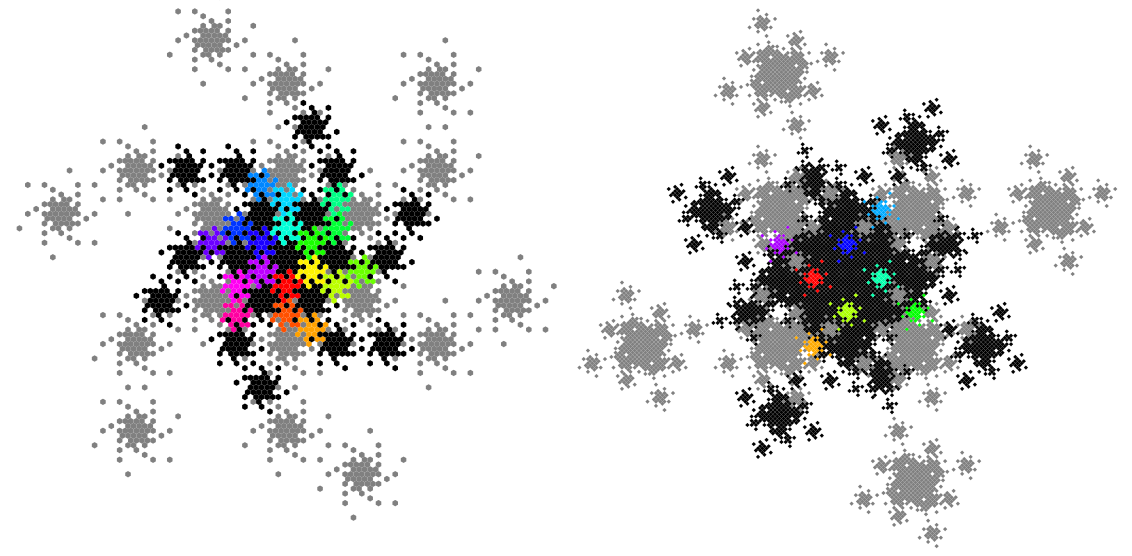
\includegraphics[width=15cm]{images/dessin.png}
\caption{3-NAF on the left, 4-NAF on the right - for different $\tau \in \mathbb{C}$}
    \end{figure}


					

\begin{itemize}	
	\item Binary Non Adjacent Form, 2-adic NAF form, 1-width 2-adic NAF form: \\
		Condition on the digits are relaxed allowing the
		coordinate $-1$ in addition to $0$ and $1$: 
		\begin{center}
			$\mathcal{D} =\{ -1,0,1\}$\\
		\end{center}
		\begin{center}
			\textbf{'NAF' meaningless   vs   ' 1-width 2-adic NAF' meaningful}\\
		'1-width' refers the maximum value in $\mathcal{D} $, \\
		'2-adic' refers to base's expansion, 2	
		\end{center}

	\begin{mythm}[Reitwiesner' 1960] 
		For a $a \in \mathbb{N} $, there exits a unique signed binary expansion noted, 
		$(a_i)_{0 \leq i \leq t-1 }$,
		 called the 1-width 2-adic NAF form of $a$
		such that:
		\begin{center}
		     $a =  \sum \limits_0^{t-1} a_1 \times 2^i$, with $a_i \in \mathcal{D} =\{ -1,0,1\}$ \\
		     $\forall i \in \llbracket 0,t-1 \rrbracket,   a_i \times a_{i+1} =0$
		\end{center}
        \begin{figure}[!h]
            \centering
        	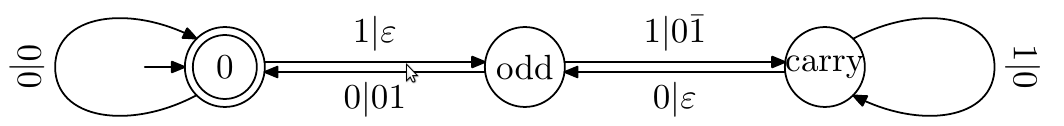
\includegraphics[width=15cm]{images/RtoL_unsignedbinary_to_2naf.png}
   		\end{figure}
	\end{mythm}


			\begin{center}
				\begin{tabular*}{10cm}{p{1.75cm}p{0.35cm}p{0.35cm}p{0.35cm}p{0.35cm}p{0.35cm}p{0.35cm}p{0.75cm}}		
     $ 23_{10} = \{$  &  0  &   1 &  0  &  1  &  1  &  1  &  $\}_2$\\	
     $ 23_{10} = \{$  &  0  &  1  &  1  &  0  &  0  & -1  &  $\}_2$\\
     $ 23_{10} = \{$  &  1  &  0  & -1  &  0  &  0  & -1  &  $\}_2$\\
				\end{tabular*}
			\end{center}

			Binary to binary 1-NAF definitions are not incompatible:
			\begin{center}
				\begin{tabularx}{10cm}
{p{1.5cm}p{0.35cm}p{0.35cm}p{0.35cm}p{0.35cm}p{0.35cm}p{0.35cm}p{0.75cm}}
$ 42_{10} = \{$  &  1  &   0 &  1  &  0  &  1  &  0  &  $\}_2$\\	
				\end{tabularx}
			\end{center}


    \begin{figure}[!h]
        \centering
        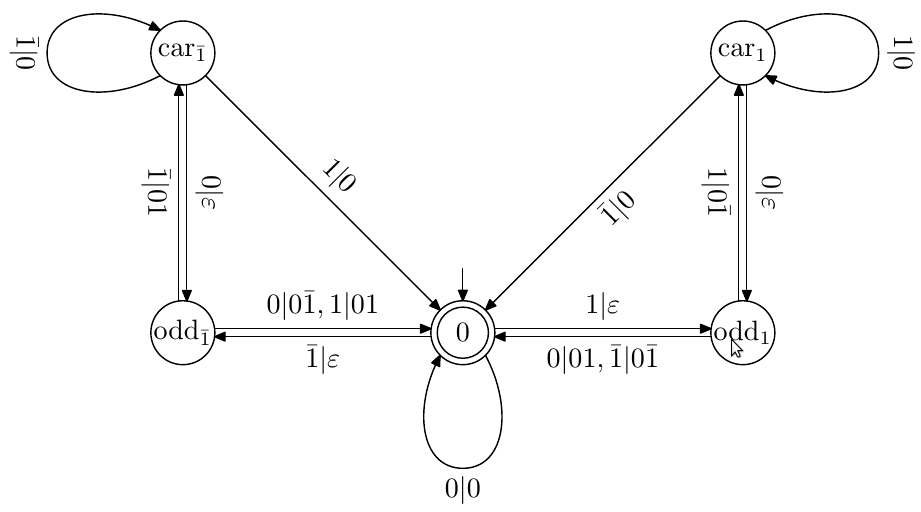
\includegraphics[width=15cm]{images/RtoL_allsignedbinary_to_2na0f.png}
		\caption{Visual proof for previous affirmation}
    \end{figure}

    \begin{mydef}{Optimality for a given digits space} :			
			An expansion of $a$  is said to be optimal, if it minimizes the weight
			among all the of $a$ with digits out of $\mathcal{D}$.\\
	\end{mydef}
		
	\begin{mythm}[Reitwiesner' 1960] 
			binary-NAF of integers is optimal among all expansion
			using the following digits $\mathcal{D} =\{ 0,\pm 1\}$.				
	\end{mythm}
			
		\underline{Theorems:} 
\begin{itemize}
\item 2-adic NAF representation have , at most, one digit longer than its a binary representation.
\item Each integer has a unique 2-adic NAF representation.
\end{itemize}

\textbf{1-width 2-adic NAF form: ECC vs RSA}
\begin{itemize}
\item[RSA case:] 'Square-and-Multiply' has to be changed to 'Square-and-Multiply-or-Divise'\\
and the value $x^{-1} \mod n$ shall be precomputed.\\ 
\item[ECC case:] 'Double-and-Add' algorithm should be changed to 'Double-and-Add-or-Substract' \\
and the value $-P $ should be precomputed.

But here is a trick : in many ECC implementation compute the opposite of a point 
is very easy: in this case: binary NAF applied to ECC saved a pre-computed value 
by comparison to RSA the same representation applied to RSA.
\end{itemize}





\newpage
	\item Extended Binary NAF or $k$-width 2-adic NAF, canonical representation\\
		extension of the 2-NAF: the base is still $\tau=2$,
		but the digit space is increased ...
			\begin{center}
$a =  \sum \limits_0^{t-1} a_I \times 2^i$,
with $a_i \in \mathcal{D} =\{ 0,\pm 1, \pm 3, .., \pm 2^{k-2}-1 \}$ \\
$\forall i \in \llbracket 0,t-1 \rrbracket,$
Among $k$ consecutive digits max one of them is non-zero\\
Each non zero digit is odd.
			\end{center}

%			width 	max digits 		formula
%2 			+/- 1  		2^(2-1)-1
%3 			+/- 3  		2^(3-1)-1
%4 			+/- 7  		2^(4-1)-1
%5 			+/- 15  	2^(5-1)-1

		\underline{Theorems:} 
\begin{itemize}
\item $k$-width 2-adic NAF representation, 
at most, one digit longer than its binary representation.
\item Each integer has a unique $k$-width 2-adic NAF.
\end{itemize}

		\underline{Theorem:} Avanzi, Muir \& Stinson' 2004\\
		With $\tau = 2$, $k \geq 2$, extended binary NAF of each integer 
		is optimal for $\mathcal{D} =\{ 0,\pm 1, \pm 3, .., \pm 2^{k-2} \}$.	
	



\end{itemize}						
		\underline{General converter}
			The following routine returns the $\omega$-width binary NAF of a binary 
			
			\begin{algorithm}[h]
				\KwIn{$n \in \mathbb{N}$}
				\KwOut{$n \in \mathbb{N}$}										 
				\If{ $n=0 \mod 2$  }{ \Return{$ n/2 $}	} 					 
				$r \leftarrow -2^{k-1}<r \leq 2^{k-1}$ 
				with $n = b \times 2^k + r$. \;					
				\Return{$n\leftarrow (n-r)/2^{\omega}$  }									
				\caption{function $f_\omega(n)$}
			\end{algorithm}	
			\begin{algorithm}[h]
				\KwIn{$n \in \mathbb{N}$}
				\KwOut{$n \in \mathbb{N}$}										 
				\If{ $n=0 \mod 2$  }{ \Return{$ 0 $} } 
				$r \leftarrow -2^{k-1}<r \leq 2^{k-1}$ with $n = b \times 2^k + r$. \;	
				$0^{k-1}r$			 				
				\caption{function $g_\omega(n)$}
			\end{algorithm}					
			\begin{algorithm}[h]
				\KwIn{$n \in \mathbb{N}$}
				\KwOut{a string of digits}	
				$\alpha \leftarrow$ ''												 
				\While{ $n \neq 0$ }{
				$\alpha \leftarrow g_{\omega}(n)\,||\,\alpha $\;
				$ n \leftarrow f_{\omega}(n)$ 
					} 
				\Return{$ \alpha $}												 				
				\caption{Binary to $\omega$NAF converter}
			\end{algorithm}	

	
\underline{examples}\\
$g(2)(n)$ will take the values: $     0, 01, 01, 01$\\
$f(2)(n)$ will take the values: $42, 21,  5,  1, 0$\\
then the 2NAF form of 42 is $0101010_2$ meaning $42_{10}= 2^5+2^3+2^1$.
		
$g(3)(n)$ will take the values: $ 0,  00-3, 003$\\
$f(3)(n)$ will take the values: $42,  5,    1, 0$\\
then the 3NAF form of 42 is $300-30_2$ meaning $42_{10}= 3 \times2^4 -3 \times 2^1$.		

$g(4)(n)$ will take the values: $ 0,  00-3, 003$\\
$f(4)(n)$ will take the values: $42, 21, 3, 0$	\\
then the 4NAF form of 42 is $300-30_2$ meaning $42_{10}= 3 \times2^4 -3 \times 2^1$.

$g(5)(n)$ will take the values: $ 0, 0000-11, 0002$\\
$f(5)(n)$ will take the values: $42, 21, 1, 0$\\
then the 5NAF form of 42 is $000010000-10_2$ meaning $42_{10}= \times2^7 -11 \times 2^1$..
%	3 0 0 -3 0  = 3 * 2^4 + 0 * 2^3 + 0 * 2^2 + 3 * 2^1 + 0 * 2^0 = 42.
%
%w = 3, then f3(13) = 2 and g3(13) = 00-3.

\newpage
\textbf{$k$-width 2-adic NAF form: ECC vs RSA} ... example with $k=3$
\begin{itemize}
\item[RSA case:] 'Square-and-Multiply' has to be changed to 'Square-and-Multiplyor-Divise'\\
and the values $\{ - 1, \pm 3 \} $ shall be precomputed.\\ 
\item[ECC case:] 'Double-and-Add' algorithm should be changed to
'Double-and-Add-or-Substract' \\
and only the value $3P $ should be precomputed, in the case of a curve 
giving cheap inversion.

	\item Real Non-Binary based NAF: Non-Binary NAF and Non-Binary $k$-NAF:\\
    Here simply the base $\tau$ is not two any more, but another prime.    

	\item Complex NAF and $k$-NAF form:\\
		This time is $\tau \in \mathbb{C}^\ast$ and is algebraic integer over
		$\mathbb{Z}$ of degree 2 
		\footnote{\textit{i.e} root of some $x^2-p \times x + q \in \mathbb{Z}$[x]}
		with $|\tau| > 1$ and $k \geq 2$
 
	\begin{mydef}
	 \textit{Zero \& local Voronoi Cells:}\\
		The Voronoi cell at origin is :
 		\begin{center}
 		$V :=\{ z \in \mathbb{C}: \forall y \in \mathbb{Z}^{\ast}[\tau],
 		\|z\|\leq \|z-y\| \} $
 		\end{center}
 		 		By definition the Voronoi Cell for the point $u \in \mathbb{Z}[\tau]$ 
 		corresponding to set $\mathbb{Z}[\tau]$ where $u$ is then called 
 		centre of $V_u$, or the lattice point corresponding to $V_u$, is such as:
 		\begin{center}
 		$V_u :=\{ z \in \mathbb{C}: \forall y \in \mathbb{Z}[\tau],
 		\|z-u\|\leq \|z-y\| \} $
 		\end{center}
	\end{mydef}

        \begin{figure}[!h]
          \centering
          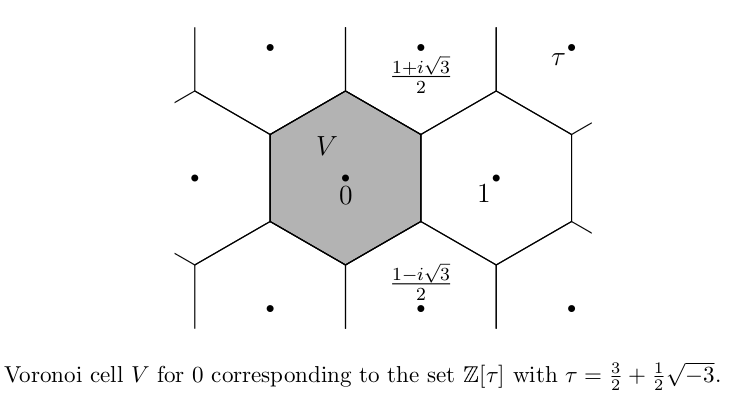
\includegraphics[width=15cm]{images/voronoi.png}
        \end{figure}
        Remark that the limit case given by equation of the definition
 		$ \|z\| = \|z-y\| $ share the plan in two via the bisection of 
 		segment $[zy]$ which fully make sense when $z$ is an extremal point.
        \newpage

        \raggedleft 
		... From now on $\mathcal{D}$ is assumed to be a 'Restricted Voronoi Cell' \\
		\raggedright		
	\begin{mydef} \textit{Restricted Voronoi Cell:}\\
        Previous definition was unclear about to which cell borders 
        -vertices + edges- belong to.
        Each edge is split in two equal part, defining three points of each of them,
        defining twice more points and portions of line than there was of vertices 
        and edges, then those elements are fairly shared (segment , points) 
        on each side of the origin.         
        This new cell is called 'Restrictive Voronoi Cell', and noted $\tilde{V}$
        \begin{figure}[!h]
          \centering
          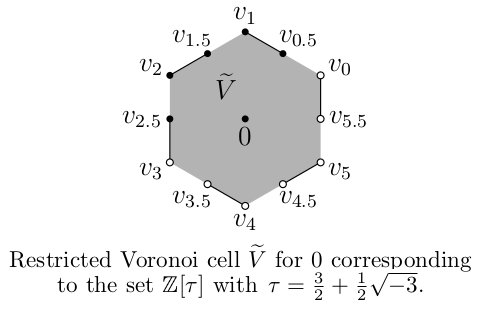
\includegraphics[width=10cm]{images/voronoi_restricted.png}
          \caption{     \textit{if $stuff \in V_u$ then its symmetrical don't}.}
        \end{figure}
    \end{mydef}
\raggedleft 

... From now on $\mathcal{D}$ is assumed to be a 'Reduced Residue Digit Set' \\
\raggedright
	\begin{mydef}{Reduced Residue Digit Set}\\
		For $\mathcal{N}(\tau^k) \leq 12$, we note 
		\begin{center}
		$R = \{x \in \mathcal{O}_\mathbb{K}$ such that $\tau \not\vert x \}$
		\end{center}
		The set $\mathcal{D} \subseteq \mathbb{Z}[\tau]$ is called 
		'reduced residue digit set modulo $\tau^k$', 
		if it consist of $0$ and exactly one representative for each 
		residue class of $R \mod \tau^k$ that is not divisible by $\tau$.
		
		More precisely:\\ 
		if a class contain a unit $u$ then: 
		$\mathcal{D} := \mathcal{D} \cup \{u\}$\\
		if a class do not contain a unit: 
		$\mathcal{D} := \mathcal{D} \cup \{u$ such that $ |u|\leq \mathcal{N}(\tau^k) \}$\\
	\end{mydef}
\vspace{5mm}


\textbf{Definition:} 
\textit{RDS $k$-Width $\tau$-adic Non Adjacent Form} 
or  
\textit{$k$-Width NADS:}
\\
Let's  $\mathbf{\eta}=(\eta_j)_{j} \subset \mathcal{D}^\mathbb{Z}$ .
The representation $ \eta $ is called $k$-Width $\tau$-adic Non Adjacent Form
if each factor $\eta_{j+k-1}...\eta_{j}$, \textit{i.e.} each block of length $k$
contains, at most, one non-zero digit.
\vspace{5mm}

\textbf{Theorem} 
\begin{center}
	Let's $k>2$, $\mathbb{K}=\mathbb{Q}[\tau]$ and  $\mathcal{D}$ 
	be a $k$-Width NADS and  \\
	we have $\forall x \in \mathcal{O}_\mathbb{K}, \; \exists ! $ 
	RDS $k$-Width $\tau$-adic NAF for $x$.
\end{center}

Remark: in certain cases the condition $k>2$ can be relaxed:

for $ \tau = \frac{3+\sqrt{-3}}{2}$, $k>1$\\
for $ \tau = \frac{1+\sqrt{-7}}{2}$, $k>1$\\
for $ \tau = \frac{1+\sqrt{-11}}{2}$, all $k$ \\

\newpage
\raggedleft 
... From now on element of $\mathcal{D}$ are assumed to be a
'Representatives of Minimal Norm' \\

\raggedright
	\begin{mydef}{Representative of Minimal Norm}\\
			Let $\tau$ be an algebraic integer, imaginary quadratic and let 
		$\eta \in \mathbb{Z}[\tau]$ be not divisible by $\tau$. \\
		Then if $\eta \in \tau^k \times \tilde{V}$ is called 
		'Representative of Minimal Norm'

        \begin{figure}[!h]
          \centering
          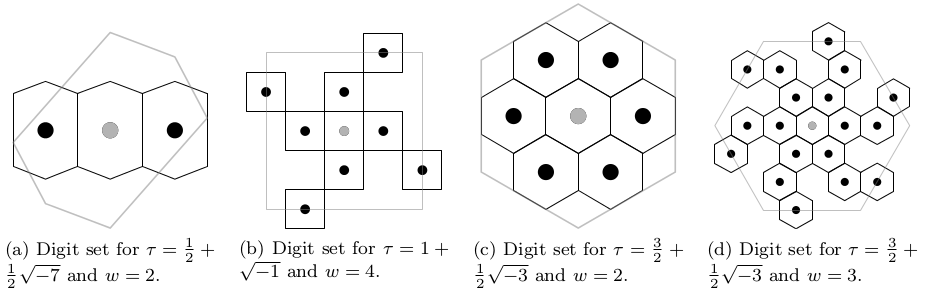
\includegraphics[width=18cm]{images/voronoi_save.png}
        \end{figure}
    \end{mydef}

\begin{itemize}
\item Minimal norm representatives digits set modulo  $\tau^k$ for several $\tau$ and $k$.
\item For each $\tau$, $V_\tau$ is drawn; the large cell is $\tau^k \times V$.
\item the situation c) verify the previous definition 
\end{itemize}
\vspace{3mm}

\raggedleft 
... From now on element of $\mathcal{D}$ are assumed to be a 'Minimal Norm Representative Digit Set' \\
\raggedright
		Definition - \textit{Minimal Norm Representative Digit Set:} \\
		Let $\tau$ be an algebraic integer, imaginary quadratic 
		and let $\mathcal{D}$ be reduced residue digit set modulo $\tau^k$
		consisting of representative of minimal norm if its residue class,
		then $\mathcal{D}$ is called 'Minimal Norm Representative Digit Set'.\\
\vspace{3mm}

.... And here it is:
\vspace{3mm}

		\textbf{Definition} \textit{$k$-Width $\tau$-adic Non Adjacent Form:} \\
Let's  $\mathbf{\eta}=(\eta_j)_{j} \in \mathcal{D}^\mathbb{Z}$ .
The representation $ \eta $ is called $k$-Width $\tau$-adic Non Adjacent Form

if each factor $\eta_{j+k-1}...\eta_{j}$, \textit{i.e.} each block of length $k$
contains, at most, one non-zero digit.\\
\vspace{3mm}

\begin{mythm} 
	For each lattice point  $x \in \mathbb{Z}[\tau]$ 
	and  $\mathcal{D}$ be a $k$-Width MNR\\
	we have $\forall x \in \mathbb{Z}[\tau], \; \exists ! $ 
	MNR $k$-Width $\tau$-adic NAF for $x	$.
\end{mythm}

\vspace{5mm}		
		\underline{Theorem:} Avanzi, Muir \& Stinson' 2004\\
		In the complex case with $\tau = 2$, $k \in \{2, 3\}$,
		the $\tau^k$-NAF  is optimal.

		\underline{Theorem:} Heuberger' 2010\\
		In the complex case with $k \in \{4,5,6\}$,
		the $\tau^k$-NAF is NOT optimal.


		\underline{Theorem:} Krenn' 2011\\
		In the following cases:
		$k \geq 4$, $\|p\| \geq 3$ or $k = 3  $, $\|p\| \geq 5$ 

		In the complex case with $k \in \{4,5,6\}$,
		the $\tau^k$-NAF is optimal.

	\end{itemize}
		\underline{Example:} binary to binary NAF conversion\\
			 An intuitive algorithm without pretending to any efficiency is
			'starting form LSB if two consecutive non zeros digit are meet
			change the smallest for -1 and propagate the change. 
			
			The process will always terminates with a valid NAF representation of $n$,
			process start and begin at position entirely determined	by ${n_2}$, 
			noting that the it is a fully reversible process.
			   			     
\underline{Important remark:}
Strictly speaking the difference between a Square \&  Multiply and a $2^3$-arry 
method is only a change in the representation from base 2 to base $2^3$, 
and using the same exponentiation algorithm.

		 
\newpage		
\subsubsection{Illustration of complex NAF:}



This section is dedicated to give an basically meaningful example 
of use of complex NAF, the given example is for primary field, then 


Let assume $ P $ is a point on the hereafter defined curve$ \mathbb{E} $,
and let $n$ and integer and $n P$ to be computed.

\begin{center}
$\mathbb{E}({\mathbb{F}_5}^m):  y^2 = x^3 -x  +2$ over $ {\mathbb{F}_5}^m $
\end{center}

How many point on the curves $\mathbb{E}({\mathbb{F}_5}^m)$? depending on $m$\\
How many point on the curves $\mathbb{E}({\mathbb{F}_5})$? let's see
		

%\noindent
%\begin{minipage}{\textwidth}[t][0.5 \textheight][t]

%\end{minipage}

	\begin{figure}[htbp]
		\begin{minipage}[c]{.70\linewidth}
			\begin{center}
				\begin{tabular}{|p{15mm}|p{15mm}|p{15mm}|p{15mm}|}
					\hline \rowcolor[rgb]{.8,.8,.8} 
					$x$ & $x^3 -x  +2$ & $y$ & $ y^2$\\
					\hline
					$ 0 $ & $ 2 $ & $ 0 $ & $ 0 $\\
					\hline
					$ 1 $ & $ 2 $ & $ 1 $ & $ \mathbf{1} $\\
					\hline
					$ 2 $ & $ 3 $ & $ 2 $ & $ 4 $\\
					\hline
					$ 3 $ & $ \mathbf{1} $ & $ 3 $ & $ 4 $\\
					\hline
					$ 4 $ & $ 2 $ & $ 4 $ & $ \mathbf{1} $\\
					\hline
				\end{tabular}						
			\end{center}		
		\end{minipage}
		\hfill
		\begin{minipage}[c]{.30\linewidth}	
			$\mathcal{O}$\\
			$(3, \pm 1)$\\
			$(3, \pm 4)$\\
		\end{minipage}
		\caption{$\mathbb{E}({\mathbb{F}_5}) = \{ \mathcal{O} ; (3, \pm 1) \}$}
	\end{figure}
Then we define the Frobenius isomorphism as usual:
\begin{center}
 $ \sigma=\left\{ 
 \begin{array}{ll}  
 \mathbb{E}  \longrightarrow \mathbb{E} \\
  (x,y) \mapsto (x^5,y^5)
 \end{array} \right.$
\end{center} 

Then according to REFERENCE, Frobenius morphism has for characteristic polynomial:
$\Phi^2 -a \times \Phi +q$ where $a = q+1 - \mathbb{E}({\mathbb{F}_q}) $ and here $q=5$
That is to say $\Phi^2 -3 \times \Phi + 5$

The previous decomposition lead us to use representation in $\mathbb{Q}[\sqrt{-11}]$

Avoid weakness on $\mathbb{E}({\mathbb{F}_5}^m)$, $m$ should not be stupidly chosen.

Then $\omega$-width $\tau$-adic NADS is prepared, with $\tau = \frac{1+\sqrt{-11}}{2}$,
According to the value of $\omega$, the digit space of $ \mathbb{D} $ is defined 
and $\omega$-width $\tau$-adic NADS conversion algorithm is defined.

\begin{enumerate}
\item Check that the considered representation exist
\item Convert $n$: compute $a+b \times \tau$ such that 
	$n \equiv a+b \times \tau \mod (\tau^m -1)$ 

	this trick has a name!\\
	since $(\tau^m -1) \times P =\mathcal{O}$, we have $n \times P = ( a+b \times \tau) P$

\item Convert $ a+b \times \tau$ to $\omega$-width $\tau$-adic NADS
\begin{center}
	$  a+b \times \tau  = \sum \limits_{i=0}^s c_i \tau^{k_i}$
\end{center}
\item for each $c \in \mathbb{D}$ pre-compute $Q_c = c \times  P$

\item Exponentiation is done trough a Horner scheme:\\
$(a+b  \tau) \times P  = 
\tau^{k_1}(\tau^{k_2-k_1} (... (\tau^{k_s-k_{s-1}}\times Q_{c_s} + Q_{c_{s-1}} )+ ... +)
+Q_{c_1})+Q_{c_0} $

\end{enumerate}
For binary fields, using normal basis, the cost of 'a Frobenius' is a shift



\subsection{Group representations}

\subsubsection{Chinese Theorem of Remainders:}
Elements of some finite fields $ \mathbb{Z}/{n \mathbb{Z}} $, 
where $n$ is a product of primes
\begin{itemize}
	\item Canonical representation in $ \mathbb{Z}/{n \mathbb{Z}} $,\\
	4 times slower tan CRT to achieve an RSA exponentiation.	
	
	\item Uses of Chinese theorem of remainders, 
	smaller number fastening the computations.
	Require a recombination step: Gauss, Garner, ...

	\noindent
	\textit{VS side channel cryptanalysis}\\
Because of the recombination step, that can be side channel analysed or even
perturbed, the CRT implementation bring also some potential weaknesses.
\end{itemize}

			\begin{algorithm}[h]
				\KwIn{$p, q, S_p, S_q, q^{-1}  \mod p, p^{-1}  \mod q$}
				\KwOut{$S = m^d \mod n$}	
				$S \leftarrow 
				S_p \times q \times (q^{-1} \mod p) +
				S_q \times p \times (p^{-1} \mod q) $\;	
				\Return{$ S $}												 				
				\caption{Gauss recombination}
			\end{algorithm}
			Remark: very natural but terribly slow as two modular inversions are required!
			\begin{algorithm}[h]
				\KwIn{$p, q, S_p, S_q, q^{-1}  \mod p$}
				\KwOut{$S = m^d \mod n$}	
				$t \leftarrow S_p-S_q$\;
				\If{ $t < 0$ }{ 
				$t \leftarrow t+p$\;
					} 
				$t^{'} \leftarrow t \times (q^{-1} \mod p)$	\;
				$S \leftarrow S_q + t^{'} \times q$\;	
				\Return{$ S $}												 				
				\caption{Unprotected Garner algorithm}
			\end{algorithm}
			
			\begin{algorithm}[h]
				\KwIn{$S_p, S_q, p, q, q^{-1}  \mod p$}
				\KwOut{$S = m^d \mod n$}	
				$t_0 \leftarrow S_p- S_q$\;
				$t_1 \leftarrow t_0 +p$\;
				\If{ $t_0 < 0$ }{ 
				$t \leftarrow t_1$\;
					}
				\If{ $t_0 > 0$ }{ 
				$t \leftarrow t_0$\;
					} 	 
				$t^{'} \leftarrow t \times (q^{-1} \mod p)$	\;
				$S \leftarrow S_q + t^{'} \times q$\;		
				\Return{$ S $}												 				
				\caption{Non conditional Garner algorithm}
			\end{algorithm}	
			
			\begin{algorithm}[h]
				\KwIn{$S_p, S_q, p, q, q^{-1}  \mod p$}
				\KwOut{$S = m^d \mod n$}	
				$t_0 \leftarrow S_p- S_q$\;
				$t_1 \leftarrow t_0 +p$\;
				\If{ $t_0 < 0$ }{ 
				$t \leftarrow t_1$\;
					}
				\If{ $t_0 > 0$ }{ 
				$t \leftarrow t_0$\;
					} 	
				$t^{'} \leftarrow t \times (q^{-1} \mod p)$	\;
				$S^{'} \leftarrow S_q + t^{'} \times (q+R)$\;
				$ S \leftarrow S^{'}  \mod  N$\;	
				\Return{$ S $}												 				
				\caption{Non conditional DPA-protected Garner algorithm}
			\end{algorithm}	







	    			\subsection{Multiplications}
\label{RSA_multipliction}

Beware that this is en attempt to separate each type operation -addition/soustration; multiplication; reduction; exponnetiation- whereas modern algorithm interleaves this operations ....

AIM: realize the following operation: compute $x \times y$ in the group $G$,
where $G$ is a general group. In some groups special algorithm can speed up 
multiplication algorithm, thanks to their rich algebraic structure and property:
this is the case of 'some' finite fields with Froebinius's isomorphism. 

\begin{itemize}
	\item  
		\begin{tabular*}{\linewidth}{ p{16cm} p{1.5cm}}
			Recursive method -\textit{Neanderthal}-  & $ -\infty $  \\
		\end{tabular*}	
			\noindent
			Multiply two numbers thanks to the definition of the multiplication 
			relying on the one of the addition.\\
			Complexity: $\bigO{n\times2^n}$.
	\item  	
		\begin{tabularx}{0.9\linewidth}{ p{16cm} p{1.5cm}}
			Knuth's schoolbook method -\textit{Neanderthal adult}-  & $0\%$ \\
		\end{tabularx}	
			\noindent
			This is the old method that is learnt in elementary school, also know as the Shift-And-Add method.
			Note that the famous Andrei Kolmogorov stated that this method was optimal! \\
			Complexity:  $\bigO{n^2}$.		

	\item 
		\begin{tabularx}{0.9\linewidth}{ p{16cm} p{1.5cm}}
			Gauss trick -\textit{1852}-  & $0\%$ 
		\end{tabularx}	

	\item  	\begin{tabularx}{\linewidth}{ p{16cm} p{1.5cm}}
			Quarter square method -\textit{Babylonian, 2000 BC}-  & $0\%$ \\ 
			\end{tabularx}	
			This method suppress multiplication for squarring, and is applcable since
			division by $4$ is allowed and $p$ is even.
			\noindent
			\begin{center}
			$			  \frac{(x+y)^2}{4} -  \frac{(x-y)^2}{4} =   \frac{1}{4}[(x^2+2xy+y^2)-(x^2-2xy+y^2)]= xy $
			\end{center}
			Or taking advantage of the parity:
			\begin{center}
			$			\lfloor  \frac{(x+y)^2}{4} \rfloor - \lfloor \frac{(x-y)^2}{4} \rfloor = xy $
			\end{center}

	\item  	\begin{tabularx}{\linewidth}{ p{16cm} p{1.5cm}}
			Revisited quarter square method -\textit{F.J.Taylor, 1981}-  & $0\%$ \\ 
			% https://tel.archives-ouvertes.fr/tel-00112121/document
			\end{tabularx}
			Quarter square method adapted to modular multiplication.\\	
			Method bounded to the same restrictions than the previous one.\\
			Taylor pre-computes: $\forall \hspace{1mm} 0 \leq x < p, MEM(x) = 4^{-1} x^{2}\mod p$\\
			The output is directly reduced $\mod p$, \textit{i.e.} no reduction and no mulitplication.\\
			But  $\#MEM  = p n$ bits.

	\item  	\begin{tabularx}{\linewidth}{ p{16cm} p{1.5cm}}
			Booth's algorithm-\textit{1951}-  & $20\%$ \\ 
			\end{tabularx}	
			\noindent
			This is a multiplication algorithm that multiplies two signed binary numbers in two's
			complement notation, used in the Infineon's ZDN algorithm. This multiplication algorithm is based 
			on a changed of the representation of numbers in two's complement notation.

	\item  	\begin{tabularx}{\linewidth}{ p{16cm} p{1.5cm}}
			Karatsuba's Method -\textit{1962}-  & $0\%$  
			\end{tabularx}	
			\noindent
			Divide and conquer applied to the classical multiplication algorithm: 
			numbers to multiply are divided in two equal parts, then using Gauss's 
			trick the result is obtained with only three multiplication (instead of four).\\
			Note that the week after Kolmogorof state that any algorithm would not be faster than $n^2$,
			one of his student, Anatolii Alexeevich Karatsuba, proved him he was wrong with this algorithm.\\
			Complexity:  $\bigO{3n^{log_2(3)}} \approx \bigO{3n^{1.55}}.$

			
	\item  	\begin{tabularx}{\linewidth}{ p{16cm} p{1.5cm}}
			Toom-Cook Algorithm -\textit{1963}-  & $- \infty$  
			\end{tabularx}	
			\noindent
			Generalise the previous method dividing each number to be multiplied in k 
			parts and it is typically used for intermediate-size multiplications, before using the 						asymptotically faster Schonhage Strassen algorithm. Not applicable to smart card.\\
			Complexity: $\bigO{n^{log(5)/log(3)}} \approx \bigO{n^{1.465}}  $

	\item  	\begin{tabularx}{\linewidth}{ p{16cm} p{1.5cm}}
			Schonhage-Strassen algorithm -\textit{1971}-  & $ -\infty $
			\end{tabularx}	
			\noindent
			Computation by isomorphism using FFT in rings with $2^n+1$, it is used in practice
			for numbers with more than 10,000 to 40,000 decimal digits. Not applicable to smart card.\\
			Complexity: $\bigO{nlog(n)log(log(n))}$. warning

	\item  	\begin{tabularx}{\linewidth}{ p{16cm} p{1.5cm}}
			Kochanski multiplication's -\textit{Kochanski 1985}-  & $20\%$ 
			\end{tabularx}	
			\noindent
			Kochanski multiplication is an algorithm that allows modular arithmetic (multiplication or 
			operations based on it, such as exponentiation) to be performed efficiently when the modulus 
			is large (typically several hundred bits). Widely used in constrained environment.
			
			
%	\item  	\begin{tabularx}{\linewidth}{ p{16cm} p{1.5cm}}
%			Reduced by feedback -\textit{Veilhaber 1987}-  & $00\%$ \\ 
%			\end{tabularx}	
%			\noindent
%			Algorithm discoverd (and forget) many times during the last 30 year

	\item  	\begin{tabularx}{\linewidth}{ p{16cm} p{1.5cm}}
			Furer's algorithm -\textit{2007}-  & $ -\infty $  
			\end{tabularx}	
			\noindent
			Improvement of the Schonhage-Strassen's algorithm.\\
			Complexity:  $\bigO{nlog(n)2^{ log^{*}(n)} }$ where $ log^{*} $ is the iterated logarithm.
			Not applicable to smart card.

	\item  	\begin{tabularx}{\linewidth}{ p{16cm} p{1.5cm}}
			Hardware multiplier -\textit{2000's}-  & $100\%$  
			\end{tabularx}	
			\noindent
			Especially dedicated multiplier, with a high efficiency.	
			According to a highly valuable source, namely wikipedia, hardware multiplier are,
			in general multiplying by $n$, using  the operation deduced from the following
			representation:
			\begin{itemize}
				\item Canonical binary representation
				\item Booth encoding
			\end{itemize}		
			But bit are not automatically scan 1 by 1.	
					

	\item  	\begin{tabularx}{\linewidth}{ p{16cm} p{1.5cm}}
			Masked Multiplication -\textit{2000's}-  & $100\%$  
			\end{tabularx}
			This is a generic counter-measure, to hide usage of multiplicands.
			\begin{center}	
			$p \times q  = (p-x) \times (q-x) + x \times (p+q) -x^2$
			\end{center}
			\noindent
			Simple method to blind operands

	\item 'As fast as you want'
	Nota, there exist a theoreme stating:\\
	Given $\epsilon>0$ there exists a multiplication algorithm such that the number 		
	of elementary operation $T(n)$ needed to multiply two m-bit digit numbers satisfies:
	\begin{center}
	$T(n) < c(\epsilon) \times n^{1+\epsilon} $
	\end{center}
	

\end{itemize}

	    			\subsection{Squarring} Maybe TBD
\label{RSA_squarring}
	    			\newpage
\subsection{Reduction}
\label{RSA_reduction}

Problem: $ T $ a number to reduce modulo $ N $, respectively $2n$ and $n$ bit long.\\
Aim: to deal efficiently with reduction modulo $N$, computation in $\mathbb{Z}/{N \mathbb{Z}}$.\\\\
\underline{References:}\\
\cite{crypto-1993-bosselaers}\\
\cite{arith-2007-hasenplaugh}\\
\cite{eprint-2014-zhengjun}

Duality between Multiplication and Modular Reduction: \cite{eprint-2005-fisher}
\begin{itemize}
	\item 
		\begin{tabularx}{\linewidth}{ p{14.5cm} p{3cm} }
		Euclidean method method -
		\textit{2000BC}- & $0\%$ 
	 	\end{tabularx}
	 		A complete Euclidean division is achieved:\\
	 		$ T = q N + r $ with $ 0 \leq r < N$\\\\
			\underline{Example:}\\
			Let's to be computed $x.y \mod N$  with $N = 119$, and $x = 63$, $y = 57$:\\
			$63.57 \mod 119 = 3591 \mod 119 = 119.30+21 \mod 119 = 21 \mod 119$\\
			But this requires a costly division which process is hidden...
		 		 
	\item
		\begin{tabularx}{\linewidth}{ p{14.5cm} p{3cm} }
		Knuth's "scholar" method - \textit{1969}- & $0\%$	  
		\end{tabularx}
		  	Improve the previous algorithm in the sense that only a 
		  	partial Euclidean division is performed.	  	
			
	\item 
		\begin{tabularx}{\linewidth}{ p{14.5cm} p{3cm} }
		Montgomery's reduction - \cite{ieeetc-2005-montgomery} - & $60\%$ \\
		\end{tabularx}
			Montgomery reduction algorithm is a pillar of modern modular calculus.
			It exists in many versions, with computation by bloc or globally
			with interleaved multiplication or not, and many more.\\

			Computation by isomorphism: computation are not performed in the original group 
			$\mathbb{Z}/{N \mathbb{Z}}$ but rather in another 
			representation of this ring.\\
			for $R$ co-prime with $N$, group isomorphism
			for $R$ co-prime with $N$ :
			$
			\phi\left\{
			    \begin{array}{c}
			     \mathbb{Z}/{N \mathbb{Z}} \longrightarrow {\mathbb{Z}/{N \mathbb{Z}}}^{'}  \\
			      \;\;\;\;x \longmapsto x.R
			    \end{array}
			\right.
			$
		    the operation corresponding
		    	    \footnote{
		    	Since $\phi(a).\phi(b) = a.b.R^2$, and  $\phi^{-1}(a.b.R^2)=a.b.R$
		    	}to the multiplication in $\mathbb{Z}/{n \mathbb{Z}}$
		    is $M_R (a,b)\mapsto a.b/R$
	
		    	   		  		   
			\begin{algorithm}
				\KwIn{
					$ T \in \mathbb{Z}/{R.N \mathbb{Z}}$ to reduce modulo $ N $ \\
					$ R, N \in \mathbb{Z}/{N \mathbb{Z}}$ such that $ pgcd(R,N) =1$\\
					$ N^{'} \in \mathbb{Z}/{R \mathbb{Z}}$ such that $R.R^{'}-N.N^{'}=1$
				}
				\KwOut{$ T.R^{-1} \mod  N $ }
				$m \leftarrow	 T.N^{'} \mod R$ \;
				$t \leftarrow	 (T+m.N).R^{-1}$ \;
				\If {$t \geq n$}{
					$ t \leftarrow T \mod  N $\;
					} 
				\Return{$ t $}\;
				\caption{Montgomery's reduction algorithm $redct$ function}
			\end{algorithm}				
			we have  an algorithm:
			\begin{itemize}
				\item achieving a division by $R$, that can be chosen under condition
				\item reducing its input modulo $N$
				\item without divisions by $N$, if $T \leq R.N$
			\end{itemize}

		\textbf{Proof:}
			It is clear that $ T = T + m.N \mod N $, with $R.R^{'}-N.N^{'}=1$ and 
			$ m = T.N^{'} \mod R$ we have: $  T + m.N = T- (T \mod R)$ then 
			$  T + m.N \leq RN + RN$ so that $ 0 \leq t \leq 2N $.

			Function  $redct$is used to multiply in Montgomery domain but also 
			to as 'transfer':\\
			Thanks to: $ redct(x.R^2) = x.R \mod N = \phi(x) $ and $redct(x) = x.R^{-1} \mod N = \phi^{-1}(x) $.

			In practice we can choose $R$ regarding the modulus pre-compute $R^2 \mod N$, $R^{-1} \mod N$\\
 		  
		\underline{Example:}
			Let's to be computed $x.y \mod N$  with $N = 119$, and $x = 63$, $y = 57$:\\
			Define isomorphism :
			choose a hardware compatible $R$ with the condition $R > N$,  $R =2^7 = 128$\\ 
			Precomputed values : $R^2 \mod N = 81$, $R^{-1} \mod  N = 53$\\
			Transfer data into Montgomery Domain: 
			\begin{center}
				$ \phi(x) = x.R \mod N  = redct(x.R^2) = redct(63.81) = 91 $\\
				$ \phi(y) = y.R \mod N  = redct(y.R^2) = redct(57.81) = 37$\\
			\end{center}
			Multiplication in Montgomery domain: 
			\begin{center}
				$ M_R(\phi(x),\phi(y)) = redct(91.37.53) \mod 119 = 70$
			\end{center}
			Return the result from the Montgomery domain: 
			\begin{center}
				$x.y \mod N = redct(70) = 21$	
			\end{center}
			
			All the division was by $R$, if $R$ is a power of two for the hardware this only a shift. 
			Secondly $R^{2}$ and $R^{-1}$ are precomputed values.	  
					   

	\item \begin{tabularx}{\linewidth}{ p{14.5cm} p{3cm} }
		Barrett's reduction -\textit{\cite{crypto-1986-barrett}} & Widely used 
		\end{tabularx}
		Involves one pre-computation: 
		$\mu = \lfloor \frac{2^{2n}}{N} \rfloor$.\\
		The reduction take the form:
		\begin{center}
			$R = T - \lfloor \lfloor \frac{T}{2^{n}} \rfloor \frac{\mu}{2^{n}} \rfloor N$\\
		\end{center}		

		Requires: two +1 n-bit multiplications and on subtraction.

		\underline{Example:}
			$x.y \mod N$  with $N = 119$, and $x = 63$, $y = 57$\\
			Precomputed values :
			$\mu  = \lfloor 2^{16}/119 \rfloor  = 550$\\
			
			The reduction take the form\\
			$R = 3591 - \lfloor \lfloor \frac{3591}{2^{8}} \rfloor \frac{550}{2^{8}} \rfloor 119$\\
			$R = 3591 - \lfloor 14 \times 2.148 \rfloor 119$\\
			$R = 3591 - 30.119$\\
			$R = 3591 - 3570$\\
			$R = 21 $ 


	\item \begin{tabularx}{\linewidth}{ p{14.5cm} p{3cm} }
		Iterative folding -\textit{\cite{arith-2007-hasenplaugh}} & $0\%$ 
		\end{tabularx}
		Iterates a divide and conquer approach to have smaller multiplication, in Barrett's algorithm. This involve more pre-computations: 
		$\forall i, 1 \leq i \leq F, M^{(i)} = 2^{(1+2^{-i})n}$ \\
		and for the final Barrett step :
		$ \mu = \lfloor \frac{2^{2n}}{M}  2^{2^{-F}n}\rfloor$\\

		The reduction take the form\\
		$N^{(0)} =N$\\
		$N^{(i)} =N^{(i-1)} \mod M^{(i)} + \lfloor \frac{N^{(i-1)}}{M^{(i)}}  \rfloor M^{(i)}\forall i, 1 \leq i \leq F$\\
		$	R = N^{(F)} - \lfloor \lfloor \frac{N^{(F)}}{2^{(1+2^{-F})n}} \rfloor \frac{\mu}{2^{2^{-F}n}} \rfloor M$\\

		Optimal for $F=2$

		\underline{Example:}
			Let's to be computed $x.y \mod N$  with $N = 119$, and $x = 63$, $y = 57$:\\
			Precomputed values : $N$ is 8 digits, we set $F=2$:\\
		$
		M^{(1)} = 2^{(1+2^{-1})8} = 2^{12} = 4096 \\
		M^{(2)} = 2^{(1+2^{-2})8} = 2^{10} = 1024$ \\
		And for the final Barrett step :\\
		$ \mu = \lfloor \frac{2^{16}}{119} 2^{2^{-2}8} \rfloor = \lfloor \frac{2^{16}}{119} 4 \rfloor = 2202$\\

		The reduction take the form\\
		$N^{(0)}= 3591$\\
		$N^{(1)}= 3591 \mod 2^{12} 	+ \lfloor \frac{3591}{2^{12}}  \rfloor M^{(1)}
				= 3591 \mod 2^{12} 				+ \lfloor \frac{3591}{2^{12}}  \rfloor 4096 = 3591$\\
		$N^{(2)}= N^{(1)} \mod 2^{(1+2^{-2})8} 	+ \lfloor \frac{3591}{2^{10}}  \rfloor M^{(2)}
				= 3591 \mod 2^{10} 				+ \lfloor \frac{3591}{2^{10}}  \rfloor 1024 = 519 + 3072 =3591 $\\		
		$	R   = N^{(2)} - \lfloor \lfloor \frac{N^{(2)}}{2^{(1+2^{-2})n}} \rfloor \frac{\mu}{2^{2^{-2}n}} \rfloor M$\\
		$	R   = 3591 - \lfloor \lfloor \frac{3591}{2^{10}} \rfloor \frac{\mu}{2^{2}} \rfloor 119$\\
		$	R   = 3591 - 3 550.5* 119$\\


			$\mu  = \lfloor 2^{16}/119 \rfloor  = 550$\\
			
			The reduction take the form\\
			$R = 3591 - \lfloor \lfloor \frac{3591}{2^{8}} \rfloor \frac{550}{2^{8}} \rfloor 119$\\
			$R = 3591 - \lfloor 14 \times 2.148 \rfloor 119$\\
			$R = 3591 - 30.119$\\
			$R = 3591 - 3570$\\
			$R = 21 $ 



	\item 
		\begin{tabularx}{\linewidth}{ p{14.5cm} p{3cm} }
		Sedlack's reduction -\textit{1987}- & $0\%$ 
		\end{tabularx}
		
	\item 
		\begin{tabularx}{\linewidth}{ p{14.5cm} p{3cm} }
		Quisquater reduction -\textit{1990}- & $0\%$  
		\end{tabularx}	
		Source: \cite{birthday-2012-joye}		  
		Patent protected
	\item 
		\begin{tabularx}{\linewidth}{ p{14.5cm} p{3cm}}
		ZDN algorithm -\textit{Infineon technologies 1990's}-  & $0\%$  
		\end{tabularx}
			
		\noindent	
		A far effective, hardware-compatible algorithm, ZDN based modular multiplication
		was developed by Infineon. ZDN based modular multiplication replaces the
		multiplication and reduction operations with a single operation, which the
		system can execute in a single clock-cycle. This algorithm implements a 
		look-ahead Booth (LABooth) multiplication with ZDN based 
		(Zwei Drittel N , 2/3N in German) modular reduction (LARed). 
		This algorithm further improves on register constraints because it ensures
		that the partial product remains at approximately 2/3N. With this algorithm
		the multiplication and modular reduction are calculated completely in parallel
		WTF!.
		\vspace*{3mm}

		VS side channel cryptanalysis:\\
		* immune against SvsM discrimination		  
\end{itemize} 

\textit{Barrett vs Montgomery}\\
Similarities:\\
    Both require pre-computing various constants for a given modulus $N$. Their input range is $[0,N^2)$. \\
    Their last las step lies in $[0,2n)$, with a final fix-up step to reach the output range of $[0,n)$.\\
    They perform 2 internal multiplications per reduction.\\
    Their reduction phases avoid division or remainder by non-powers-of-2.

Differences:\\
    Montgomery reduction requires expensive conversion into and out of 'Montgomery form', whereas Barrett reduction operates on regular numbers directly. \\
    Montgomery is based on modular congruences and exact division, whereas Barrett is based on approximating the real reciprocal with bounded precision. \\

Consumption: ''\\
    If the modulus is $n$ bits long, 
    Montgomery: two $n$-by-$n$ bit multiplications yielding $2n$ bits. 
    Barrett: one $2n$-by-$n$ bit multiplication yielding $3n$ bits, plus a $n$-by-$n$ bit multiplications yielding $2n$ bits, 

Usage:\\
    Montgomery reduction is suitable for modular exponentiation but not for working with various unrelated numbers where Barrett reduction is a good candidate for both,but more expensive.\\
	    			\newpage
\subsection{Exponentiations}
\label{RSA_exponnentiation}
%warning reference wtf! \\\\

AIM: realize the following operation $ y = x ^ n $. 

\subsubsection*{Warning !}
Note that of the following algorithms might be implemented indifferently
in left-to-right or for right-to-left, or also in atomic or non atomic
version, and so on and so on... A lot of combination are possible. Warning
\subsubsection{Convention and Names !}

The famous routine \textbf{"Square \& Multiply"} was named this way for a descriptive purpose: when we are using it we are effectively squaring and multiplying.

On the other hand it's mathematical name is \textbf{"dichotomic exponentiation"}
insisting on the fact that to achieve the exponentiation, is proceeded to recursive
calls to a sub-routine and that for each call there are two possibility 
multiplication.

The name \textbf{"binary method"} has been given with the same spirit.
Starting from now we adopt this kind of naming for every algorithm relative to
exponentiation. In this section will be viewed other algorithm scanning not
one bit but several bits of the exponent at each recursion. To have a clear
naming we extend the previous convention to this other class of algorithms
with the following convention:

\begin{center}
\textbf{2-ary method:} each recursion
$2^1$ possibilities and bit scanned $1$ by $1$. \\
\textbf{$ \mathbf{2^k}$-ary method:} each recursion
$2^k$ possibilities and bit scanned $k$ by $k$.
\end{center}
\vspace{3mm}
Some might object that could be said that a 3-arry method is scanning bits 3 by 3.\\
\underline{Example:} What about $ x ^ {27} $ without multiplying?\\
If you have an efficient algorithm to compute third power and
you build on it an exponentiation algo with at each recursion
a possible multiplication by $x^0$, $x^1$, $x^3$.
This algorithm works in a representation of 27 in base 3, and can't be named
with the other convention.
It's named trichotomic exponentiation, ternary method or cube and multiply.
\vspace{3mm}

\textbf{Known algorithms:}
\vspace{3mm}

	\begin{itemize}
	\item 	
		\begin{tabularx}{\linewidth}{ p{16cm} p{1.5cm}} 
		Recursive method -
		\textit{Neanderthal}-  & $ - \infty $ \\ 
		\end{tabularx}	
			\noindent
			This method is simply applying the definition of the exponentiation 
			as a set of exponentiation to obtained the desired result. 
	
			Enjoy: some academic paper from 1986 has been found considering that this algorithm 
			was competitive.

			This method will always return the worst of all exponentiation chains:  $\{1, \; ... ,\;n \}$ which length $l(n)$ is $n$.	To compute $x^n$, $n$ successives power of $x$ are computed !

			\vspace{5mm}
\end{itemize}


			
		 	
	\newpage
\subsubsection{Two Square \& Multiply algorithms and the factor method}

\begin{itemize}
\item  	\begin{tabularx}{\linewidth}{ p{16cm} p{1.5cm}}
		LtoR Square \& Multiply - 
		\textit{Chandah-sutra of Pingala, a classic Hindu, 400AC}-  & $0\%$ \\ 
		\end{tabularx}	
			\noindent
			Method designed following the observation that squaring can faster than multiplying.
			A square is done each time that is scanned another bit of the exponent.
			A multiplication is done conditionally depending on the value ofthe scanned bit.
						
			Since $n > 4$ this is computationally more efficient than naive exponentiation.
			This method uses the same addition chain that 'Multiply always' but the same one than the LtoR Binary method.\\	
			\begin{figure}[h]
				\begin{center}
				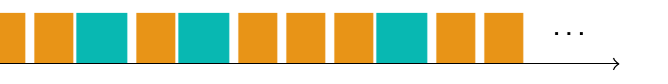
\includegraphics[scale=0.33]{images/SM.png}		
				\caption{$d_2 = 0 1 1 0 0 1 0 0 ... $}
				\end{center}
			\end{figure}	
			\begin{algorithm}[h]
				\KwIn{$x, {d =  d_{t-1} ... d_1 d_0}_{2}$}
				\KwOut{ $ y   =  x^d \mod n$ }
				 $y \leftarrow 1$ \;
				\For{$i  \gets t-1$ \textbf{to} $0$}
				{
				$y \leftarrow y^2 \mod n$\\				 
				\If{ $d_i= 1$  }{ 
					$y \leftarrow y \times x \mod n$	 
					} 
				}									 
				\Return{$ y $}\;
				\caption{LtoR dichotomic exponentiation}
			\end{algorithm}	

			\underline{Example :} LtoR Square \& Multiply: $n=23_{10}=10111_2$ the method starts 
			from the MSB.
			
			\begin{tabularx}{\linewidth}{ p{2cm} p{12cm} p{2cm}}
				$y=1$ & $ $\\
				$y:=y^2$ & $y:=y*x$	& $(y=x)$\\		
				$y:=y^2$ &       	& $(y=x^2)$\\
				$y:=y^2$ & $y:=y*x$ & $(y=x^{5})$\\
				$y:=y^2$ & $y:=y*x$ & $(y=x^{11})$\\
				$y:=y^2$ & $y:=y*x$ & $(y=x^{23})$
			\end{tabularx}	
			Powers of $x$ successively computed:	
			$x$ $x^2$ $x^4$ $x^5$ $x^{10}$ $x^{11}$ $x^{22}$ $x^{23}$, length 8\\
			
			\textit{Names}\\
			Algorithm also known as: 
			dichotomical exponentiation, Square \& Multiply, binary method. \\
			Do not mistaken this algorithm with its atomic version  as it is not 
			using a specialized routine for squaring it is also called sometime 
			'Multiply always'...		
							
			Note that the first non trivial step is always the same as we have 
			$d_{t_{min}-1} $, and will result in $y=x$ and therefore the it can be replaced for 
			an if.

			Which leads the number of operations to be performed to:
			\begin{center}
				$t_{min} + \omega_{\mathcal{H}}(d)-2$\\
				with $t_{min} =  \lfloor log_2(d) \rfloor$
			\end{center} 
			\newpage

\item  	\begin{tabularx}{\linewidth}{ p{16cm} p{1.5cm}} 
		RtoL Square \& Multiply-
		\textit{Al Kashi, 1427 AC}-  & $0\%$ \\
		\end{tabularx}	
			\noindent	

		Those two algorithms are exactly the same, those two versions are presented here.
		The fist version is scanning the bit form Right to Left, the second one is doing the 
		conversion on the fly starting from $d$.
		\textit{ $d_i= 1$ vs $d  \leftarrow \lfloor \frac{d}{2} \rfloor $ }.\\\\
		\begin{algorithm}[h]
			\KwIn{$x,n \in \mathbb{N}$, $x \leq n$}
			\KwOut{ $ y   =  x^d \mod n$ }
			$y \leftarrow 1$ \;		
			$local \leftarrow x$ \;	
			\While{$d  \neq 0$ }{			 
			    \If{ $d \mod 2 = 1$  }{ 
			    	$y \leftarrow y \times local \mod n$	\;
				} 
			$d  \leftarrow \lfloor \frac{d}{2} \rfloor $\;
			$local \leftarrow y^2 \mod n$	
			}									 
			\Return{$ y $}\;
			\caption{RtoL dichotomic exponentiation -On the fly version-}
		\end{algorithm}		
		\begin{algorithm}[h]
			\KwIn{$x,n \in \mathbb{N}$, $x \leq n$, ${d =  d_{t-1} d_1 d_0}_2$}
			\KwOut{$ y =  x^d \mod n$}
			$y \leftarrow 1$ \;		
			$local \leftarrow x$ \;	
			\For{$i \gets 0$ \textbf{to} $t-1$}{			 
			\If{ $d_i= 1$  }{ 	
				$y \leftarrow y \times local \mod n$	
				} 
			$local \leftarrow y^2 \mod n$	
			}									 
			\Return{$ y $}\;
			\caption{RtoL dichotomic exponentiation}
		\end{algorithm}				

		\underline{Example:} RtoL Binary method: $n=15_{10}=1111_2$\\			
			\begin{tabularx}{\linewidth}{ p{2cm}  p{12cm} p{4cm}}
				$y=1  $ & $l=x$		& $(y=1,l=x)$\\
				$y:=y*l$ & $l:=l^2$ 	& $(y=x,l=x^2)$\\
				$y:=y*l$ & $l:=l^2$ 	& $(y=x^3,l=x^4)$\\
				$y:=y*l$ & $l:=l^2$ 	& $(y=x^7,l=x^8)$\\
				$y:=y*l$ &          	& $(y=x^{15},l=x^{16})$
			\end{tabularx}	
			Powers of $x$ successively computed:	
			$x$ $x^2$ $x^3$ $x^4$ $x^7$ $x^{8}$ $x^{15}$, length 7: 6 operations\\
			This is the smallest value of $n$ for which the binary method is not optimal:\\
			The factor method with $x^{15} = (x^{3})^{5}$, lead to 5 operations\\\\
		\underline{Example:} RtoL Binary method: $n=23_{10}=10111_2$\\			
			\begin{tabularx}{\linewidth}{ p{2cm}  p{12cm} p{4cm}}
				$y=1  $ & $l=x$		& $(y=1,l=x)$\\
				$y:=y*l$ & $l:=l^2$ 	& $(y=x,l=x^2)$\\
				$y:=y*l$ & $l:=l^2$ 	& $(y=x^3,l=x^4)$\\
				$y:=y*l$ & $l:=l^2$ 	& $(y=x^7,l=x^8)$\\
				         & $l:=l^2$  	& $(y=x^7,l=x^{16})$\\
				$y:=y*l$ &          	& $(y=x^{23},l=x^{16})$
			\end{tabularx}	
			Powers of $x$ successively computed:	
			$x$ $x^2$ $x^3$ $x^4$ $x^7$ $x^{8}$ $x^{16}$ $x^{23}$, length 8: 7 operations\\	

		Note that those algorithms are provided in a pedagogical way, in a real life implementation two multiplication can be skipped: the $d_i= 0$ step $y \leftarrow 1 \times x \mod n$ can be exchanged for a if. The last square is also useless and can be prevented.\\\\
		Which leads the number of operations to be performed to:
		\begin{center}
			$t_{min} + \omega_{\mathcal{H}}(d)-2$\\
			with $t_{min} =  \lfloor log_2(d) \rfloor$
		\end{center} 

\item  \begin{tabularx}{\linewidth}{ p{16cm} p{1.5cm}}
			Square \& Multiply Always  & $0\%$ \\ 
		\end{tabularx}	
		\label{Square_Multiply_Always}
		\noindent
		This a counter-measure, to prevent multiply vs non multiply discrimination.\\
		The SPA vulnerability of S$\&$M algorithms come from a possible square versus 
		multiply discrimination, coming from the algorithmic implementation of those routines.

			Solutions:
		\begin{itemize}
			\item \textit{'Mutliply Always' i.e. Naive 'Square \& Multiply'} \\
			replace squarings by multiplications, but slower still a condition remains ...
			\item \textit{'Square \& Multiply Always'} \\
			Whatever the need 'always multiply': if no multiplication is requirred place a bogus multiplication
			\begin{figure}[h]
				\begin{center}
	        	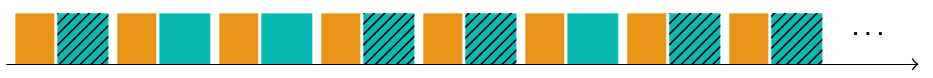
\includegraphics[scale=0.33]{images/SMA.png}
				\caption{LtoR Square \& Multiply Always illustration}
				\end{center}
			\end{figure}
			\item \textit{'Joye's Multiply Always' i.e. Atomic 'Square \& Multiply'} \\
			replace the squaring algorithm by a multiplying one: fully atomic algorithm.
		\end{itemize}

\item 	\begin{tabularx}{\linewidth}{ p{16cm} p{1.5cm}} 
		Square \& Multiply on the fly reduction-
		\textit{G.R.Blakley, 1983 AC}-  & $0\%$ \\
		\end{tabularx}	

\item 	Nota on Square \textit{vs} Multiply operands:

		When applying Square \& Multiply algorithm, additionally to the fact that
		the dedicated routines are different, there is structural difference between the two 
		fundamental operation:

		\begin{itemize}
			\item \textit{Square operations} possesses a variable operand, likely to change at each execution.
			\item \textit{Multiply operations} possesses a static operand, the $x$ to elevate to a certain power.\\
		\end{itemize}

\item 	\begin{tabularx}{\linewidth}{ p{16cm} p{1.5cm}} 
		Factor Method
		\textit{D.E.Knuth, 1908 AC}-  & $0\%$ \\
		\end{tabularx}	
		This method is recursive and is neither better or worst than the binary method.

		if $d$ is prime, compute $x \times x^{d-1}$\\
		if not and $d>3$, compute $ x^d = x^p \times x^{d'}$ with $p$ prime.

		The Factor Method is better than the binary method \textit{in average}.

		\underline{Example:} factor method: $n=15_{10}$\\			
			$x^{15} = (x^{3})^{5}$ and $x^{3} = x \times x^{2}$\\
			$x^{15} = x^{3} \times (x^{3})^{4}$\\
			$x^{15} = x^{3} \times ((x^{3})^{2})^2$\\
			Powers of $x$ successively computed:
			$x$ $x^2$ $x^3$ $x^6$ $x^{12}$ $x^{15}$, length 6: 5 operations\\
			This example is the first where the factor method is better than the binary method.

			But the factor method is not always better ...

		\underline{Example:} factor method: $n=33_{10} = 100001_2$\\			
			$x^{33} = (x^{3})^{11}$ and $x^{3} = x \times x^{2}$\\
			$x^{33} = x^{3} \times (x^{3})^{10}$\\
			$x^{33} = x^{3} \times ((x^{3})^{2})^5$\\	
			$x^{33} = x^{3} \times (x^{6})^5$\\
			$x^{33} = x^{3} \times x^{6} \times ((x^{6})^{2})^2$\\
			Powers of $x$ successively computed:
			$x$ $x^2$ $x^3$ $x^6$ $x^{12}$ $x^{24}$ $x^{30}$ $x^{33}$, length 8: 7 operations\\
			Whereas binary method requires $6 + 2 - 2=6$ operations...	

\end{itemize}


	
	\newpage
\subsubsection{Atomic Square \& Multiply}
\begin{itemize}
\item  	
		\begin{tabularx}{\linewidth}{ p{16cm} p{1.5cm}}
		Atomic Square \& Multiply - \lokiquote{ieeetc-2004-joye}
		\textit{Joye 2003}-  & $0\%$ 
		\end{tabularx}	
			\noindent

			\vspace{2mm}
			\textit{Generic counter measure} principle, based on the concept of 
			'side channel indistinguishability', applicable 
			to virtually all algorithms to protect them for SPA. 			
		
			Here is presented the version to protect the Square \& Multiply 
			algorithm against the SPA. Carefully note that $k$ is simply a boolean.			
			
			\begin{algorithm}[h]
				\KwIn{$x,n \in \mathbb{N}$, $x \leq n$, ${d =  d_{t-1} d_1 d_0}_2$}
				\KwOut{ $ y   =  x^d \mod n$ }
				$R_0 \leftarrow	 T.N^{'} \mod R$ 
				$R_1 \leftarrow	 T.N^{'} \mod R$ \;	
				$i \leftarrow t-1$
				$k \leftarrow 0$	\;	
				\While{$ i \geq 0$ }
				{			 
					 $R_0 \leftarrow R_0 \times R_k $ \;
					 $k \leftarrow k \oplus d_i $  \;
					 $i \leftarrow i - \textlnot k $  	
				}									 
				\Return{$ y $}\;
				\caption{Atomic Square \& Multiply - LtoR version}
			\end{algorithm}					
			\vspace{5mm}
									
   		\underline{Example:} 
   			LtoR version - Atomic Square \& Multiply:   			
   			$n=23_{10}=10111_2$\\
			\begin{tabularx}{\linewidth}{ p{2cm} p{11cm} p{3cm}}
				$R_0=1$ & $R_1=x$        	& $(k=0\;\;i=4)$\\
				$R_0=1$ & 		     	    & $(k=1\;\;i=4)$\\
				$R_0=x$ & 		     	    & $(k=0\;\;i=3)$\\
				$R_0=x^2$ & 		     	& $(k=0\;\;i=2)$\\
				$R_0=x^4$ & 		     	& $(k=1\;\;i=2)$\\
				$R_0=x^5$ & 		     	& $(k=0\;\;i=1)$\\
				$R_0=x^{10}$ & 		     	& $(k=1\;\;i=1)$\\
				$R_0=x^{11}$ & 		     	& $(k=0\;\;i=0)$\\
				$R_0=x^{22}$ & 		     	& $(k=1\;\;i=0)$\\
				$R_0=x^{23}$ & 		     	& $(k=0\;\;i=-1)$
			\end{tabularx}	
			
			\textbf{Remark that the same power of $x$ than in Square \& Multiply - LtoR version}
			\begin{center}
			$x$ $x^2$ $x^4$ $x^5$ $x^{10}$ $x^{11}$ $x^{22}$ $x^{23}$
			\end{center}


			So this algorithm is: using the same addition chain that Square \& Multiply to get 
			the final result as a LtoR S\&M, but in much more side-channel resistant way: 
			\begin{itemize}
				\item no condition: it is doing exactly the same thing at each recursion
				\item no squaring vs multiplication discrimination can be achieve from an 
				algorithmic point of view. 			
			\end{itemize}
            The price is no special routine is used to square, automatically slowing down the whole process 
            		
				
		\textit{Disambiguation}\\
			Because of the absence of squaring it is then frequently called
			'multiply always'  algorithm, please notice that is is ambiguous indeed, 
			see page \pageref{Square_Multiply_Always}.

		\textit{Conventional Names}\\
			"Joye's multiply always, LtoR version",  
			"Atomic Square \& Multiply, LtoR version"

		\textbf{Known Vulnerability}\\
		It have to be understood that this implementation is, by definition, absolutely 
		invulnerable to squaring vs multiplication discrimination 	
		\textbf{from an algorithmic point of view}.

		But it does not mean that it is invulnerable to squaring vs multiplication discrimination.
Indeed squaring vs multiplication discrimination can be achieved focusing on the hamming weight.

			
\end{itemize}							
	\newpage
\subsubsection{Scanning digits in base $2^k$}
\begin{itemize}
\item  	
		\begin{tabularx}{\linewidth}{ p{16cm} p{1.5cm}}
		Window Method: the LtoR $2^k$ary method: -
		\textit{Brauer 1939}-  & $0\%$  
		\end{tabularx}	
			\noindent
				Generalisation of the previous method, the bits of the exponent, in base 2, 
				are scanned $k$ by $k$, this method requires pre-computed values.
				Principle: $k$ squares are done each time scanning $k$ other bits of the exponent
				A multiplication by one of the $2^{k}-3$ pre-computed value is done 
				depending on the scanned group of bits..

				Only the precompuation of the $x^{d_j}$ such that $d_j$ appears in the representation of $d$ is needed.
				
			\begin{figure}[h]
			\begin{center}
	       		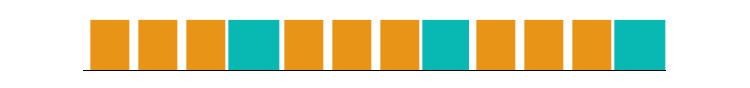
\includegraphics[scale=0.33]{images/2k.png}
				\caption{LtoR $2^k$ary method illustration, with $k=3$}
			\end{center}
			\end{figure}
			\begin{algorithm}[h]
				\KwIn{$x,n \in \mathbb{N}$, $x \leq n$, ${d =  d_{t-1} d_1 d_0}_2$}
				$x_0 \leftarrow 1$	\; 				
				\For{$ i = 0 \to 2^{k}-1$ }
				{						     
					 $x_i \leftarrow x_{i-1} \times x$ \;
				}
				$y \leftarrow 1$	\;
				\For{$ i = t-1 \to 0$ }
				{			 
					 $y = x^{2^k}$ \;
					 \If{$d_i > 0$}{
					 $y = y \times x_i$\;
					 } 	
				}									 
				\Return{$ y $}\;
				\caption{LtoR $2^k$-ary method}
			\end{algorithm}			

			\underline{Example 1:} LtoR $2^k$-ary method\\
			Let's assume that $m=8$ \textit{i.e.} $k=3$ with $n=326_{10}=101\;000\;110_2$ 
			the method start scanning the bits from their MSB but three by three.
			The precomputed values are:   $x^2$, ..., $x^7$\\
			\begin{tabularx}{\linewidth}{ p{2cm} p{2cm} p{2cm} p{8cm} p{2cm}}
				$y:= 1$ & & & &\\
				$y := y ^2$ & $y := y ^2$ & $y := y ^2$ & $y := y  \times  x^5$ & $(y=x^5)$ \\
				$y := y ^2$ & $y := y ^2$ & $y := y ^2$ & $y := y  \times  x^0$ & $(y=x^{40})$\\
				$y := y ^2$ & $y := y ^2$ & $y := y ^2$ & $y := y  \times  x^6$ & $(y=x^{326})$
			\end{tabularx}
			\vspace{3mm}
			
		\underline{Example 2:} LtoR $2^k$-ary method \\	
			Let's assume that:
			$n=11651101_{10}=101\;\;100\;\;011\;\;100\;\;100\;\;000\;\;011\;\;101_{2}$\\
			\begin{tabularx}{\linewidth}{ p{2cm} p{2cm} p{2cm}  p{8cm} p{4cm}}
				$y:= 1$	 &   		&          & $y:=y \times x^5$ & $(y=x^{5})$ \\
				$y:=y^2$ & $y:=y^2$ & $y:=y^2$ & $y:=y \times x^4$ & $(y=x^{44})$\\
				$y:=y^2$ & $y:=y^2$ & $y:=y^2$ & $y:=y \times x^3$ & $(y=x^{355})$ \\               
				$y:=y^2$ & $y:=y^2$ & $y:=y^2$ & $y:=y \times x^4$ & $(y=x^{2\,844})$\\
				$y:=y^2$ & $y:=y^2$ & $y:=y^2$ & $y:=y \times x^4$ & $(y=x^{22\,756})$\\       
				$y:=y^2$ & $y:=y^2$ & $y:=y^2$ & 				   & $(y=x^{182\,048})$\\
				$y:=y^2$ & $y:=y^2$ & $y:=y^2$ & $y:=y \times x^3$ & $(y=x^{1\,456\,387})$\\                 
				$y:=y^2$ & $y:=y^2$ & $y:=y^2$ & $y:=y \times x^5$ & $(y=x^{11\,651\,101})$\\		
			\end{tabularx}
			To get this result a certain decomposition of $n$ 
			was used which lead to 21 squarings and 7 multiplications.
			
			\underline{Name \& convention}							
				The $2^k$ary method may also be called $k$-bits Window method, 
				insisting on the number of bit scanned at each recursion...
			\newpage
	\item  	
		\begin{tabularx}{\linewidth}{ p{16cm} p{1.5cm}}
		Window Method: LtoR Optimized $2^k$-ary exponentiation: -  & $0\%$
		\end{tabularx}	
			\noindent
			Optimization of the previous method, only even power of $x$ are stored only.\\
			Require $ 2^{k-1}-1 $ precomputed values overall.
			\vspace{3mm}
			\begin{algorithm}[h]
				\KwIn{$x$, ${d =  d_{t-1} d_1 d_0}_{2^k}$}
				$x_0 \leftarrow 1$	\; 
				$x_1 \leftarrow x$	 \; 
				$x_2 \leftarrow x^2$  \; 				
				\For{$ i = 1 \to 2^{k-1}-1$ }
				{						     
					 $x_{2i+1} \leftarrow x_{2i-1} \times x_2$ \;
				}
				$y \leftarrow 1$ \;
				\For{$ i = t-1 \to 0$ }
				{			 
					 $y = x^{2^k}$ \;
					 \textbf{define:} $d_i = 2^{h_i} \times u_i $ 
					 where $u_i$ is odd and $ h_i $ maximal	\;		
					$y = {( y^{2^{k-h_i}} \times x_{u_i} )^2}^{h_i} $
				}									 
				\Return{$ y $}\;
				\caption{Optimized LtoR $2^k$-ary method}
			\end{algorithm}			
			
		\underline{Example:} LtoR Optimized $2^k$-ary exponentiation\\
			$n=326_{10}=101\;000\;110_2$ and $k=3$ \textit{i.e.} $m=8$ 
			the method starts scanning the bits from their MSB but three by three.
			The precomputed values are:   $x^3$, $x^5$, $x^7$.\\
			\begin{tabularx}{\linewidth}{ p{2cm} p{2cm} p{2cm} p{8cm} p{2cm}}
				$y:= 1$ & & & &\\
				$y := y ^2$ & $y := y ^2$ & $y := y ^2$ 			& 
				$y := y  \times  x^5$   &	$(y=x^5)$ \\
				$y := y ^2$ & $y := y ^2$ & $y := y ^2$ 			&
				$y := y  \times  x^0$ & $(y=x^{40})$\\
				$y := y ^2$ & $y := y ^2$ & $y := y  \times  x^3 $	& 
				$y := y  \times  x^2$ & $(y=x^{326})$
			\end{tabularx}
			
			Practical remark:
			\begin{center}
			On a SPA point of view it is crucial to know whether or not the 
			implementation is saving pre-computation !
			\end{center}						
			\begin{itemize}
				\item if precomputed value are optimized:
				the goal become to discriminate elevation to the $8^{th}$ power 
				from multiplication by $(x^i)_{ 2 \leq i \leq7 }$ and in this case 
				we will always have sequence of elevation to the $8^{th}$ power then 
				a multiplication (or not). But the pattern of the curve should match 
				exactly the key.
				
				\item in this case we will not always have sequence of elevation 
				to the $8^{th}$ power then a multiplication (or not). Compare the last
				 line of the previous example and the same line with the 8-arry method.
			\end{itemize}

\newpage
\item  	
		\begin{tabularx}{\linewidth}{ p{16cm} p{1.5cm}}
		Window Method: RtoL $2^k$ary method:   & $0\%$  
		\end{tabularx}	
			\noindent

			\begin{algorithm}[h]
				\KwIn{$x,n \in \mathbb{N}$, $x \leq n$, ${d =  d_{t-1} d_1 d_0}_2$}
				$x_0 \leftarrow 1$	\; 				
				\For{$ j = 1 \to 2^{k}-1$ }
				{						     
					 $R_j \leftarrow 1$ \;
				}
				$y \leftarrow x$	\;
				\While{$ m \leq n $}
				{			 
					 $d \leftarrow n \mod m $\;
					 \If{$d \neq 0$}{
					 $R[d] \leftarrow R[d]  \times y$\;
					 } 	
					 $y \leftarrow y^m$\;
					 $n \leftarrow \lfloor n/m \rfloor $\;			
				}
				$R[n] \leftarrow R[n] \times y$\;
				$ y \leftarrow R[m-1]$\;
				\For{$ j = m-2 \to 1$ }
				{						     
					$ R[j] \leftarrow R[j] \times R[j+1]$\;
				    $ y \leftarrow y \times R[j]$\;
				}					 
				\Return{$ y $}\;
				\caption{RtoL $2^k$-ary method}
			\end{algorithm}	

			\underline{Example :} RtoL $2^k$-ary method, $m=8$ \textit{i.e.} $k=3$ with $n=326_{10}$
			
			Initialization phase:\\
			$R = \{1,1,1,1,1,1,1\}$, $y:= x$, $m=8$, $n=326$

			While loop:\\
			$d = 326 \mod 8 = 6$, $R = \{1,1,1,1,1,x,1\}$, $y:= x^8$,  $n=40$\\
			$d =  40 \mod 8 = 0$, $R = \{1,1,1,1,1,x,1\}$, $y:= x^{64}$, $n= 5$

			End while:\\
			$R = \{1,1,1,1,x^{64},x,1,1\}$, $y:= 1$

			Recomposition phase:\\
			$j=6, R = \{1,		1,		1,		1,			x^{64},	x,	1\}$, $y:= x$\\
			$j=5, R = \{1,		1,		1,		1,			x^{65},	x,	1\}$, $y:= x^{66}$\\
			$j=4, R = \{1,		1,		1,		x^{65},		x^{65},	x,	1\}$, $y:= x^{131}$\\
			$j=3, R = \{1,		1,		x^{65},	x^{65},		x^{65},	x,	1\}$, $y:= x^{196}$\\
			$j=2, R = \{1,		x^{65},	x^{65},	x^{65},		x^{65},	x,	1\}$, $y:= x^{261}$\\
			$j=1, R = \{x^{65},	x^{65},	x^{65},	x^{65},		x^{65},	x,	1\}$, $y:= x^{326}$\\


		\textit{Variants:}\\			
			 right to left version, optimized version 
\end{itemize}		 								
	\newpage
\subsubsection{Sliding window algorithms}
\begin{itemize}
\item  	
		\begin{tabularx}{\linewidth}{ p{16cm} p{1.5cm} }
		LtoR static $2^k$ sliding window method:  & $0\%$ 
		\end{tabularx}	
			\noindent
			Adapt the previous method in minimizing the size of the window when possible.
			First of all maximum length for the window has to be defined, then then bit are scan 
			adapting the window size to isolate the zeros.
			
		\underline{Complexity}:\\
			The algorithm requires   $\omega - 1 + n$ squares 
			and, at most, $2^{\omega-1} - 1 +  \frac{n}{\omega}$  multiplications.
			\vspace{3mm}
		
\begin{algorithm}[h]
	\KwIn{$x,n \in \mathbb{N}$, $x \leq n$, ${d =  d_{t-1} d_1 d_0}_2$, $k$}
	\KwOut{ $ y   =  x^d \mod n$ }
	$x_1 \leftarrow x$	\; 
	$x_2 \leftarrow x^2$	\;		
	\For{ $ i = 0 \to 2^{k}$ }
	{						     
		$x_i = x_{2i -1} \times x_2$ \;
	}
	$y \leftarrow 1$	\;
	$i \leftarrow t-1 $ \;
	\While{$ i \geq 0 $}
	{			 
        \If{$d_i = 0$}{
	   		$ y \leftarrow y^2 $\;
			$ i \leftarrow i-1 $\;
		} \Else {
            $ s \leftarrow max(i-w+1,0)$ \;
			\While{$d_s=0$}{$s \leftarrow s+1 $}
			$ u \leftarrow \{d_i...d_s\}_2$\;
            $ y \leftarrow y^{2^{i-s+1}} \times x_{u} $\;
            $ i \leftarrow i-s+1 $\;
		}
	}				 
	\Return{$ y $}\;
	\caption{LtoR static $\omega$-sliding window method}
\end{algorithm}

		\underline{Example 1:} LtoR static $\omega$-sliding window method \\
			Let's assume that 
			$n=11651101_{10}=1011\;\;000\;\;111\;\;00\;1\;\;\;000000\;\;111\;\;0\;\;1_2$ and $\omega=4$\\
			\begin{tabularx}{\linewidth}{ p{2cm} p{2cm} p{2cm} p{2cm} p{2cm} p{2cm} p{2cm}}
				$y:= 1$   & 		 &          &		   &          &			 & $y:=y \times x^{11}$\\
				$y:= y^2$ & $y:=y^2$ & $y:=y^2$ & 		   &          &			 & \\
				$y:= y^2$ & $y:=y^2$ & $y:=y^2$ &    	   &	      &			 & $y:=y \times x^7$\\            
				$y:= y^2$ & $y:=y^2$ &          &          &          &			 & \\
				$y:= y^2$ &          &     		&	       &          &			 & $y:=y \times x$\\       
				$y:= y^2$ & $y:=y^2$ & $y:=y^2$ & $y:=y^2$ & $y:=y^2$ &	$y:=y^2$ & \\
				$y:= y^2$ & $y:=y^2$ & $y:=y^2$ &          &          &			 & $y:=y \times x^7$\\
				$y:= y^2$ &  		 &          &          &          &			 & \\
				$y:= y^2$ &  		 &          &          &          &			 & $y:=y \times x$	\\			
			\end{tabularx}


			$n=11651101_{10}=1011\;\;000\;\;111\;\;00\;1\;\;\;00000\;\;0111\;\;01_2$ and $\omega=4$\\
			\begin{tabularx}{\linewidth}{ p{2cm} p{2cm} p{2cm} p{2cm} p{2cm} p{2cm}}
				$y:= 1$   & 		 &          &		   &          & $y:=y \times x^{11}$\\
				$y:= y^2$ & $y:=y^2$ & $y:=y^2$ & $y:=y^2$ &          & \\
				$y:= y^2$ & $y:=y^2$ & $y:=y^2$ &    	   &	      & $y:=y \times x^7$\\               
				$y:= y^2$ & $y:=y^2$ & $y:=y^2$ &          &          & \\
				$y:= y^2$ & $y:=y^2$ &     		&	       &          & $y:=y \times x$\\       
				$y:= y^2$ &			 &			&          &          & \\
				$y:= y^2$ & $y:=y^2$ & $y:=y^2$ & $y:=y^2$ & $y:=y^2$ & $y:=y \times x^7$\\           
				$y:= y^2$ & $y:=y^2$ & $y:=y^2$ & $y:=y^2$ &          & $y:=y \times x$	\\		
			\end{tabularx}	
			\newpage
\item  	
		\begin{tabularx}{\linewidth}{ p{16cm} p{1.5cm} }
		LtoR dynamical $2^k$ sliding window method:  & $0\%$ 
		\end{tabularx}	
			\noindent
			Adapt the previous method in minimizing the size of the window when possible.
			First of all maximum length for the window has to be defined, then then bit are scan adapting the window size to isolate the zeros.

			\begin{algorithm}[h]
				\KwIn{$x,n \in \mathbb{N}$, $x \leq n$, ${d =  d_{t-1} d_1 d_0}_2$,  $k$}
				\KwOut{ $ y   =  x^d \mod n$ }
				$x_1 \leftarrow x$	\; 
				$x_2 \leftarrow x^2$	\;
				$PreComputation = [x_1, x_2]$\;			
				\For{ $ i = 0 \to 2^{k}$ }
				{						     
					$PreComputation[i] = PreComputation[2i -1] \times x_2$ \;
				}
				$y \leftarrow 1$	\;
				$i \leftarrow \lfloor ln_2(d)\rfloor $ \;
				\While{$ i>0 $}
				{			 
					$d \leftarrow n \mod m $\;
			        \If{$d_i = 0$}{
				   		$ y = y^2 $\;
						$ i= i-1 $\;
					} \Else {
                    find the longest bit string $e_i...e_l$
                    such that $i-l+1 \leq k$ and $e_l=1$\;
                    $ y = y^{i-l+1} \times x_{e_i..._{i+k-1}} $\;
					}
				}				 
				\Return{$ y $}\;
				\caption{LtoR dynamical $k$-Sliding window algorithm}
			\end{algorithm}

		\textit{Variants}\\

			The here presented algorithm is one with dynamical length of window. 
			Another simpler version would be to define the multiplication
			with the bit string of constant length, giving up the condition '$e_l=1$'.
			Also possible algorithm is right to left version

\item 
		\begin{tabularx}{\linewidth}{ p{16cm} p{1.5cm} }
		The two type of sliding window method in a nutshell
		\end{tabularx}
		illustration with $w = 111001010001_2$
		\begin{center}
			CLNW:  $ \underline{111} \; 00 \; \underline{101} \; 0 \; \underline{001}_2$\\
			VLNW:  $ \underline{111} \; 00 \; \underline{101} \; 000 \; \underline{1}_2$
		\end{center}
\end{itemize}	
	\newpage
\subsubsection{The Montgomery Ladder}
\begin{itemize}
	\item
		\begin{tabularx}{\linewidth}{ p{16cm} p{1.5cm} }
		Montgomery ladder technique - \lokiquote{ches-2002-joye} -  & $0\%$ 
		\end{tabularx}			
			\begin{algorithm}[h]
				\KwIn{$x$, ${d =  d_{t-1} d_1 d_0}_2$}
				\KwOut{ $ y   =  x^d \mod n$ }
				$ R_0 \leftarrow 1$ \; $ R_1 \leftarrow x$ \;		
				\For{$i  = t-1$ \textbf{to} $0$}{			 
					\If{ $d_i= 0$ }{ 	
						$ R_1 \leftarrow R_0 \times R_1$\;
						$R_0 \leftarrow {R_0}^2 $	}										
					\Else{ 						
						$ R_0 \leftarrow R_0 \times R_1$\;
						$ R_1 \leftarrow {R_1}^2 $	 
						} 													 	
				}									 
				\Return{$ R_0 $}
				\caption{Montgomery ladder technique}
			\end{algorithm}			
			
%  * R0 := 0
%  * R1 := P
%  * for i from m to 0 do
%     * if di = 0 then
%        * R1 := R0 + R1
%        * R0 := 2R0
%     * else
%        * R0 := R0 + R1
%        * R1 := 2R1
%  * Return R0
			
		\underline{Example:} Montgomery ladder technique: \\
			$n=23_{10}=10111_2$
			
			\begin{tabularx}{\linewidth}{ p{2cm} p{2cm} }
				$R_0=1$ 		& $R_1=x$ \\
				$R_0=x^{1}$		& $R_1=x^{2}$ \\
				$R_0=x^{2}$ 	& $R_1=x^{3}$ \\
				$R_0=x^{5}$ 	& $R_1=x^{6}$ \\
				$R_0=x^{11}$ 	& $R_1=x^{12}$ \\
				$R_0=x^{23}$ 	& $R_1=x^{24}$ \\
			\end{tabularx}	
			Note that the following powers of $x$ are successively computed:
			$x$ $x^2$ $x^3$ $x^4$ $x^5$ $x^6$  $x^{11}$ $x^{12}$ $x^{23}$ $x^{24}$.
			
		\textit{VS side channel cryptanalysis}\\			
			This technique is vulnerable to the doubling attack
\end{itemize}	
	\newpage

\subsubsection{Randomized algorithms}
\label{expRNDalgorithms}

\begin{itemize}
	\item  	
		\begin{tabularx}{\linewidth}{ p{16cm} p{1.5cm}} 
		Random RtoL $k$-ary method - \lokiquote{acisp-2009-tunstall}-  & $0\%$ \\ 	
		\end{tabularx}

			Is taken advantage of RtoL specificities to introduce some randomness.

			\begin{algorithm}[h]
				\KwIn{$x \in \mathbb{G}$, 
					  $d \in \mathbb{N}$,
					  $n \in \mathbb{N}$,
					  $r$ number of values to store in memory
					  }
				\KwOut{ $ y   =  x^d \mod n$ }
				\For{$ i = 1 \to k-1$ }
				{	
					$R[i] \leftarrow 1_\mathbb{G} $ \;
				}	
				$ S[0] \leftarrow x $ \;
				\For{$ i = 1 \to r-1$ }
				{	
					$ S[i] \leftarrow S[i-1]^k $ \;
				}
				\For{$ i = 0\to r-1$ }
				{	
					$ D[i] \leftarrow  n \mod k $ \;
					$ n \leftarrow \lfloor \frac{n}{k} \rfloor $
				}
				$ \gamma \leftarrow r-1$\;	
				\While{$ n > 0$ }
				{			
				    $\tau = RandInteger(0..r-1) $ \;
				    \If{$ D[\tau] \neq 0$ }{
				    	$ R[D[\tau]] \leftarrow R[D[\tau]]\times S[\tau] $	
				    	}
					$ S[\tau] \leftarrow S[\gamma] $ \;
					$ D[\tau] \leftarrow n \mod k $  \;
					$ n \leftarrow \lfloor \frac{n}{k} \rfloor $ \;
					$ \gamma \leftarrow \tau $  	
				}							
				\For{$ i = r-1 \to 0 $ }
				{	
					\If{$ D[i] \neq 0$ }{
				    	$ R[D[i]] \leftarrow R[D[i]]\times S[i] $	
				    	}					
				}
				$ y \leftarrow R[m-1] $ \;
				\For{$ i = k-2 \to 1 $ }
				{	
					$ R[i] \leftarrow R[i]\times R[i+1] $ \;
					$ y \leftarrow y \times R[i]$
				}
				\Return{$ y $}\;
				\caption{Random Order - RtoL $k$-ary exponnetiation}
			\end{algorithm}	

			\underline{Example 1:} Taken form the original article\\
			let's compute $z=x^{738530}$
			Let's considere a $2^2$-ary method, $m=4$
			\begin{itemize}
				\item Setup phase
				\begin{center}
					$R = \{ 1,1,1 \}$
				\end{center}
				we fix $r=10$, therefore we have:
				 %di = n mod m, n <- |n/m|
				 %d0 = 738530 mod 4 = 2, n = 184632
				 %d0 = 184632 mod 4 = 0, n = 46158
				 %etc ...
				\begin{center}
					$S = \{ x,x^4,x^{16},x^{64},x^{256},x^{1024},x^{4096},x^{16384},x^{65536},x^{262144} \}$\\
					$D = \{2,0,2,3,0,1,0,1,3,2\}$
				\end{center}
				Computation can be done by treating the elements of $S$ and $D$ in an arbitrary order.\\
				$\gamma = 9$
				\item Main loop phase\\
				An arbitrary $\tau\in \{0, . . . ,9\}$ is chosen, and we compute $R[D[\tau]] =R[D[\tau]].S[\tau]$\\
				( except when $D[\tau]$ is equal to zero when no operation is performed ).\\	
				$R[1] = S[5].S[7] = x^{1024}.x^{16384} = x^{17408}$\\
				$R[2] = S[0].S[2].S[9] = x^{16}.x^{262144} = x^{262161}$\\
				$R[3] = S[3].S[8] = x^{64}.x^{65536} = x^{65600}$\\
				\item Recombination phase\\
				$z = R[1] R[2]^2 R[3]^3 = x^{17408} x^{2.262161} x^{3.65600} = x^{738530}$
			\end{itemize}

	
\end{itemize}		
	\newpage
\subsubsection{NAF algorithms}
\label{expNAFalgorithms}

Most of exponentiation algorithms can be modified to be adapted to NAF representation,  
\textbf{algorithms \ref{alg:LtoR_NAF_SM} and 
\ref{alg:RtoL_SM_On-the-fly_Binary_NAF_conversion} } illustrate this on a S\&M algorithm 
point out that NAF-conversion can be performed on the fly if necessary.\\

Most important is the is the difference between NAF representation applied to RSA
and applied to ECC
see \textbf{algorithms \ref{alg:ary_method_NAF_version_for_coslty_inversion} 
and \ref{alg:2k-ary_method_NAF_version_for_free_inversion} }, 
for ECC certain curve allow almost 'free' inversion, 
the precomputed value can be optimized.

\begin{itemize}
	\item  	
		\begin{tabularx}{\linewidth}{ p{16cm} p{1.5cm}} 
		LtotR S\&M , NAF version-
		\textit{Reitweisner's NAF 1960}-  & $0\%$ \\ 	
		\end{tabularx}
			Simply apply the binary NAF representation to the exponent fastening 
			the square and multiply algorithm.
			This version of S\&M requires a saved pre-computation: $x^{-1}$.	
								
			\begin{algorithm}[h]
				\KwIn{$x$, ${d =  d_{t-1} d_1 d_0}_2$}
				\KwOut{ $ y   =  x^d $ }
				Pre-compute $x^{-1}$ \;	
				$y \leftarrow 1$\;
				\For{$i  = t-1$ \textbf{to} $0$}{
					$y \leftarrow y^2 $ \;	
					\lIf{ $d_i=  1$ }{	$y \leftarrow y \times x $	} 		 
					\lIf{ $d_i= -1$ }{ 	$y \leftarrow y \times x^{-1} $	} 
				}									 
				\Return{$ y $}
				\caption{LtoR NAF S\&M}
				\label{alg:LtoR_NAF_SM}
			\end{algorithm}					
			
		\underline{Example :} LtoR S\&M, NAF version-
		\textit{Reitweisner's NAF 1960}\\					
				Let's compute $x^{n}$ with 
				$n=23_{10}=10111_2 = \{ \;1,\; 0,\; -1,\; 0,\; 0,\; -1\; \}_{2NAF}$:
							
			\begin{tabularx}{\linewidth}{ p{2cm} p{12cm} p{2cm}}
				$y:=x$   & 	 					 & $(y=x)$\\
				$y:=x^2$ & 						 & $(y=x^{2})$\\
				$y:=y^2$ & $y:=y \times x^{-1}$	 & $(y=x^3)$\\
				$y:=y^2$ &						 & $(y=x^{6})$\\
				$y:=y^2$ &						 & $(y=x^{12})$\\
				$y:=y^2$ & $y:=y \times x^{-1}$	 & $(y=x^{23})$\\
			\end{tabularx}
			Remark that the intermediate computed exponentiations:			
			$ x^{1},\; x^{2},\; x^{4},\; x^3,\; x^{6},\; x^{12},\; x^{24},\;x^{23} $,
			length 8.
			\vspace{5mm}	
								
	\newpage
	\item  	
		\begin{tabularx}{\linewidth}{ p{16cm} p{1.5cm}} 
		RtoL S\&M Binary-NAF 
		-  & $0\%$ \\ 	
		\end{tabularx}	
		
		\begin{algorithm}[h]
	 		\KwIn{  $x, {d =  d_{t-1} d_1 d_0}_{2-NAF}$}
			\KwOut{ $ y   =  x^d \mod n$ }
			$l \leftarrow x$ \;		
			$y \leftarrow 1$ \; 
			\For{ $i \gets 0$ \textbf{to} $t-1$}{							 		
				\lIf{$d_i= 1$}{ $ y = l      \times y$ }
				\lIf{$d_i=-1$}{ $ y = l^{-1} \times y$ } 	
			$l \leftarrow l^2$					
			}
			\Return{$ y $}\;
			\caption{RtoL S\&M Binary-NAF}
			\label{alg:RtoL_SM_On-the-fly_Binary_NAF_conversion}
		\end{algorithm}	

	\item  	
		\begin{tabularx}{\linewidth}{ p{16cm} p{1.5cm}} 
		RtoL S\&M  Binary-NAF On-the-fly conversion 
		-  & $0\%$ \\ 	
		\end{tabularx}	

		The following algorithm interesting is not, it just illustrate the 
	    fact that a NAF conversion can be done inside or outside the exponentiation 
	    algorithm, and this information is crucial on a SPA point of view.
				
		\begin{algorithm}[h]
	 		\KwIn{$x, {d =  d_{t-1} d_1 d_0}_{2-NAF}$}
			\KwOut{ $ y   =  x^d \mod n$ }
			$y = 1$ \; $l \leftarrow x$ \;		
			\While{ $d \geq 1$}{											 
			\If{ $d \mod 2=1$  }
			{
			$u \leftarrow 2-(k \mod 4)$ \;$d \leftarrow d-u$ \;			
			\lIf{$u= 1$}{ $ y = x     \times y$  }
			\lIf{$u=-1$}{ $ y = x^{-1} \times y$ }								 	
			} 
			$ d \leftarrow d/2$ \; $l \leftarrow l^2$					
			}
			\Return{$ y $}\;
			\caption{RtoL S\&M Binary-NAF On-the-fly conversion}
			\label{alg:RtoL_SM_On-the-fly_Binary_NAF_conversion}
		\end{algorithm}	

\newpage		
	\item  	
		\begin{tabularx}{\linewidth}{ p{16cm} p{1.5cm}}
		Window NAF method - For number exponentiation
		\textit{Reitweisner's NAF 1960}-  & $0\%$ \\ 
			\end{tabularx}
			\begin{algorithm}[h]
					\KwIn{$x, {d =  d_{t-1} d_1 d_0}_{\omega NAF}$}
						\KwOut{ $ x   =  x^d$ }
						Compute $ x_i =x^i $ for 
						$i\in \{ \pm 1,\pm 3, ..., \pm 2^{\omega-2}-1 \} $	\;
						$y \leftarrow 1$\;					
							\For{ $i\gets t-1$ \textbf{to} $0$ }{	
								$ y \leftarrow y^2 $ \;	
								\If{$d_i \neq 0$}{ 
									$ y = y \times x_{d_i}$ \; 
								}  													
							}
						\Return{$ y $}
				\caption{LtoR $k$-widht binary NAF - for costly inversion}
				\label{alg:ary_method_NAF_version_for_coslty_inversion}
			\end{algorithm}	
				
		\underline{Example:} Window NAF method						
				$n=23_{10}=10111_2  
				= \{  1,\; 0,\; -1,\; 0,\; 0,\; -1,\; \}_{2NAF} $ \\						
			Pre-computed values: $x^{2},\;x^{-1},\;x^{-2}$.
						
			\begin{tabularx}{\linewidth}{ p{2cm}p{2cm}p{8cm} p{2cm} }
				$y:=1$   & 			& $y:=y\times x^{2} $	& $(y=x^{2})$\\
				$y:=y^2$ & $y:=y^2$ & $y:=y\times x^{-2}$	& $(y=x^{6})$\\
				$y:=y^2$ & $y:=y^2$ & $y:=y\times x^{-1}$	& $(y=x^{23})$\\
			\end{tabularx}
			Remark that the following intermediate exponentiation were computed:			
			$ x^{1},\; x^{2},\; x^{4},\; x^{6},\; x^{8},\; x^{12},\; x^{24},\;x^{23} $,
			length 8. 
			\vspace{3mm}



	\item  	
		\begin{tabularx}{\linewidth}{ p{16cm} p{1.5cm}}
		Window NAF method - For point multiplication
		\textit{Reitweisner's NAF 1960}-  & $0\%$ \\ 
		\end{tabularx}	
		Here are saved negative pre-computations taking advantage
		of the arithmetic of elliptic curves: for some curve inversion is trivial. 
		On some faster curve (inversion sacrificed) it can become a problem:
		some use projective coordinates for the accumulator Q,
		possibly also for the $( P_i )_{i\in \{1,3, ..., 2^{\omega-1}-1 \} }$ 	
		There exist other representation of curve slowing down their 
		speed to the profit of the inversion. 		
		 
		The special shape of the precomputed, only even values, is linked to the 
		size of the $ \omega $NAF form, which by definition as only odd values 
		and not to any savings. 
				
			\noindent
			Apply the $\omega $ NAF representation to the exponent fastening
			the window method. This algorithm is built for ECC this way .\\		
			\begin{algorithm}[h]
				\KwIn{$x, {d =  d_{t-1} d_1 d_0}_{\omega NAF}$}
					\KwOut{ $ Q   =  dP$ }
					Compute $ P_{i} =d_{i}P $ for 
					$i\in \{1,3, ..., 2^{\omega-1}-1 \} $	\;
					$Q \leftarrow 0$	\;												 
						\For{ $i = t-1$ to 0 }{	
							$ Q \leftarrow 2Q $ \;	
							\If{$d_i \neq 0$}{ 
								\textbf{If} $ d_i > 0$ $ Q = Q + d_{i}P$ \;
								\textbf{If} $ d_i < 0$ $ Q = Q - d_{-i}P$ 
							}  																
						}
					\Return{$ P $}
			\caption{$2^k$-ary method, NAF version - for cheap inversion}
			\label{alg:2k-ary_method_NAF_version_for_free_inversion}
		\end{algorithm}	
\end{itemize}		


				


	
	
	\newpage
\subsubsection{Square free algorithms}

\cite{indocrypt-2011-clavier}\\

$x \times y = \frac{(x+y)^2-x^2-y^2}{2}$\\

$x \times y = \frac{(x+y)^2}{2}-\frac{(x-y)^2}{2}$\\

Notation use for compactness and efficiency\\

$
\begin{pmatrix}
1 & 1 & 1 & 0 & 2 & 1 & 1 & 1 & 2 & 1\\
2 & 0 & 1 & 2 & 2 & 2 & 2 & 2 & 3 & 0\\
1 & 1 & 3 & 0 & 0 & 0 & 0 & 2 & 0 & 0\\
3 & 3 & 3 & 0 & 3 & 3 & 1 & 1 & 3 & 1
\end{pmatrix}
$

%Alg. 3.1 Left-to-Right Atomic Square Always Exponentiation with (1)
%Input: m, n ∈ N, m < n, d = (d k−1 d k−2 . . . d 0 ) 2
%Output: m d mod n
%1: R 0 ← 1 ; R 1 ← m ; R 2 ← 1 ; R 3 ← m 2 /2 mod n
%2: j ← 0 ; i ← k − 1
%3: while i ≥ 0 do
%4:
%R M j,0 ← R M j,1 + R M j,2 mod n
%5:
%R M j,3 ← R M j,3 2 mod n
%6:
%R M j,4 ← R M j,5 /2 mod n
%7:
%R M j,6 ← R M j,7 − R M j,8 mod n
%8:
%j ← d i (1 + (j mod 3))
%9:
%i ← i − M j,9
%10: return R 0
%
%
%
%Alg. 3.2 Right-to-Left Square Always Exponentiation with (2)
%Input: m, n ∈ N, m < n, d = (d k−1 d k−2 . . . d 0 ) 2
%Output: m d mod n
%1: R 0 ← m ; R 1 ← 1 ; R 2 ← 1
%2: i ← 0 ; j ← 0
%3: while i ≤ k − 1 do
%4:
%j ← d i (1 + (j mod 3))
%5:
%R M j,0 ← R M j,1 + R 0 mod n
%6:
%R M j,2 ← R M j,3 /2 mod n
%7:
%R M j,4 ← R M j,5 − R M j,6 mod n
%8:
%R M j,3 ← R M j,3 2 mod n
%9:
%i ← i + M j,7
%10: return R 1	
	    			\newpage
\subsection{what exponentiation is about}
\label{RSA_what_exponentiation_is_about}

\cite{unibordeau-2006-bergson}\\
\cite{preprint-2006-bernstein}\\



The hereafter section is a little bit more theoretical	but
necessary to understand what exponentiation is about.
After each example, we saw the key role of intermediate exponentiations to obtain 
the desired final result, study intermediate computation is the key for very fast 
exponentiation.

In fact this problem is a very good example of theoretical mathematics that have 
a very concrete application. The concrete application in which we are interested
is answer the to the following question: 

what is the minimal number of multiplications 
necessary to perform a given exponentiation ?

\subsubsection*{Addition chain}	
		
Let's formalize this: due to the propriety of the exponential function this
problem can be described as a problem of addition, and conduct to the following definition:

\textit{Definition:}
	A finite sequence of positive integers $1=a_0$, $a_1$, $a_r=n$ is called an 
	addition chain for the number $n$ iff for each element $a_i$, but the first $a_0$, 
	there exist two elements in the list $a_j$ and $a_k$ such that:
	\begin{center}
	$a_i  = a_j+a_k$ with $k \leq j \leq i-1$
	\end{center}
	For example $\{\;1,\; 2,\; 4,\; 5,\; 8,\; 10,\; 13\}$, length 7.
	
\textit{Definition:}
	The shortest addition chain for n is an addition chain for n 
	with the smallest possible number of elements.
	The length of this shortest addition chain for $n$ is noted $l(n)$. \\ 
	For example $\{\;1,\; 2,\; 3,\; 6,\; 12,\; 13\}$, length $6=l(13)$.
%		\begin{algorithm}[h]
%			\caption{Exponentiation in term of Addition chain}
%			\begin{algorithmic}
%			\REQUIRE{$x,$ an addition chain $,\{ n_{1} , ...,n_l\},$ computing $d$}
%			\ENSURE{$ y   =  x^d \mod n$} 
%			\STATE $y \leftarrow 1$		
%				\FOR{$i = 1 \to l$} 
%				 	\STATE $(s,r)$ as $n_i = n_s + n_r$
%					\STATE $y \leftarrow x^{n_s} \times x^{n_r} $	
%				\ENDFOR
%			\RETURN{$ y $}
%			\end{algorithmic}
%		\end{algorithm}\\
\begin{algorithm}[h]
	\KwIn{$x,$ an addition chain $,\{ n_{1} , ...,n_l\},$ computing $d$}
	\KwOut{ $ y   =  x^d \mod n$ }
	 $y \leftarrow 1$ \;
	\For{$i  = 1$ \textbf{to} $l$}
	{
	$(s,r)$ as $n_i = n_s + n_r$
	$y \leftarrow x^{n_s} \times x^{n_r} $				
	}									 
	\Return{$ y $}\;
	\caption{Exponentiation in term of Addition chain}
\end{algorithm}
		
\textit{Definition:}
		A Brauer chain is an addition chain in which every member after the 
		first is the sum of the immediately preceeding element and a 
		previous element (possibly the same element). More formally: 		 
		\begin{center}
		$a_i  = a_{i-1}+a_k$ with $k \leq i-1 $
		\end{center}	
		For example $\{\;1,\; 2,\; 3,\; 6,\; 7,\; 13\}$ is one,
		$\{\;1,\; 2,\; 4,\; 5,\; 8,\; 13\}$ is not.
			 
\underline{Example:} Shortest addition chain for $n=23_{10}=10111_2$ \\ 
		Saved value: value: $x^{4},\;x^{5}$.\\			
		\begin{tabularx}{\linewidth}{ p{16cm} p{2cm} }
			$y:=y \times x$ 		& $(y=x^{1})$\\
			$y:=y^2$ 				& $(y=x^{4})$\\
			$y:=y \times x$ 		& $(y=x^{5})$\\
			$y:=x^{4} \times x^{5}$ & $(y=x^{9})$\\
			$y:=y^2$ 				& $(y=x^{18})$\\
			$y:=y \times x^{5}$     & $(y=x^{23})$				
		\end{tabularx}
		Remark that the following intermediate exponentiation were computed:			
		$ x^{1},\; x^{2},\; x^{4},\; x^{5},\; x^{9},\; x^{18},\; x^{23} $,
		length 7. 
		\vspace{3mm}
			
\subsubsection*{Addition/Subtraction chain}	

\subsubsection*{Practical consideration}

to find the shortest addition chain is 'NP difficult', and interesting algorithm
shall be hardware compatible (no smart car runs a 5-ary method with 5 choices of
multiplication at each iteration of the algorithm or at least its seems).

A same addition chain can be computed with different number of step depending 
on the algorithm (S\&M \textit{vs} Atomic S\&M), changing the speed but impacting also the side channel leakage.


	
	 also exists other techniques fastening the computation of a
	 product of several exponentiation at the same time Strauss -1964-,Yao and Pippenger -1976-


	    			\subsubsection{Physical threat: side channel}


$M/M^2$ attack
zero attacks (not working with CRT)
doubling attack
novack attack
Note: There is no logic in the order in which the different attacks are listed !


Most of the time in smart card evaluation only known plain-text attack can be performed



. DPA Attack on RSA private key:
Can be found in paper named:
                  	   	                		           "A DPA attack on RSA in CRT mode
Authors: 		
					                                    Witteman, Van Woudenberg, Menarini
Employer:           
                                     		                                                                        Riscure
Date of Publication:

Key words:       									        Iterative attack


----------------------------------------



. Zero-Exponent-Multiple-Data DPA:  (ZEMD-DPA)
Can be found in paper named:
		                              'Power analysis attacks of modular exponentiation in smartcards."
Authors: 
	                                                          		          	              Messerges, Dabbish, Sloan
Employer:
					                                          Motorola Labs, University of Illinois
Date of Publication: 
							       		                                     1999
Type of attack:
                                                      Recursive attack, mono-nit attack, multi-bit attack,  known plain-text
Countermeasure:
                                                                                                                   Square-and-Multiply-Always?
Key words: 
							                           ZEMD-DPA, Iterative attack 
Idea :   	
			            	           DPA on bit(s) of the secret key during modular exponentiation
                                                                       	           Can not append on RSA-CRT implementation
----------------------------------------









. Zero-Exponent-Multiple-Data CPA:  (ZEMD-CPA)

Can be found in paper named:
		   "Power Analysis for Secret Recovering and Reverse Engineering of Public Key Algorithms"                          
Authors:  
					                Amiel, Feix, Villegas
Employer:
                                                                                                                      Inside contactless, Gemalto
Date of Publication:  
		     			                                      2007?
Type of attack:
                                                                 Recursive, mono-nit attack, multi-bit attack, known plain-text
Countermeasure:
                                                                                                                                   Exponent blinding?
Key words:
                                                                                                                     ZEMD-CPA, Iterative attack 
Idea:
                         		                        CPA on bit(s) of the secret key during modular exponentiation.
                                                                        	              Can not append on RSA-CRT implementation

----------------------------------------





. CPA on Multiplicand Data during Square-and-Multiply exponentiation:
Authors: 
	                                	                                   		                         Amiel, Feix, Villega ?
Employer:
                                                                                       			 Inside contactless, Gemalto
Date of Publication:
       			                             						         2007?
Countermeasure:
                                                                                    Square-and-Multiply-Always? Exponent blinding?
Type of attack:
								       Non-recursive, known plain-text
Key words:
			             	                     Square-and-Multiply, Correlation, Multiplicands
Idea:
	                             During an exponentiation, for each multiplication (as opposed to squaring), 
                                                                                                          one of the multiplicands is constant
Remark: 
					can append on full multiplicands or only on a part of them                          	                                                                                d is thus recovered with a single correlation 

----------------------------------------



. Cross Correlation attack:
Can be found in paper named:
 				                          		     "Cross correlation attack on RSA"
Authors:
 	                                                                           Witteman, Van Woudenberg, Menarini
Employer:        
                                                                                                                            Riscure
Date of Publication:
         2009?
Against a counter measure:
 Square-and-Multiply-Always 
Countermeasure:  
                                                                                                      			    Exponent blinding
Key words: 	
		                 		                         Square and multiply always, cross correlation
Idea:                                       in mono-bit square and multiply always, considering couple of operation: 
     SM, SMd, and MS do not share multiplicands whereas MdS does.


----------------------------------------


.Correlation during the initial reductions
Authors: 
	                                	                                                                           Amiel, Feix, Villega ??
Employer:
                                                                                       			 Inside contactless, Gemalto
Date of Publication:
       			                             						         2007?
Countermeasure:
                                                                                     
Type of attack:
								       Non-recursive, known plain-text
Key words:
			             	             CRT, modular reduction, Correlation, Multiplicands
Idea:
	                          

				
----------------------------------------




















. Correlation during CRT modular exponentiations:
Authors: 
	                                	                                                                          Amiel, Feix, Villega ??
Employer:
                                                                                       			 Inside contactless, Gemalto
Date of Publication:
       			                             						         2007?
Countermeasure:
                                                                                    Square-and-Multiply-Always? Exponent blinding?
Type of attack:
								       Non-recursive,  known plain-text
Key words:
			             	             CRT, Square-and-Multiply, Correlation, Multiplicands
Idea:
	                         do correlation on the multiplicand's value to recover simultaneously dp and dq
Remark: 
					can append on full multiplicands or only on a part of them                          	                                                     Applicable to Barret reduction. Not to Montgomery reduction





----------------------------------------





. Correlation during the CRT recombination:
Authors: 
	                                	                                                                          Amiel, Feix, Villega ??
Employer:
                                                                                       			 Inside contactless, Gemalto
Date of Publication:
       			                             						         2007?
Countermeasure:
                                                                                     
Type of attack:
								       Non-recursive, known plain-text
Key words:
			             	             CRT, Square-and-Multiply, Correlation, Multiplicands
Idea:
	                             During an exponentiation, for each multiplication (as opposed to squaring), 
                                                                                                          one of the multiplicands is constant 	              

                                       


                                       

----------------------------------------









. The Big-Mac Attack (Big Mac) 
Title:
                                                   	            	                "Sliding windows succumbs to big mac attack."
Authors: 
	                                                          						         Walter
Date of Publication:
 									                                     2001
				            	              



. CPA   
. DPA attack with recombination of bit of p
. Attacking Blinded RSA-CRT with Montgomery Multiplication
. A Timing Attack against RSA with the Chinese Remainder Theorem
. Perturbating RSA Public Keys: An Improved Attack 
. Side Channel Attack Resistant Implementation of Multi-Power RSA using Hensel Lifting

Without message blinding:
ACPA Schindler(2000)
CPA of tomoeda 2006
CPA of Primas 2010
KPA of Hlavac lattice
ACPA of Ruppeldtova



Messerges, Dabbish, Sloan's    
Single-Exponent, Multiple-Data (SEMD) DPA Attack
Multiple-Exponent, Single-Data (MESD) DPA Attack - weaker than ZEMD ???

----------------------------------------

1.6 Second order Analysis
A refined version of the SPA analysis can be used in order to be able to synchronize two signals having
a relationship between each other (for instance, being able to match a decision-making event about

	    			\newpage
\subsubsection{Physical threat: fault injection}

THE reference: 
\cite{book-2012-joye}, published in 2012, countains more than 400 bibliographical references


Due to the mathematical complexity of some laser attack, 
which a complete description would force me to do a lot of 'recall' 
about abstract maths and would dramatically increase the size of 
this document, the goal for this part are:
\begin{center}
1 - list the known papers, sum-up practical content.\\
2 - evaluate their efficiency in term of bit(s) per fault.\\
3 - evaluate their feasibility in term of countermeasures.\\
\end{center}

Two remarks, as stupids than fundamental:
\begin{center}
	All attacks by fault injection, assume a \textit{fault model}.\\
	\textbf{
	The more unprecise the model is the more realistic the attack.\\
	Many of the fault model are 'impossible' to check.
}
\end{center}

\subsection*{FI targetting straightforward RSA:}
\begin{itemize}
\item Boneh - \nocite{eurocrypt-1997} \lokiquote{eurocrypt-1997-boneh}\\
\textit{aka} paper countaining 'The Bellcore attack' , 'The Flip bit attack I'

\underline{Arround this paper:}
Sorry but there is no Dr Bellcore, 'Bellcore' stands for 
Bell Communications Research a formerly famous center of research 
now closed. The Bellcore attack is in reality the 
'Boneh-DeMillo-Lipton attack' among the first one to deals with FI.

\underline{\textbf{Paper's sum-up:}}\\
Present FI attack breaking RSA in its CRT version with one faulty
signature and no particular no fault model.
Then, authors consider attack Fiat-Shammir scheme, Schnorr's scheme, 
RSA in RtoL version assuming a fault in some register , breaking those system 
with a much more larger number of fault.

\textbf{Summing up \textit{CRT-RSA's vulnerability to hardware faults}} 
\textit{'The Bellcore attack'}

\underline{Type of attack:}\\
unknown $\&$ reproducible input attack - Dr Bellecore's version\\
known $\&$ not reproducible input attack - Dr Lenstra's version

\underline{Targets:}
Every RSA algorithm using the Chinese theorem of the remainders.

\underline{Fault model}
No particular fault model is assumed, any random value for $S_{p}^{'}$
respecting the condition $S-S^{'}$ is not divisible by $p$ is suitable 
for this attack.
Following Gauss, the authors decompose the recombination the following way:
\begin{center}
$S = a \times S_p + b \times S_q $
\end{center}
Then, they assume one of the partial encryption were faulted:
\begin{center}
$S^{'} = a \times S_{p}^{'} + b \times S_{q} $
\end{center}
Taking in account that statistically $S-S^{'}$ is not divisible by $p$
\begin{center}
$q = gcd(S-S^{'}, n)$
\end{center}
Informed that an important paper was to be published but ignoring the details,
Arjen Lenkstra found a version of this attack requiring only one faulty signature
and the message. Also exit another version of this attck by Jorn-Marc Schmidt,
in his master repport, finding the key with two faulty signastures and their messages.


\textbf{Summing up \textit{ Breaking other implementations of RSA}} 
\textit{'The Flip bit attack I'}

\underline{Type of attack:}
randomly choosen plaintext attack, correct signature not mandatory\\
reproductible plaintext are not necessary\\
adaptative recovering algorithm: fault from other model are tolerated.

\underline{Targetted:}
Targets straightforward RSA using the S\&M algorithm in LtoR version.
		
\underline{Fault model}
A single random bit has been flipped in the output register of the
S\&M algorithm in RtoL version.
 
\underline{Theorem:} (Efficiency)
 With probability at least 1/2 , the secret exponent s can be extracted
from a device implementing the first exponentiation algorithm by collecting
(n/m)log(n) faults and $O(2^m n^3 )$ RSA encryptions for testting motives, 
for any $1 \leq m \leq n$. For small public exponent d this takes $O(2^m n^4 )$ time. 
For random d it takes $O(2^m n^5 )$ time.

Notations:	\\
\begin{tabularx}{\linewidth}{ p{6cm} p{7.5cm} l}
	Variable & Description & Status\\ 
	$ l = \frac{n}{m} log_2(n)$ & number of faults & known\\
	$(M_i)_{1 \leq  i \leq l}$ & Set of random of random messages & known\\ 
	$(E_i)_{1 \leq  i \leq l}$ & Set of corresponding signatures & unknown\\ 
	$(E^{'}_i)_{1 \leq  i \leq l}$ & Set of faulted signatures & known\\ 
	$(k_i)_{1 \leq  i \leq l}$ & index of the of fautled loop for $E^{'}_i$ & unknown\\
    $ s_n s_{n-1} ... s_{1}$ & bit of the secret exponnent & unknown\\
    $ s_n s_{n-1} ... s_{k_i} $ & bit already guessed  & known\\
    $ s_{k_i-1} s_{k_i-2} ... s_{k_{(i-1)}} $ & to guess bits  & unknown\\    
\end{tabularx}	

	\begin{algorithm}[h]
		\KwIn{$x,n \in \mathbb{N}$, $x \leq n$, ${d =  d_{t-1} d_1 d_0}_2$}
		$y \leftarrow 1$	\;	
		\For{  \textsf{all lenght  } $r=1,2,... $ }
		{			 
	 		\For{  \textsf{all r-bits candidates  } $u = u_{k_i-1}u_{k_i-2}...u_{k_{i}-r} $ }
			{	
			\textsf{form full candidate: }		 
			 $\omega = \sum \limits_{j=k_i}^{n}       s_j 2^j +
			           \sum \limits_{j=k_i-r}^{k_i-1} u_j 2^j $\; 
			\textsf{test full candidate: }		  
			 	$\exists \, ? e \in \{0, ... ,n\} / (E^{'}_j \pm 2^e M_j^\omega)^d = M_j \mod N$\;
			 \If{yes }{output: $u_{k_i-1}u_{k_i-2}...u_{k_{i}-r} $}	
 			 \If{no } {reject candidate}		 		
			}		
		}									 
		\caption{Boneh's flip bit attack recovering algorithm}
	\end{algorithm}
	
	Finally, the set of index of the faulted loop for $E^{'}_i$  is assumed to be 
sorted thanks the natural order, consequence with probability $p> 50 \%$, 
we have: $ k_{i+1}-k_{i}<m$. This section of the article finishes with a proof
that false positive\textit{i.e.} wrong candidate that passed the test, are rare.

	


\item Bao - \lokiquote{spw-1997-bao} \\
\textit{aka} apper countaining the 'flip bit attack'

\underline{Around the attack:}
The attack presented by Sciventure is in fact the second one much more 
realistic in its fault model. One of the very first paper on the subject.

\textbf{Paper's sum-up:}
Attack the RSA algorithm in its straightforward version, the ElGamal signature
scheme, the Schnorr signature scheme, and the DSA. 
RSA is attacked in two different ways: the first attack aim to flip on bit of the
message, the other one aiming to flip on bit of the exponent.

\underline{Fault model:}
Unrealistic: the first fault model - precisely flip one bit  in $m^{2^i}$ -
appears to be completely unaplicable. Certainly that to flip one bit of an 
exponent is an (difficult but) achievable objective ...

\underline{Type of attack:}\\
randomly chosen $\&$ reproducible plain-text attack\\

\underline{Target:} S \& M algorithm in LtoR and RtoL version.

\underline{Counter measure}
Nothing said bout that, because the authors give 
their own counter measure to their attack.\\

\textbf{Summing up \textit{ Attacking the RSA Scheme}}
 \textit{'flip bit attack II'}

\textbf{Notation:} let $m$ be the plain-text, $c$ the cyphertext and $t$ and
their number of bits, with this, the authors define, which allow them to 
write the cypher text as a product:
\begin{center}
$\forall i \in [0,t-1]$ $m_i = {m^2}^i \mod n$\\
$c ={c_{t-1}}^{d_{t-1}}...{c_i}^{d_i}...{c_1}^{d_1}{c_0}^{d_0} \mod n$
\end{center}
\textbf{Attack I:}
the message has been faulted, with a single bit flip:
\begin{center}
$c' ={c_{t-1}}^{d_{t-1}}...{c'_i}^{d_i}...{c_1}^{d_1}{c_0}^{d_0} \mod n$
\end{center}
Then 
$ \frac{c'}{c} = \frac{{c'_i}^{d_i}}{{c_i}^{d_i}} $ can be evaluated, 
on the other hand can be also calculated the $t^2$ possible values,
if a match is found then $i$ is known, $d_i=1$.\\
\underline{Limitation}\\
* only one $m_i$ contain one bit of error \\
* no propagation of error is tolerated, if $m$ is modified, all $m_i$ are\\

\textbf{Attack II:}
Approximately the same faulting only one bit of the exponent.

\underline{Limitation}\\
* only one $d_i$ contain one bit of error \\



\item Joye - \lokiquote{cciam-1997-joye}\\
\textit{aka} 'The Flip bit attack III'

\textbf{Paper's sum-up:}

This paper is extended the work of Boneh and Boa 'Flipped bit attack I \& II' the following way.
Fisrt is recalled the previous attacks, then they propose an extension to LUC
\footnote{LUC is a public-key cryptosystem developed by a group of researchers in Australia and New
Zealand. The cipher implements the analogs of ElGamal -LUCELG-, Diffie-Hellman -LUCDIF-, and RSA 
-LUCRSA- over Lucas sequences.} cryptosystem, KMOV cryptosystem and finally give minors improovment.
\footnote{KMOV is an elliptic curve based analogue to RSA}

\item Yen - \lokiquote{ieeetc-2000-joye}\\
\textit{aka} 'Safe error attack' - 


\underline{\textbf{Paper's sum-up:}}\\
Authors introduce safe error, the attacker did modify something 
but it did not have any effect, from this information can be deduced. 
This attack is extremely generic and can be applied to a lot of situation. 
On the other there is no way to check that something has been changed.

\underline{Applicability:} none.

\underline{Remark}
this work has been continued by some author distinguishing
M safe error and C safe error.


\item Schmidt - \lokiquote{fdtc-2008-schmidt}

\textbf{Paper's sum-up:}\\
Present a FI attack breaking straightforward RSA skipping squarrings.
Applicable to most the exponentiation algorithm. 


\textbf{Summing up \textit{Attack}} LtoR S\&M

\underline{Fault model:}
be able to skipp a determined squaring.

\underline{Targetted:}
RtoL \& LtoR: S\&M, S\&MA, $2^k$-arry method, sliding window.

\underline{Type of attack:}
random known plaintext attack $\&$ reproducible input attack, 
correct signature mandatory. 

\underline{Counter measures}
Ineffective: Square \& Multiply always.
Effective: the authors are claiming that they can overcome 
'most of SPA countermeasure' by skipping the phase where this counter
measure is applied. With their super fault model this trivial:
-'each time that I want to skipp an operation it works'-. 
Practically, 'most of SPA countermeasure' defeats this attack.

Initialization:\\
get $Sig_0$ -skip the last squaring- and the correspondent non faulted signature.\\
Then, if the last square has been genuinely skipped, we shall have:
\begin{center}
$
Sig = \left\{
    \begin{array}{ll}
        {Sig_0}^2 \mod n & \textsf{ for } e_0=0 \\
        {Sig_0}^2 \times m^{-1}  \mod n & \textsf{ for } e_0=1 \\
    \end{array}
\right.
$
\end{center}
Do this operation till the previous equation has been verified and then $e_0$ deduced.

Induction:\\
Then when all the first $k-1$ bit of the exponent has been obtained, 
if the right square has been genuinely skipped, we shall have:
\begin{center}
$
Sig_k = \left\{
    \begin{array}{ll}
        {Sig_{k-1}} \mod n & \textsf{ for } e_{k-1}=0 \\
        {Sig_{k-1}} \times m^{2^{k-1}}  \mod n & \textsf{ for } e_{k-1}=1 \\
    \end{array}
\right.
$
\end{center}


\item Boreale - \lokiquote{fdtc-2006-boreale}

\textbf{Paper's sum-up:}\\
Present a FI attacks breaking straightforward RSA in RtoL version using the Jacobi Symbol, using
a practical fault model: that external perturbation, or glitch, may cause a single modular 
multiplication to produce a truly random result. Two attacks are presented, the second one having relaxed condition.

\underline{Type of attack:}
known $\&$ reproducible plaintext attack .

\underline{Targetted:} RtoL $S\&M$ only.

\underline{Counter measures:}\\
Unefficient: Blind masking of the message: $m$ replaced by $r^e \times m \mod N$.\\
Efficient: verify the signature by checking that $S^e = m \mod N$, exponnent masking,
various delays, modulus blinding-?-.

\underline{Fault model:}
Practical: change the result of a certain multiplication for a random one.

\underline{Mathematical background:}
Jacobi symbol generalizes Legendre's ones, which value 
$\left( \frac{a}{p} \right)$, for $p$ prime, means:
\begin{center}
$
\left( \frac{a}{p} \right) = \left\{
    \begin{array}{ll}
      \;\; 1 & \textsf{if} \;\;\exists \; x \neq 0 \in \mathbb{Z}/{p\mathbb{Z}}  / a = x^2 \mod p\\
      -1     & \textsf{if} \not{\exists} \; x \neq 0 \in \mathbb{Z}/{p\mathbb{Z}}  / a = x^2 \mod p\\
       \;\;0 & \textsf{if} \;\;a = 0 \mod p\\
    \end{array}
\right.
$
\end{center}


\href{http://en.wikipedia.org/wiki/Jacobi_symbol}{ A link: Wiki about Jacobi \& legendre symbols: }

\textbf{Summing up \textit{Attack}} LtoR $S\&M$
		
Assumptions:\\
1- Each modular multiplication/squaring operation takes a constant time, 
say $\delta$ clock cycles, and $\delta$ is a constant known to the attacker.\\
2- Time taken by control-flow instructions is ignored, we view the
algorithm as a sequence of modular multiplications. 
Each phase $i$ takes either $\delta$ or $2\delta$.\\
3- A glitch applied onto the device during the execution of a modular multiplication
will result in a random value $r\in \mathbb{Z}/{2^s\mathbb{Z}}$ to be written in 
the involved register in place of the multiplication's correct result.\\
4- For message m it is assumed that $\left( \frac{m}{N} \right)=1$, 
if equal to $-1$ some equation shall be slighlty modified, the case where 
$\left( \frac{m}{N} \right)=0$ in unlikely : it implies $m=p  \textsf{ or } q$

The authors begin to define $T_i$ the moment when happend the $i^{th}$ operation 
while an encryption is performed. As the attacker already knows $d_0$ 
the first fault is done around  $t=T_1$, more precisely, $T_1 > t > T_1 -\delta$,
this will provok a fault in the squarring of the phase $i-1$.

The obtained signature can be written the following way, using the classical notation 
$c_i = m^{2^i} \mod n$
\begin{center}
$
S^{'} = 
c_0^{d_0}   c_1^{d_1}     \; \hdots \;         c_{i-1}^{d_{i-1}}
(r)^{d_i} (r^2)^{d_{i+1}} \; \hdots \; (r^{2^{l-i-1}})^{d_{l-1}}
 \mod n
$
\end{center}
Taking in account hypothesis 4, then it is clear that, except $ (r)^{d_i} $, 
each divisor of $S^{'}$ has Jacobi Symbol different from -1.
Therefore $\left( \frac{S^{'}}{N} \right)= -1$ implies
$\left( \frac{r^{d_i}}{N} \right)= -1$ and then $d_i = 1$. 
On the other hand to obtain $\left( \frac{S^{'}}{N} \right) \neq -1$ 
suggest that the more probable is that $d_i =0$. 

Authors finishes this part with an evaluation of the
probability $\{ d_i=1 \| \left( \frac{S^{'}}{N} \right) \neq -1 \}$.

If the moment of the $i^{th}$ operation is difficult to estimate,
the attack is run severasl time $ \approx 50$.

\underline{Software simulation:}\\
On a 768-RSA, 5000 faults are enough to recover, in 30 minutes,
the whole key in 70\% of the cases.





	
	

\end{itemize}

\subsection*{FI targetting CRT-optimized RSA:}
\begin{itemize}
\item Coron - \cite{ches-2009-coron}

\underline{Type of attack:}\\
reproducible input\\
partially known plain-text \\
RtoL exponentiation algorithm only\\
\underline{Result:}\\
CRT: one faulty encryption is enough\\
non CRT: several faulty encryption are required.\\
\underline{Fault localisation}:\\
CRT:\\
non CRT: one of the two CRT exponentiation\\
\underline{Relying on}:\\
Recent improvement of Coppersmith's algorithm to find small 
roots of multivariate polynomial.


\item Amhuller - Fault attack on CRT-RSA concrete 
result and practical approach - 2007
\item Coron - Fault Attacks and Countermeasures on 
Vigilants RSA-CRT Algorithm - 2010
\item Naccache - Modulus fault attack aginst RSA-CRT Signatures - CHES2011
\item Fouque - Attacking RSA-CRT signatures with fault 
Montgommery Multiplication - CHES2012
\end{itemize}
Electro magnetic fault injection are the most powerful... wtf

	    			\newpage
\section{Physical threats and counter measures}

\subsection{Physical threat}


Vocabulary: in some part of the literature can be found standard expression 
like 'exponent blinding' and 'message masking', we will consider blinding and masking 
as perfect synonymous considering that the expression 'exponent masking' make sense.

an intro better than :

Frequently in so-called 'bullet proof  programming' all important parameters such as
an RSA modulus can be stored many times with different mask, and after that their integrity have been checked, one modulus of the xored modulus is transformed 
to an arithmetic masked modulus, and then is ready for use.
\vspace{3mm}
Algorithms have been setup to securely switch from one type of masking another.
Quiqskatter in the 2000's or more recently: 
"Debraize - efficient and provably secure methods from switching from arithmetic from boolean masking - CHES2012"\footnote{ Do you know any use of a boolean masking in a asymmetrical crypto stuff? If yes communicate! }

\subsubsection{Counter measures to side channel}

\begin{center}
\large
Boolean masking: $ x = x \oplus m $\\
Arithmetic masking: $ x = (x - m)$ mod $2^k$ \\
\normalsize
\end{center}

The following countermeasures \textbf{rely on the arithmetic masking scheme}:
using some classical mathematics identities, the result is computed in a 
way which is not the  most natural neither the quicker. 

Transparent Countermeasure: Exponent blinding, ...\\
Non Transparent Countermeasure: Multiplicative Message blinding, ...\\

\begin{itemize}
\item	\begin{tabularx}{\linewidth}{ p{16cm} p{1.5cm}}
		Exponent blinding -\textit{Coron Ches'1999}-  & $0\%$ \\ 
		\end{tabularx}	
		\noindent 
		The direct computation: $c = m^e$ mod $n$ is replaced by a random one:
			\begin{center}
			$c = m^{e+r \times \phi (n) }$ mod $n$\\
		\end{center}
		Also known as \textit{'Coron's first Countermeasure'} where $r$ is a random number, the result is not changed thanks to Euler's theorem that is to be changed for each encryption, this countermeasure will impact the number of bits of the exponent, and then the number of visible patterns.

		Practical remarks: 
		\begin{center}
			\textbf{$r$ shall be small to regard to $m$!}
		\end{center}

		Remarks: registers and transparency
		\begin{itemize}
			\item carefully note that if the intermediate computation are reduced modulo $n$
			then this countermeasure has strictly no effect. Intermediate computation will only be 
			masked when the register size would have been increased sufficiently.
			\item When the masked result has been calculated then the correct result is 
			simply obtain by reduced modulo $n$. No special operation depending of the mask 
			have to be performed: this is a \textit{transparent mask}.
		\end{itemize}



\item	\begin{tabularx}{\linewidth}{ p{16cm} p{1.5cm}}
		Multiplicative Message blinding -\textit{Kocher' 1995}-  & $0\%$\\ 
		\end{tabularx}	
		\noindent 
		The direct computation: $c = m^e$ mod $n$ is replaced by a random one:
		\begin{center}
		$m^{'} = m \times r \mod n$\\
		$c^{'} = {m^{'}}^e \mod n$
		\end{center}
		Non transparent countermeasure: recover the original message need an extra operation
		\begin{center}
		$ c  = c^{'} \times {r}^{-e} \mod n$
		\end{center}

		Practical remarks: 
		\begin{center}
			\textbf{$r$ and $m$ share the same size !}
		\end{center}

		\newpage
		Remarks
		\begin{itemize}
			\item Computational cost of 'random numbers'\\
		Generation of a random mask $r$	and the extra exponentiation are expensive.
		Some manufacturer prefer to cheat a bit generating small numbers and from 
		them creating the 'random number' expected, thanks to some available transformation.
		(a 32 bytes 'random R' can be generate by example with $R = r^k \mod n$ from to 
		really random number of two bytes each)
		
			\item Note that a choice is possible to remove the mask at then 
			end of the signature forge or while verifying this one if the mask is available see Schaum's blind signature.
			
			\item an extra operation is required to recover the original signature: non transparent mask !		
		\end{itemize}
		
\item	\begin{tabularx}{\linewidth}{ p{16cm} p{1.5cm}}
		Additive Message blinding -\textit{}-  & $0\%$ \\ 
		\end{tabularx}	
		\noindent 
		The message is replaced by a random one:
		\begin{center}
			$m^{'} = m + r \times n \mod( k \times n$)\\
		\end{center}
		To obtain the desired signature a extra reduction is necessary:
		\begin{center}
			$ c = c^{'} \mod n$
		\end{center}
		
		Practical remarks: 
		\begin{center}
			\textbf{$r$ shall be small to regard to $m$ !}
		\end{center}
		
\item Exponent splitting.
pick-up a random $r$ and form $r^{\ast}=e-r$ and compute separately :
		\begin{center}
			$ S_{r} = m^{r} \mod n$ and $ S_{r^{'}} = m^{r^{'}} \mod n$,
		\end{center}
		Finally
		\begin{center}
			$S = S_{r} \times  S_{r^{'}} $
		\end{center}
		Practical remarks: 
		\begin{center}
			\textbf{$r$ and $m$ share the same size !}
		\end{center}
Splitting is considered to be a very secured solution against side channel:
\begin{itemize}
\item the implementation shall be SPA resistant
\item $r$ shall be small in regard of $e$
\end{itemize}		

\item	\begin{tabularx}{\linewidth}{ p{16cm} p{1.5cm}}
		Modulus blinding -\textit{C.Giraud ' 2006}-  & $0\%$ \\ 
		\end{tabularx}	
		\noindent 
		The modulus replaced by a random one:
		\begin{center}
			$n^{'} =  k \times n$
		\end{center}
		Once that the final result is obtained it is then reduced modulo $n$ 
		to unmask the result. Where $r$ is a random number, the result is not changed 
		thanks to Euler's theorem. If $r$ is changed frequently, on a Square and Multiply 
		Always implementation, this countermeasure will impact the number of bits of the 
		exponent, and then the number of burst.

\item	\begin{tabularx}{\linewidth}{ p{16cm} p{1.5cm}}
			Multiplicative Message blinding -\textit{kocher ??}-  & $0\%$ \\ 
			\end{tabularx}	
			\noindent 
The direct computation: $c = m^e \mod n$ is replaced by a random one:
\begin{center}
$c^{'} = (r \times m)^{ e } \mod n$\\
\end{center}
Exponentiate as usual, then remove the mask applying: $ f:x \rightarrow x/r^e$ mod $n$
	\begin{center}
		$c = {( r \times m )}^e / r^e$ mod $n$
	\end{center}

		Remarks:
		\begin{itemize}
			\item where $r$ is a random number, under the following conditions 
			exponent splitting is considered to be a very secured solution against 
			side channel: the implementation shall be SPA resistant and both new 
			exponents $e - r$, practically r is always small.
			\item the exponent can be split in much more than 2 parts...
			\item this double the time required to obtain the exponentiation...
		\end{itemize}

		\textbf{Important variants:} The famous 'Schaume Blind Signature'\\
This way to use this countermeasure, is more used for protocol reasons.
The interest is to have a protocol allowing a person to sign a blinded message:
the signature is genuine but the real data signed is blinded.
\begin{center}
$c^{\ast} = (r^d \times m )^{ e } \mod n = r \times m ^{ e } \mod n $\\
$m = {c^{\ast}}^d  \times  r^{-1}$
\end{center}

\end{itemize}

\subsubsection{Counter measures side channel: slowing down the exponentiation}
Algorithms presented in the previous subsection were only interested in being fast,
without particular concern about the side channel security, algorithms hereafter 
presented favourize the security on the efficiency.


\begin{itemize}
\item	\begin{tabularx}{\linewidth}{ p{16cm} p{1.5cm}}
			Randomized exponentiation -\textit{??}-  & $5\%$ \\ 
			\end{tabularx}	
			\noindent
The idea of this counter measure is to change regularly the type of algorithm 
used for exponentiation.

By example to use the binary method in LtoR and RtoL 
version 'alternatively', using a Random Number Generator.



\item	\begin{tabularx}{\linewidth}{ p{16cm} p{1.5cm}}
			Montgomery ladder technique -\textit{Messerge-Dabish-Sloan Ches'1999}-  & $0\%$ \\ 
			\end{tabularx}	
			\noindent
The idea of this counter measure is to change regularly the type of algorithm used for exponentiation.
By example to use the binary method in LtoR and RtoL version 'alternatively', using a Random Number Generator.



\item \begin{tabularx}{\linewidth}{ p{16cm} p{1.5cm}}
			Overlapping window methods -\textit{Itoh, Yajima, Takenaka, Tori Ches'2002}-  & $0\%$ \\ 
			\end{tabularx}	
			\noindent
The idea of this family of counter measures is to use the $2^k$-ary method in a redundant way.
In the normal $2^k$-ary method when a window is scanned and that the relative computation took place
the window is shift of $k$ bits. Here the idea is to shift the window of less than $k$ bits.\\
			\begin{figure}[h]
				\begin{center}
	        	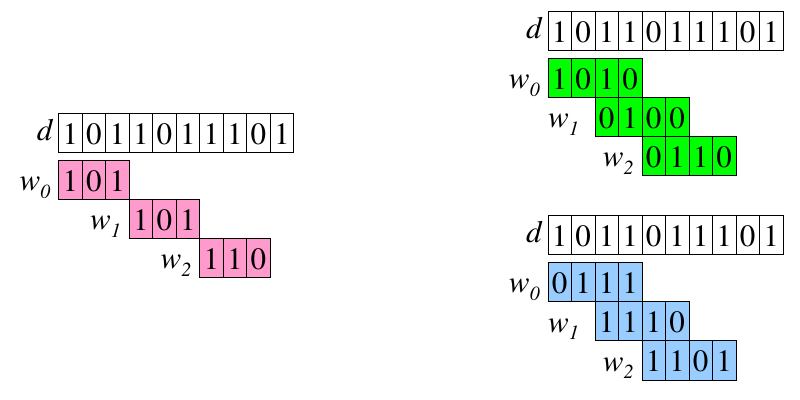
\includegraphics[scale=0.30]{images/Over.png}
				\caption{Overlapping window methods illustration}
				\end{center}
			\end{figure}

Let's assume that a $2^5$-ary method with an overlapp of $2$ bits: the window is each time shifted of $3$ 
bits instead of $5$. 
During the first exponentiation, the three first bits will be read and stored normally in the window but the two last bits will be two random ones,
and then the exponentiation of this window would take place.
At the next round of the exponentiation, this random will be compensate, and so on.

	
	  \item	\begin{tabularx}{\linewidth}{ p{16cm} p{1.5cm}}
			Clavier's square always method -\textit{Clavier 2011}-  & $0\%$ \\ 
			\end{tabularx}	
			\noindent
			Revisiting the Babylonians method replacing multiplications by squarings, thanks to 
			an old identity :
			\begin{center}			
				$x \times y = (\frac{x+y}{2})^2-(\frac{x-y}{2})^2$
			\end{center}
			It also has the advantage to be easily parallizable
			and it is always faster than Montgomery ladder technique. 
			In practice only atomic version of this technique should be used,
			can be optimized with a the sliding window method.
			\\

			\vspace{5mm}
			\textit{VS side channel cryptanalysis}\\
			immune against SvsM discrimination
			\vspace{5mm}
\end{itemize}





\subsubsection{Counter measures to fault injection}

\begin{itemize}
\item \begin{tabularx}{\linewidth}{ p{16cm} p{1.5cm}}
			Shamir's trick -\textit{1999}-  & $0\%$ \\ 
	  \end{tabularx}
	  \noindent A probabilistic test - \textit{e.g.} not always working - detecting if the 
	  forging has been faulted, the probability of detection increase with the length of $r$.
	  
		\begin{algorithm}[h]
			\KwIn{m, d, r, $r_p$ , $r_q$ , n}
			\KwOut{  $ y   =  x^d \mod n$, if genuine }
			 $ S_{r \times p}  =  m^e \mod r \times p$ \;
			 $ S_{r \times q}  =  m^e \mod r \times q$ 
			\If{ $S_{r \times p} \neq S_{r \times q \mod r}$ }
			{
			abort				
			}									 
			\Return{$ S = CRT(S_{r \times p}, S_{r \times q} ) $}\;
			\caption{Shamir's trick \textit{'Extend and reduce modulus'} }
		\end{algorithm}
		
		Remarks	
		\begin{itemize}
			\item Require the knowledge of $d$  -and not $d_p$, $d_q$-
			\item Does not detect fault during the recombination stage
			\item significantly longer exponentiation
		\end{itemize}	

\item \begin{tabularx}{\linewidth}{ p{16cm} p{1.5cm}}
			A faster countermeasure -\textit{1999}-  & $0\%$ \\ 
	  \end{tabularx}
	  \noindent A probabilistic test - \textit{e.g.} not always working - detecting if the 
	  forging has been faulted, the probability of detection increase with the length of $r$.
	  
		\begin{algorithm}[h]
			\KwIn{m, d, r, $r_p$ , $r_q$ , n}
			\KwOut{  $ y   =  x^d \mod n$, if genuine }	
			 $ S^{'} = CRT(S_{r \times p}, S_{r \times q} ) $ \;
			 $r=rnd$(32bits) \;
			 $S =S^{'} \mod n$\;
			 $S_j =S^{'} \mod j$\;			 
			 $ S_{p_r}  =  m^{d_p \mod r-1} \times j$ \;
			 $ S_{q_r}  =  m^{d_q \mod r-1} \times j$ \;
			 $ {S_j}^{'} =  CRT(S_{p_r}, S_{q_r} ) $  \;
			\If{ $ {S}^{'}  \neq {S_j}^{'}  \mod n$ }
			{
			abort				
			}									 
			\Return{$ S \mod r  $}\;
			\caption{A faster countermeasure}
		\end{algorithm}
		
		Remarks	
		\begin{itemize}
			\item Require the knowledge of $d$  -and not $d_p$, $d_q$-
			\item Does not detect fault during the recombination stage
		\end{itemize}
\newpage
\item \begin{tabularx}{\linewidth}{ p{16cm} p{1.5cm}}
			Joye \& Ciet's trick' -\textit{2002}-  & $0\%$ \\ 
	  \end{tabularx}
	  \noindent A probabilistic test - \textit{e.g.} not always working - detecting if the 
	  forging has been faulted, the probability of detection increase with the length of $r$.
	  
		\begin{algorithm}[h!]
			\KwIn{m, d, r, $r_p$ , $r_q$ , n}
			\KwOut{ $ y   =  x^d \mod n$ if genuine }	
			 $ S^{'} = CRT(S_{r \times p}, S_{r \times q} ) $ \;
			 $r_1=rnd$(32bits),  $r_2=rnd$(32bits)  \;
			 $S =S^{'} \mod n$\;
			 $S_j =S^{'} \mod j$\;			 
 $ S_{p}^{\star}  =  m^{d_p} \mod  p \times r_1,  S_{p}^{'}  =  m^{d_p \mod \phi(r_1)} \mod  r_1  $ \; 
 $ S_{q}^{\star}  =  m^{d_q} \mod  q \times r_2,  S_{p}^{'}  =  m^{d_p \mod \phi(r_2)} \mod  r_2  $ \;
			\If{ $S_{p}^{\star} \neq S_{p}^{'} \mod r_1$ or $S_{q}^{\star} \neq S_{q}^{'}  \mod r_2$}
			{
			abort				
			}									 
			\Return{$ S \mod r  $}\;
			\caption{A faster countermeasure}
		\end{algorithm}
		
		Remarks	
		\begin{itemize}
			\item Does not require the knowledge of $d$  -and not $d_p$, $d_q$-
			\item Detect fault during the recombination stage
		\end{itemize}

\item	\begin{tabularx}{\linewidth}{ p{16cm} p{1.5cm}}
			Masked Montgomery ladder technique -\textit{Fumaroli 2006}-  & $0\%$ \\ 
		\end{tabularx}	
			Exactly the same algorithm than the previous one but with a random value added.
			Exist also in a side channel analysis and fault attack resistant version: a checksum
			is initiated, recalculated at the end of each loop and removed at the end of the algorithm.	
\end{itemize}

%
%to do:
%fumarolli
%vigilant CRT
%Joye's BOS algo -broken-


	    	\chapter{About template attacks}	
	    		\begin{center}
	Original paper, presenting Template Attacks on stream cyphers with Point Of Interest \\
	\lokiquote{ches-2002-chari} 
\end{center}
\section{The original template attack}


Template attacks\footnote{
\lokiquote{wisa-2008-medwed},\lokiquote{wisa-2008-schmidt},\lokiquote{wisa-2008-herbst}
} 
have been introduced by \citeauthor*{ches-2002-chari}, from IBM research, in 2002, originally to attack stream-cypher and block-cypher cryptosystems and being able to break a system with very few recorded traces, possibly one.


Belonging to the family of side-channel attacks as it exploits the fact that power consumption
of depend on the data processed, it is however very different
from SPA/DPA and their variants of all order as template attack is a 
\textit{two steps attack}.

%\mathcal{H}

\subsection*{First step, the setup phase:}

A template attack begins exactly as DPA attacks does by selecting a target:
a variable that appears \textit{or not} during the computation and that will be written as
$h=h(m,k)$ a function of the plain-text and the key.
Another parallel with standards DPA attacks, is that exhaustive enumeration of the values
taken by this targeted variable will have to be practical in this attack.

For each of these possible values, many traces shall be recorded -around 1000- so that 
a 'template' could be built, characterizing with precision the noise of this packet by 
a multivariate normal distribution the noise that can be observed. 
This elaborated mathematical model, permit to approach a more complex leakage 
model than the linear one, as DPA/CPA is usually doing.

Note that in this description already lies several attacks in the 
definition of $h$, all with different feasibilities, we can cite the all inputs of an S-boxes, 
only the keys related to this S-box,
or the output of an S-box, or its hamming weight, etc... Depending on this definition
there will have more or less templates to built and then evaluate: and without surprise
the more templates there is the more powerful the attack is but also the 
less practicable the attack becomes...

To initiate the setup phase the definition of $h$ have to be chosen.
Then recorded traces will be sorted depending on the particular value $\hat{h}$  that  $h$ has for each of them.
Note that to characterise efficiently the distribution of the noise associated to one of the packet thereby defined each packet shall have its elements the most 'randomly chosen'
\footnote{a clearer definition of this meaningless expression is possible}.

\newpage
The template associated to the particular value $\hat{h}$ of the variable $h$, 
is the pair $ \mathcal{T}_{\hat{h}} = ( m_{\hat{h}} ,\Sigma_{\hat{h}} )$, where:
	\begin{itemize}
		\item $ m_{\hat{h}} $ is the average of the $\hat{h}$-packet 
		\item $ \Sigma_{\hat{h}} $ is built upon the noise covariance matrices of the $\hat{h}$-packet.
	\end{itemize}

Wikipedia - \textit{Covariance matrix} :\\
let's $\vec{X}$ be a vector composed of $n$ random variables 
$(X_i)_{1 \leq i \leq n}$,
each of them having a finite variance, then the covariance matrix 
$\Sigma_{ \vec{X} }$ is a 
$ n \times n $ matrix and is defined by
is defined by its components:
\begin{center}
	on the diagonal $\Sigma_{ \vec{X} }  = var(\vec{X})$ \\
	\vspace{1mm}
	out of the diagonal $\Sigma_{ \vec{X} }(i,j) = Cov(X_i, X_j)$
	\end{center} 
Where : 
\begin{center}
$Cov(X_i,X_j) = \mathbb{E}[(X_i-\mathbb{E}[X_i])(X_j-\mathbb{E}[X_j])]$
\end{center} 

\textbf{THEN:}
Keeping the same notations, to compute the covariance matrix 
$ \Sigma_{\hat{h}} $, requires to define :
\begin{center}
$X_1 = \{$  first points  of all traces $\}$ \\ 
$X_2 = \{$  second points of all traces $\}$ ...\\
defining $X$ as a vector with $poi$ elements 
\end{center}
The  matrix $ \Sigma_{\hat{h}} $ shall be a $poi \times poi$ 
matrix, because of size of $t-m_h$ ($poi$) in the following formulas.


\subsection*{Second step, the attack phase:}

At this point, after the setup phase, what we manage to built a formula to evaluate the conditional probability 
$ \mathscr{P}( \mathrm{A} | \mathrm{B} )$ of an event $\mathrm{A}$,'a trace is recorded' , happening if $\mathrm{B}$,
'$\mathcal{H}=h$', is certain. \\
A trace $t$ is recorded:
\begin{center}
$\mbox{\Huge}{ \mathscr{P}(t | h) = \frac{ 1 }{ \sqrt{ (2\pi)^p |{\Sigma_h}| } } 
				\exp^{( -\frac{1}{2} (t-m_h)^t {{\Sigma_h}}^{-1} (t-m_h) )}	
				}  $			
\end{center}
A noise $x$ is recorded:
\begin{center}
$\mbox{\Huge}{	\mathscr{P}(x_h | h)   =\frac{ 1 }{ \sqrt{ (2\pi)^p |{\Sigma_h}| } } 
				\exp^{( -\frac{1}{2} {x_h}^t {{\Sigma_h}}^{-1} x_h )}			
				}  $			
\end{center}
Where:
\begin{itemize}
	\item $ |{\Sigma_h}| $ is the determinant of the $ {\Sigma_h} $ matrix
	\item $ {{\Sigma_h}}^{-1} $ is the inverse of the $ {\Sigma_h} $ matrix
\end{itemize}


The Maximum likelihood principle:

When the attacker have a trace $t$ he/she then evaluate the probability
$\mathscr{P}(t | h)$ all the possible value of $h$. The output is constituted 
of all the value $k$, linked to $h$ such that the corresponding probability 
are sorted form the most probable to the less one.


The main interest of this attack is that the two steps can be done on two different,
but identical, chips. The setup phase can then be achieved on a clone of the targeted 
device, and in a second time only the attack phase is performed on the targeted device,
with very few power consumption records.

\underline{Proposition:}\\
Under the Gaussian assumption and if only recorded trace, noted $t$, is available, the maximum likelihood principle
while applied to two equally possible hypothesis simplifies to the following comparison:

$$\mbox{\Huge}{
				(t-m_{h0})^t {{\Sigma_{h0}}}^{-1} (t-m_{h0}) 
			   -(t-m_{h1})^t {{\Sigma_{h1}}}^{-1} (t-m_{h1})  \leq
			   \ln (|\Sigma_{h0}|)-ln(|\Sigma_{h1}|)	
				}  $$	
				where a decision is made in favor of $H_1$ if the above inequality is true and in favor of $H_0$ otherwise.
\newpage
\section{Practical improvements}
The previous attack is very powerful indeed due to the elaborated mathematical model underlying
but also absolutely impracticable in the real world, even with good computers for the same reason.
Hereafter are listed the two way of making Template Attack more feasible and finally a
   remark on the importance of signal processing before building the templates.
\begin{itemize}
	\item Point Of Interests: '\textit{reduced traces to some specific points}'\\
	The idea is to perform the attack not on the whole traces but 
	only on traces reduced to few decades of interesting points. 
	For each value of the selected variable has been recorded a packet of $n_i$ 
	traces,	of average $\mu_i(t)$ and of variance $\sigma_i(t)$, then different 
	functions of time can be considered to define Points of interest with the 
	abscissas of their highest pikes, sorted in term of efficiency:	 
	\begin{itemize}
		\item Chari\textit{\&al.} in \lokiquote{ches-2002-chari}  
		difference of average signals: 
		First proposed method for selection of points for some $i$ and $j$ select only 
		the points where large difference shows up.
		\begin{center}
		$d(t) =   \mu_i(t)-\mu_j(t)  $ 
		\end{center}
		
		\item Rechberger\textit{\&al.} in \lokiquote{wisa-2004-rechberger} 
		Sum Of Difference  of average signals:	
		Filter some noise but positive and negative quantity compensate each other and hide informations.		
		They also showed the crucial importance of two parameters to choose point of interest: 
		a minimum distance of one clock cycle and a heigh greater than the noise floor.
		\begin{center}
		$sod(t) =  \sum \limits_{ i < j }  ( \mu_i(t)-\mu_j(t) )	 $
		\end{center}
	
		\item Gierlichs\textit{\&al.} in \lokiquote{ches-2006-gierlichs}:
		 Sum Of Squared Difference of average signals:\\
		solve the previous problem but the noise is more present also, small contribution are crushed.
		\begin{center}
		$sosd(t) =  \sum \limits_{ i < j }   ( \mu_i(t)-\mu_j(t) )^2	 $
		\end{center}
		
		\item Agrawal\textit{\&al.} in 	\lokiquote{ches-2003-agrawal}: 
		Sum of squared $t$-values:\\
		This method seems to be the chosen one in most of the cases nowadays. 
		\begin{center}
		$sost(t) =  \sum \limits_{ i < j } 
		\frac{
 		 ( \mu_i(t)-\mu_j(t) )^2	}{
 		 (  \frac{ {\sigma_i}^2 }{n_i} + \frac{ {\sigma_j}^2 }{n_j} )(t) } $
		\end{center}
		where $n_i$ and $n_j$ are size of the different packet.
	\end{itemize}

	\item Principal Component Analysis: 
	'\textit{analyse only most importnant part of $\Sigma_h$}'\\
	Archambau \textit{\&al.} in \lokiquote{ches-2006-archambeau}
	published an article to apply the famous statistical method called 
	Principal component analysis which technique reduces the dimension of the 
	covariance matrix by projection into the subspace spanned by the eigenspaces
	of the highest eigenvalues.


	\item Signal processing and acquisition: 
	\textit{'analyse transformed traces'}
	\begin{itemize}
		\item  Rechberger\textit{\&al.} in \lokiquote{wisa-2004-rechberger} 
		In a practical study advised to perform template attacks not on the time 
		domain but on the frequency domain with significant improvement of the 
		result, especially for noisy traces.	
	
		\item  El Aabid\textit{\&al.} in 
		\lokiquote{jce-2012-elaabid} In a practical study showed 
		the crucial importance of two parameters: the chronological synchronization
		and the vertical scale. They shall be the same for all traces.	
	\end{itemize}

	\item Reduced matrix:
	\textit{'definition of the matrix $\Sigma_h$ can be simplified'}
	\begin{itemize}
		\item[1-]  Fill only the diagonal, computation of $\Sigma_h^{-1}$ trivial	
		\item[2-]  Stochastic attack, see section \ref{The_stochastic_attack}.		
	\end{itemize}
\end{itemize}

Normally nowadays every template attacks shall take in account those approaches.






\newpage
\section{Template based DPA attacks:}

Two ways to turn template attacks to more DPA like attack, \textit{i.e.} 
to attack recovering bits of the keys from 'a lot' of traces. The first 
one is applying template attacks to several available traces the second 
one is skipping the setup phase and give a new metric for DPA.

\subsection{Template attack with several traces}
 Bayes' theorem allows us to evaluate the probability of the event
 "the sub key used was $ k $ given that $ x $ is recorded". 
\begin{center}
$$\mbox{\huge}
{ \mathscr{P}(\mathcal{H}=\hat{h}| t) = 
\frac{ \mathscr{P}(t | \hat{h} )\mathscr{P}(\hat{h}) }{ \sum_j \mathscr{P}(t | h_j).\mathscr{P}(h_j) } }  $$
\end{center}
It also permit us to consider the case of a set of traces $\mathbf{T}$ available during the attack phase:
\begin{center}
$$\mbox{\Huge}{ 
\mathscr{P}(\mathcal{H}=\hat{h} | \mathbf{T}) =
\frac{
\left( \prod\limits_{i=1}^D\mathscr{P}(t_i | \hat{h}) \right).\mathscr{P}(\hat{h})
}{
\sum\limits_{l=1}^H
\left( \left( \prod\limits_{i=1}^D\mathscr{P}(t_i | h_l) \right).\mathscr{P}(h_l)\right)
}
				}  $$			
\end{center}


\subsection{DPA-Template attack}
The classical DPA-decision metric can be improved thanks the notion of template even is no 
template is actually build using the inequality mentioned previously.

Let $H_i$ be one of the considered hypothesis by a DPA attack, and $H_v$ the value of the selection function.
To those two equally possible hypothesis can be applied the inequality presented earlier. Then the obtained metric is not evaluable because two parameters are not known problem solved by giving an estimation of those two.

This attack is among the most powerful side channel attack, because it can efficiently adapted to makes algorithms,
this is this attack, in its naive version, that Inspector implemented note however that the selection of the point 
of interests is critical.


\section{Template attacks on symmetrical algorithms}
\subsection*{What has been published}
\begin{itemize}  
	\item[-] In 2003, Chari\textit{\&al.} in 
\lokiquote{ches-2002-chari}
gave the first description of a two steps side channel attacks, with elaborated model for noise.

	\item[-] In 2003, Agrawal\textit{\&al.} in 
\lokiquote{ches-2002-agrawal} 
improved significantly the template attack combining multiple side channel 
such as power and EM simultaneously.
They also improved the DPA attack defining a new metric by using the Gaussian assumption, turning 
	 the DPA attack to a two steps attacks and if the setup  phase was impossible to perform
	they give a way to approximates this one. Quoting Elisabeth Oswald 'Template based DPA attack 
	constitute the strongest the strongest kind of DPA attack.
			  
	\item[-] In 2005, Agrawal\textit{\&al.} in 
\lokiquote{ches-2005-agrawal}
defined the 'single bit template attack' where the targeted variable is a single bit
and the 'template enhanced DPA attack' mixing template and DPA attack (Warning)	 
They also break a masked DES and AES basically building template with a chip with a biased RNG 
and then exploiting those on the same chip with a perfect RNG.


	\item[-] In 2006, Mangard\textit{\&al.} in 
	\lokiquote{ctrsa-2007-oswald} 
the authors claim that 'in the scenario of template attacks, masking does not improve the security of an implementation... '
They used template based DPA attacks to attack masked version of the DES and AES, 
reference to the masks in \lokiquote{ches-2001-akkar} and 
\lokiquote{sacrypt-2004-bloomer},
with devastating conclusions, if an biased PRNG is available during the setup phase!
The attack phase just this line is changing.
\begin{center}$$\mbox{\huge}{ \mathscr{P}(t | h_j ) = 
{ \sum_j \mathscr{P}(t | h_j \wedge m).\mathscr{P}(m) } }  $$
\end{center} 

In this same paper, combination of HODPA and template attack is also studied: to
unleash the maximum of correlation in a 2$^{nd}$ order attack or to force a bias 
in the collected traces. 

	\item[-] In 2007, El Aabid\textit{\&al.} in 
	\lokiquote{eprint-2007-aabid} 
	claimed that the real target of template attack was the key schedule. 
Instead of the naive definition of $h$ sorting the traces depending on value of the sub-key used,
he improved the sorting using the following functions:\\\
$h= k $\\
$h= k \oplus LS(k)  $\\
$h= k \oplus LS^2(k)  $\\
where $LS$	is the left shift function used in the key schedule of the DES algorithm. 
In this article  they recognize that the first function is suitable for a 'blind' attacker

\item[-] \lokiquote{phdthesis-ElAabid-2012}.
\end{itemize}

\subsection*{Definitions for $h$}
Here only the case of the DES algorithm is considered and 
$Input$ and $Output$ will represent the respective input and output of some S-box.

			\begin{tabularx}{\linewidth}{ p{4cm}  p{4cm}  p{4cm}}
			$ h  = Input$						& $2^{12}$ templates to build& \\
			$ h  = k $ 							& $2^{6}$ templates to build& \\
			$ h  = k \oplus LS(k)  $ 			& $2^{6}$ templates to build& \\
			$ h  = k \oplus LS^2(k)  $ 			& $2^{6}$ templates to build& \\
			$ h  = Output $						& $2^{4}$ templates to build& \\
			$ h  = \omega_\mathcal{H}(Input) $ 	& $5$ templates to build& 
			\end{tabularx}	
			
			
\subsection*{Matrix}

\begin{center}
\begin{savenotes}
\begin{tabular}{p{.5cm}p{.5cm}p{.5cm}p{.5cm}p{4.5cm}}
           \rotatebox{70}{ Naked DES } 
         & \rotatebox{70}{ Splited DES }
    	 & \rotatebox{70}{ Masked DES 
				\footnote{The transforming masked method
				\lokiquote{ches-2001-akkar}
				 (one mask)}	} 
    	 & \rotatebox{70}{ Masked DES 
    	 		\footnote{The transforming masked method
		    	 \lokiquote{ches-2001-akkar} 
		    	 (two masks)} }    	 			
    	 & References\\    	 
\end{tabular}\\
\begin{tabular}{|p{.5cm}|p{.5cm}|p{.5cm}|p{.5cm}|p{4.5cm}|}   	
	\hline  $\bullet$ & & & & \cite{ches-2002-chari}\\
	\hline  $\bullet$ & & & & \cite{ches-2002-agrawal} \\
	\hline  $\bullet$ & & $\circ$ & & \cite{wisa-2004-rechberger} \\
	\hline  $\bullet$ & & $\bullet$ & ? & \cite{ches-2005-agrawal}\\
	\hline  $\bullet$ & & & & \cite{eprint-2007-aabid}\\				
	\hline 
\end{tabular}\\
\end{savenotes}
\end{center}



\newpage
\section{Template attacks on asymmetrical algorithms}

In this section we only consider the two most used asymmetrical algorithms, 
namely RSA and ECC, because of their common point that is they share a family of algorithms 
to perform the central operation on which mainly depends their security. 

This is modular exponentiation for RSA and scalar multiplication for ECC, both 
taking place in some finite fields. In RSA the the first 
of those algorithms is the well known square-and-multiply algorithm to which is 
corresponding the double-and-add algorithm for elliptic curves.

\subsection*{What has been published}

\begin{itemize}  
	\item[-] In \lokiquote{wisa-2008-medwed} is
	showed the feasibility of template attacks on asymmetrical algorithm:
	on a unmasked ECDSA implemented with the double-and-add-always algorithm
	and also with the sliding window version of this algorithm. They gave also conditions
	so their attack to work with scalar blinding \footnote{corresponding to exponent blinding in RSA}
	and for Point Blinding \footnote{corresponding to message blinding in RSA}.
	A counter measure is to randomize the base point \footnote{corresponding to nothing in RSA}.
	
	\item[-] In \lokiquote{wisa-2008-herbst} is
	showed the feasibility of template attacks on masked asymmetrical algorithm:
	on a RSA implemented with a masked version of the Montgomery ladder exponentiation.
		
	
	\item[-] In \lokiquote{sacrypt-2008-amiel} is
	showed a theoretical presentation of template attacks on atomic versions of 
	the double-and-add algorithm and of the square-and-multiply algorithm.
	In this article is said that a device with a high level of side channel 
	leakage, even with a masked exponent, could be vulnerable to their attack.
	
		
	\item[-] In \lokiquote{ijis-2011-hanley} is
	showed an extension of the previous article giving a practical presentation 
	of template attacks	on \textit{atomic} versions of the double-and-add algorithm 
	and of the square-and-multiply algorithm.
	Plus, the attack described in this paper do not require any open device to built
	its template. 	
	
	\item[-] \lokiquote{acns-2011-schindler}
	revisit the paper of P.A Fouque "Power attack on small RSA public exponent" 
	which can if some bits exponent are known the recover the all exponent, 
	to make it more error tolerant and then more practical. Case of Square and always Multiply
	or for Double and always Add.
\end{itemize}

\section{The stochastic attack}
\label{The_stochastic_attack}
Schindler\textit{\&al.} in \lokiquote{ches-2005-schindler} 
publish a variant of template attack: the Stochastic attack also known as the regression model.
This attack find the key answering to the following question:
'among all the linear leakage models that can be build with $N$ simulations of the targeted variable 
and the recorded trace, which in the end corresponds the best to the recorded trace ?'

First let's assume that  the deterministic part of the leakage is simply
$\delta(x) = \alpha_{-1}  + \sum \limits_{i=0}^{n} \alpha_i.x_i $ and that the target variable $h$ got $n$ bits, 
 and that $ \left( l_{\hat{h},i}\right)_{1 \leq i \leq N}$ is one measure set of $N$ measurements.
 				\begin{equation*}
				L = 
				\begin{bmatrix}
				l_{{h},1}\\
				\vdots\\
				l_{{h},N}\\
				\end{bmatrix}
				\end{equation*}
Now for every possible value $\hat{h}$ of $h$ let's assume that
$ \left( v_{\hat{h},i}\right)_{1 \leq i \leq N}$ are the $N$ corresponding hypothesis about the deterministic 
part of the leakage. And let's take a look at the contribution of each bits of $v$:
				\begin{equation*}
				M = 
				\begin{bmatrix}
				1 & v_{\hat{h},1}[0]  &\ldots & v_{\hat{h},1}[n-1] \\
				  & \vdots &          & \vdots \\
				1 & v_{\hat{h},N}[0]  &\ldots & v_{\hat{h},N}[n-1]
				\end{bmatrix}
				\end{equation*}
The leakage model given by the hypothesis '$h = \hat{h}$' is:
\begin{center}
$\alpha_{\hat{h}} = (\alpha_{\hat{h},{-1}}, \hdots , \alpha_{\hat{h},{n-1}}) = ( M^\top .M)^{-1} . (M^\top .L)$
\end{center}
And the signal of decision for this hypothesis is:
\begin{center}
$\Delta_{\hat{k}}  = \frac{|L-M.\alpha_{\hat{k}}|_2}{\sqrt{Var(L)}} $
\end{center}
Then the most probable value for $h$ is the one minimising  $\Delta_{\hat{k}}  $

Question: some claim that the stochastic method is just a normal template attack replacing
the covariance matrix for the identity matrix... ?

\newpage
\section{The power consumption model \& notations}

The classical presentation is the following one. It is assumed when considering 
a sensitive variable $V_h$ \footnote{This notation ... }
, the leakage, $L$ to be composed of two parts: 
a deterministic part, $\delta$ and the noise independent from $V_h$, \textit{i.e.} 
independent from the plain text and the key.
\begin{center}
	$L_h = \delta(V_h)  + B$
\end{center}
Then if $N$ measurements are done, the previous equation implies:
\begin{center}
	$\forall i \leq N, \hspace{5mm}  l_{h,i}= \delta(v_{h,i})  + b_i$
\end{center}
One of the more general \textit{symmetrical} model for approaching the function $\delta$ of a variable $x$ of $d$ is given by:
\begin{center}
				$\delta(x) = \alpha_{-1}  + \sum \limits_{i=0}^{n} \alpha_i.x_i 
			+ \sum \limits_{i_1 \neq i_2=0}^{n} \alpha_{i_1,i_2}.x_{i_1,i_2} + \hdots + 
			  \sum \limits_{i_1 \neq \hdots \neq i_d=0}^{n} \alpha_{i_1,\hdots,i_d}.x_{i_1,\hdots,i_d} $
\end{center} 
Hypothesis to simplify this model:
\begin{itemize}
	\item[-LID:]Leakage Interpolation Degree:\\
	A good approximation of $\delta$ can be obtained with a polynomial of smaller multivariate degree, $n <  d$.
	\item[-IBL:]Independent Bit Leakage:\\
	A good approximation of $\delta$ can be obtained with a linear function, $n=1$.
	\item[-EHQ:]Equivalent Homogeneous Contribution:\\
	A good approximation of $\delta$ can be obtained assuming that 
	each homogeneous polynomial constituting $\delta$ have independently the same coefficient.
\end{itemize}
Questions :\\
DPA/CPA etc IBL ?, EHQ ?\\
Template attacks LID with n=2? EHQ ?\\




	\chapter{Latex definition \& tricks}
		\lokiquote{spec-2009-dss}
\lokiquote{spec-2002-mac}
\lokiquote{spec-2001-aes} 
\lokiquote{spec-2000-certicom}
\lokiquote{spec-2000-dss}
\lokiquote{spec-1977-des} 
\lokiquote{spec-1999-iso9797-1} 
\lokiquote{phd-Goyet-2012}
\lokiquote{phd-ElAabid-2012}
\lokiquote{phd-Verneuil-2012}
\lokiquote{phd-Medwed-2012}
\lokiquote{M2Thesis-Timmerman-2011}
\lokiquote{M2Thesis-Timmerman-2011}
\lokiquote{phd-Gierlichs-2011}
\lokiquote{M2Thesis-Papachristodoulou-2010}
\lokiquote{M2thesis-Hogenboom-2010}
\lokiquote{M2Thesis-Kruti-2010}
\lokiquote{M2Thesis-Timmerman-2011}
\lokiquote{phd-Berzati-2009}
\lokiquote{phd-Wiseur-2010}
\lokiquote{phd-Waldir-2008}
\lokiquote{phd-Clavier-2007}
\lokiquote{phd-DeCanniere-2007}
\lokiquote{phd-Guilley-2007}
\lokiquote{phd-Giraud-2007}
\lokiquote{phd-LemkeRust-2007}
\lokiquote{phd-Longa-2007}
\lokiquote{phd-Piret-2005}
\lokiquote{M2Thesis-Muir-2004}
\lokiquote{phd-Bevan-2004}
\lokiquote{phd-Medwed-2003}
\lokiquote{M2Thesis-Hasselstrom-2003}
\lokiquote{phd-Oswald-2003}
\lokiquote{M2Thesis-Schramm-2003}
\lokiquote{phd-Batina-2002}
\lokiquote{phd-Messerges-2000}
\lokiquote{phd-Dehem-2000}
\lokiquote{ppt-Chu-ComplexeSurfaces}
\lokiquote{ppt-Chu-ComplexeSurfaces}
\lokiquote{ppt-Joye-EllipticCurveCryptography}
\lokiquote{book-2012-sedgewick}
\lokiquote{book-2012-joye}
\lokiquote{book-2011-encrypt}
\lokiquote{book-2008-tahe}
\lokiquote{book-2007-neubauer}
\lokiquote{book-2006-oswald}
\lokiquote{book-2004-stern}
\lokiquote{book-2004-goldreich}
\lokiquote{book-2004-hankerson}
\lokiquote{book-2002-joliffe}
\lokiquote{book-2001-goldreich}
\lokiquote{book-2000-rankl}
\lokiquote{book-2000-schneier}
\lokiquote{book-2000-silverman}
\lokiquote{book-1994-wart}
\lokiquote{book-1996-menezes}
\lokiquote{book-1991-koblitz}
\lokiquote{ches-2015-tuto-mukhopadhyay}
\lokiquote{ches-2015}
\lokiquote{ches-2012-murdoch-ppt}
\lokiquote{corr-2012-bond}
\lokiquote{ches-2012-heyse}
\lokiquote{ches-2012-ruhrmair}  
\lokiquote{ches-2012-fei} 
\lokiquote{ches-2012-reparaz} 
\lokiquote{ches-2012-schloumlsser}
\lokiquote{ches-2012-kerckhof}      
\lokiquote{ches-2012-lee} 
\lokiquote{ches-2012-gottert}   
\lokiquote{ches-2012-debraize}  
\lokiquote{ches-2012-debraize}      
\lokiquote{ches-2012-cheng}     
\lokiquote{ches-2012-sarkar}  
\lokiquote{ches-2012-bernstein}      
\lokiquote{ches-2012-czypek}      
\lokiquote{ches-2012-faust}     
\lokiquote{ches-2012-bilgin}      
\lokiquote{ches-2012-guneysu}     
\lokiquote{ches-2012-knezevic}      
\lokiquote{ches-2012-debraize}      
\lokiquote{ches-2012-fouque}      
\lokiquote{ches-2012-briais}  
\lokiquote{ches-2012-moradi}  
\lokiquote{ches-2012-moss} 
\lokiquote{ches-2012-vanderleest}
\lokiquote{ches-2012-vielhaber} 
\lokiquote{ches-2012-gerard}        
\lokiquote{ches-2012-maes}  
\lokiquote{ches-2012-subhadeep}       
\lokiquote{ches-2012-medwed}        
\lokiquote{ches-2012-vielhaber}       
\lokiquote{ches-2012-matsuda}       
\lokiquote{ches-2012-oren}  
\lokiquote{ches-2011-goubin}  
\lokiquote{ches-2011-kim} 
\lokiquote{ches-2011-clavier} 
\lokiquote{ches-2011-fan} 
\lokiquote{ches-2011}       
\lokiquote{ches-2010-tunstall}  
\lokiquote{ches-2010-prouff}  
\lokiquote{ches-2010-berzati} 
\lokiquote{ches-2010-longa} 
\lokiquote{ches-2010}
\lokiquote{ches-2009-batina}  
\lokiquote{ches-2009-renauld} 
\lokiquote{ches-2009-coron} 
\lokiquote{ches-2009-coron-2}
\lokiquote{ches-2009}       
\lokiquote{ches-2008-baddam}  
\lokiquote{ches-2008}
\lokiquote{ches-2007-bogdanov}  
\lokiquote{ches-2007}
\lokiquote{ches-2006-lee} 
\lokiquote{ches-2006-prouff}  
\lokiquote{ches-2006-stebila} 
\lokiquote{ches-2006-archambeau}
\lokiquote{ches-2006-brier} 
\lokiquote{ches-2006-fouque}  
\lokiquote{ches-2006-gierlichs}
\lokiquote{ches-2006}
\lokiquote{ches-2005-joye}
\lokiquote{ches-2005-agrawal} 
\lokiquote{ches-2005-canright}  
\lokiquote{ches-2005-peeters} 
\lokiquote{ches-2005-popp}  
\lokiquote{ches-2005-schindler} 
\lokiquote{ches-2005}
\lokiquote{ches-2004-hars}  
\lokiquote{ches-2004-brier}
\lokiquote{ches-2004-fouque}  
\lokiquote{ches-2004-ledig} 
\lokiquote{ches-2004-schramm} 
\lokiquote{ches-2004}
\lokiquote{ches-2003-agrawal}
\lokiquote{ches-2003-coron} 
\lokiquote{ches-2003-fouque}  
\lokiquote{ches-2003} 
\lokiquote{ches-2002-trichina}  
\lokiquote{ches-2002-agrawal}
\lokiquote{ches-2002-chari}
\lokiquote{ches-2002-itoh}  
\lokiquote{ches-2002-joye}  
\lokiquote{ches-2002}
\lokiquote{ches-2001-akkar}   
\lokiquote{ches-2001-clavier} 
\lokiquote{ches-2001-sakurai}
\lokiquote{ches-2001}      
\lokiquote{cciam-1997-clavier}  
\lokiquote{ches-2000-coron} 
\lokiquote{ches-2000}
\lokiquote{ches-1999-goubin}  
\lokiquote{ches-1999-messerges} 
\lokiquote{cosade-2012-darolt}  
\lokiquote{cosade-2012-hutter}  
\lokiquote{cosade-2011-wang}  
\lokiquote{cosade-2010-medwed}  
\lokiquote{cosade-2010-bar} 
\lokiquote{fse-2004-akkar}  
\lokiquote{fse-2003-akkar}  
\lokiquote{fse-1994-wheeler}  
\lokiquote{crypto-2009-coron} 
\lokiquote{crypto-2004-okeya} 
\lokiquote{crypto-2003-patarin} 
\lokiquote{crypto-2000-biehl} 
\lokiquote{crypto-1999-coron} 
\lokiquote{crypto-1999-kocher}
\lokiquote{crypto-1998-koblitz} 
\lokiquote{crypto-1996-kocher}  
\lokiquote{crypto-1986-barrett} 
\lokiquote{crypto-1985-kochanski} 
\lokiquote{eurocrypt-2013-prouff} 
\lokiquote{eurocrypt-2013-bertonni} 
\lokiquote{eurocrypt-2009-standaert}  
\lokiquote{eurocrypt-2003-ciet} 
\lokiquote{eurocrypt-1997-boneh}
\lokiquote{eurocrypt-1992-brickell} 
\lokiquote{asiacrypt-2010-oswald} 
\lokiquote{asiacrypt-1998-boneh}  
\lokiquote{latincrypt-2012-gierlichs} 
\lokiquote{latincrypt-2011-aranha}
\lokiquote{latincrypt-2010-schmidt} 
\lokiquote{africacrypt-2009-joye} 
\lokiquote{indocrypt-2011-clavier}  
\lokiquote{indocrypt-2011-clavier-ppt}  
\lokiquote{indocrypt-2007-fumaroli} 
\lokiquote{ctrsa-2013-bauer}
\lokiquote{ctrsa-2012-maghrebi}
\lokiquote{ctrsa-2012-batina}
\lokiquote{ctrsa-2011-witteman}
\lokiquote{ctrsa-2011-brown}
\lokiquote{ctrsa-2011}
\lokiquote{ctrsa-2010}
\lokiquote{ctrsa-2009-berzati}  
\lokiquote{ctrsa-2009-berzati-ppt}  
\lokiquote{ctrsa-2009}
\lokiquote{ctrsa-2008}
\lokiquote{ctrsa-2007-oswald} 
\lokiquote{ctrsa-2007}       
\lokiquote{ctrsa-2006-schramm}  
\lokiquote{ctrsa-2006-oswald} 
\lokiquote{ctrsa-2006}
\lokiquote{ctrsa-2005}
\lokiquote{ctrsa-2004-fisher}                    
\lokiquote{ctrsa-2004}
\lokiquote{ctrsa-2003}
\lokiquote{ctrsa-2002}
\lokiquote{ctrsa-2001-brown}  
\lokiquote{ctrsa-2001}
\lokiquote{ctrsa-2010-gierlichs}  
\lokiquote{ctrsa-2010-coron}  
\lokiquote{crisis-2013-bouffard}  
\lokiquote{cardis-2004-guilley} 
\lokiquote{pkc-2006-muller} 
\lokiquote{pkc-2003-antipa} 
\lokiquote{pkc-2001-joye} 
\lokiquote{acns-2012-piret} 
\lokiquote{scn-2008-coron}  
\lokiquote{icassp-2007-le}  
\lokiquote{arith-2007-hasenplaugh}  
\lokiquote{fcds-2011-anderson}  
\lokiquote{sacrypt-2013-delerablee} 
\lokiquote{sacrypt-2011-moller} 
\lokiquote{sacrypt-2010-pan}  
\lokiquote{sacrypt-2009-joye}
\lokiquote{sacrypt-2008-amiel}
\lokiquote{sacrypt-2007-amiel}  
\lokiquote{sacrypt-2003-walter} 
\lokiquote{acrypto-1998-lopez}  
\lokiquote{icisc-2011-kramer} 
\lokiquote{icisc-1999-lim}  
\lokiquote{acisp-2009-tunstall} 
\lokiquote{fpl-2006-standaert}  
\lokiquote{fpl-2006-kamoun}
\lokiquote{host-2010-fan} 
\lokiquote{cute-2012-yeon}      
\lokiquote{iscsc-2009-maghrebi} 
\lokiquote{ecrypt-2007-aumonier}
\lokiquote{wisa-2009-hanley}  
\lokiquote{wisa-2008-herbst}  
\lokiquote{wisa-2008-medwed}      
\lokiquote{wisa-2008-schmidt}   
\lokiquote{wisa-2008-miret}
\lokiquote{wisa-2004-rechberger}        
\lokiquote{fdtc-2011-woudenberg}  
\lokiquote{fdtc-2008-schmidt}
\lokiquote{fdtc-2006-boreale}
\lokiquote{fdtc-2005-ciet}
\lokiquote{dft-2012-reggazoni}  
\lokiquote{tosca-2011-ruiter}
\lokiquote{usenix-1999-messerges}
\lokiquote{usenix-1999-messerges}
\lokiquote{usenix-1999-messerges}
\lokiquote{iccd-2001-ploog} 
\lokiquote{jofc-2011-batina}  
\lokiquote{eprint-2013-sidorenko}
\lokiquote{eprint-2013-rauzy}
\lokiquote{eprint-2012-krenn}
\lokiquote{eprint-2012-sarkar}
\lokiquote{eprint-2012-belenky}
\lokiquote{eprint-2012-hanley}
\lokiquote{eprint-2012-oren}
\lokiquote{eprint-2011-maghrebi}
\lokiquote{eprint-2011-hanley}
\lokiquote{eprint-2011-roy}
\lokiquote{eprint-2010-clavier}
\lokiquote{eprint-2009-dent}
\lokiquote{eprint-2008-wang}
\lokiquote{eprint-2007-aabid}
\lokiquote{eprint-2007-bard}  
\lokiquote{eprint-2007-lee}
\lokiquote{eprint-2005-avanzi}
\lokiquote{eprint-2005-avanzi}
\lokiquote{eprint-2006-courtois}
\lokiquote{eprint-2004-bernstein}
\lokiquote{eprint-2003-brier}
\lokiquote{eprint-2003-lemmermeyer}
\lokiquote{eprint-2003-ciet}
\lokiquote{eprint-2003-amhuller}
\lokiquote{eprint-2000-hijningen}
\lokiquote{ieeetc-2007-bogdanov}
\lokiquote{ieeetc-2005-montgomery}
\lokiquote{eprint-2003-brier}
\lokiquote{ieeetc-2000-joye}
\lokiquote{unigratz-2012-krenn} 
\lokiquote{unigratz-2012-krenn-ppt} 
\lokiquote{unigratz-2011-krenn-ppt} 
\lokiquote{unigratz-2011-krenn2-ppt}  
\lokiquote{unigratz-2009-heuberger-ppt} 
\lokiquote{unibordeau-2006-bergson} 
\lokiquote{unigratz-2012-krenn-ppt} 
\lokiquote{uniparma-2004-rizzo} 
\lokiquote{CanJMath-2008-blake}
\lokiquote{jce-2012-elaabid}
\lokiquote{jce-2012-moreno}
\lokiquote{cciam-1997-joye}
\lokiquote{stoc-2007-furer} 
\lokiquote{mlkdb-1997-mavroeidis} 
\lokiquote{ietifs-2011-mangard}     
\lokiquote{iolts-2006-kulikowski} 
\lokiquote{matcomp-2008-dimitrov} 
\lokiquote{matcomp-2008-dimitrov} 
\lokiquote{sbcci-2010-legal}  
\lokiquote{wircs-2010-abdi}
\lokiquote{jofnt-2012-heuberger}
\lokiquote{qjmam-2009-booth}
\lokiquote{issc-2008-tunstall}  
\lokiquote{esorics-2007-lemkerust}  
\lokiquote{cje-2012-liu}  
\lokiquote{corr-2012-bond}
\lokiquote{ijns-2002-lin} 
\lokiquote{psim-1995-Karatsuba} 
\lokiquote{aaecc-2011-poulakis} 
\lokiquote{gcc-2009-kreuzer}      
\lokiquote{asiacs-2008-Lee}       
\lokiquote{algo-2006-avanzi}  
\lokiquote{dimacs-1999-abrahams}  
\lokiquote{iisitt-2006-oluwatope} 
\lokiquote{ijis-2011-hanley}  
\lokiquote{preprint-2009-papachristodoulou}
\lokiquote{preprint-2008-dent}  
\lokiquote{preprint-2002-bernstein}
\lokiquote{preprint-2006-bernstein}  
\lokiquote{preprint-1994-koc} 
\lokiquote{birthday-2012-standaert}
\lokiquote{birthday-2012-joye}
\lokiquote{dcc-2001-avanzi} 
\lokiquote{dcc-2000-solinas}  
\lokiquote{sigmobile-2011-shannon}  
\lokiquote{eatcs-2003-fortnow}
\lokiquote{ieeemicro-1996-koc}
\lokiquote{microj-2013-cilio}		
		\newpage
From the natbib package
cite: %\sort{ches-2002-chari}{1}: cite an author with the link\\
nocite: \nocite{ches-2002-chari}: the paper is in the biblio, but no link papers in the text\\
citeauthor: \citeauthor{ches-2002-chari}: cite an author name\\
citeauthor*: \citeauthor*{ches-2002-chari}: cite all authors name\\
citet: \citet{ches-2002-chari}: cite an author with the link\\
citet*: \citet*{ches-2002-chari}: cite all author with the link\\
citep: \citep{ches-2002-chari}: cite an author with the link\\
citep*: \citep*{ches-2002-chari}: cite all author with the link\\
\lokiquote{ches-2002-chari}

		\bibliography{bibliographie}
		\printindex
\end{document}

%%%%%%%%%%%%%%%%%%%%%%%%%%%%%%%%%%%%%%%%%%%%%%%%%%%%%%%%%%%%%%%%%%%%%%%%%%%%%%%%%%%%%%%%%%%%%%%%
